\section{Физика элементарных частиц}
\begin{frame}{Физика частиц: содержание}
    \tableofcontents[currentsection, subsectionstyle=show/show/hide]
\end{frame}
\subsection{Частицы}
\begin{frame}
    \begin{figure}
        \begin{centering}
            \includegraphics[width=0.7\textwidth]{sm}
        \end{centering}
    \end{figure}
\end{frame}

\subsection{Ускорители}
\begin{frame}
    \begin{columns}
        \begin{column}{0.5\textwidth}
            \begin{figure}
                \begin{centering}
                    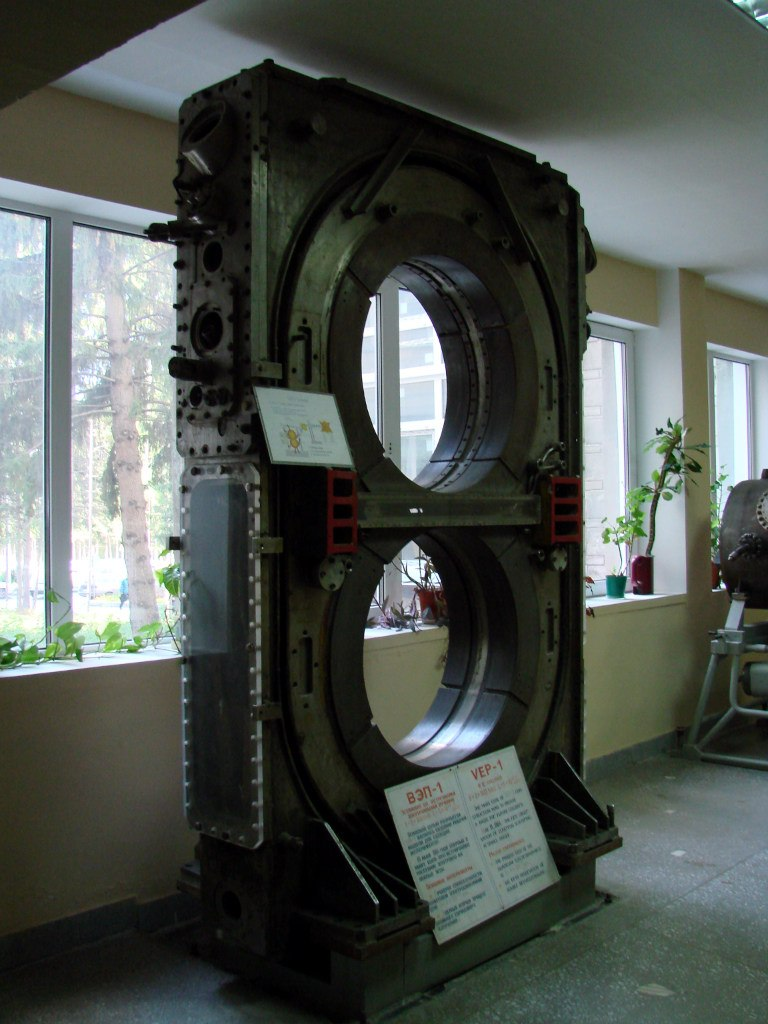
\includegraphics[width=0.7\textwidth]{vepp1}
                \end{centering}
            \end{figure}
        \end{column}
        \begin{column}{0.5\textwidth}
            \begin{figure}
                \begin{centering}
                    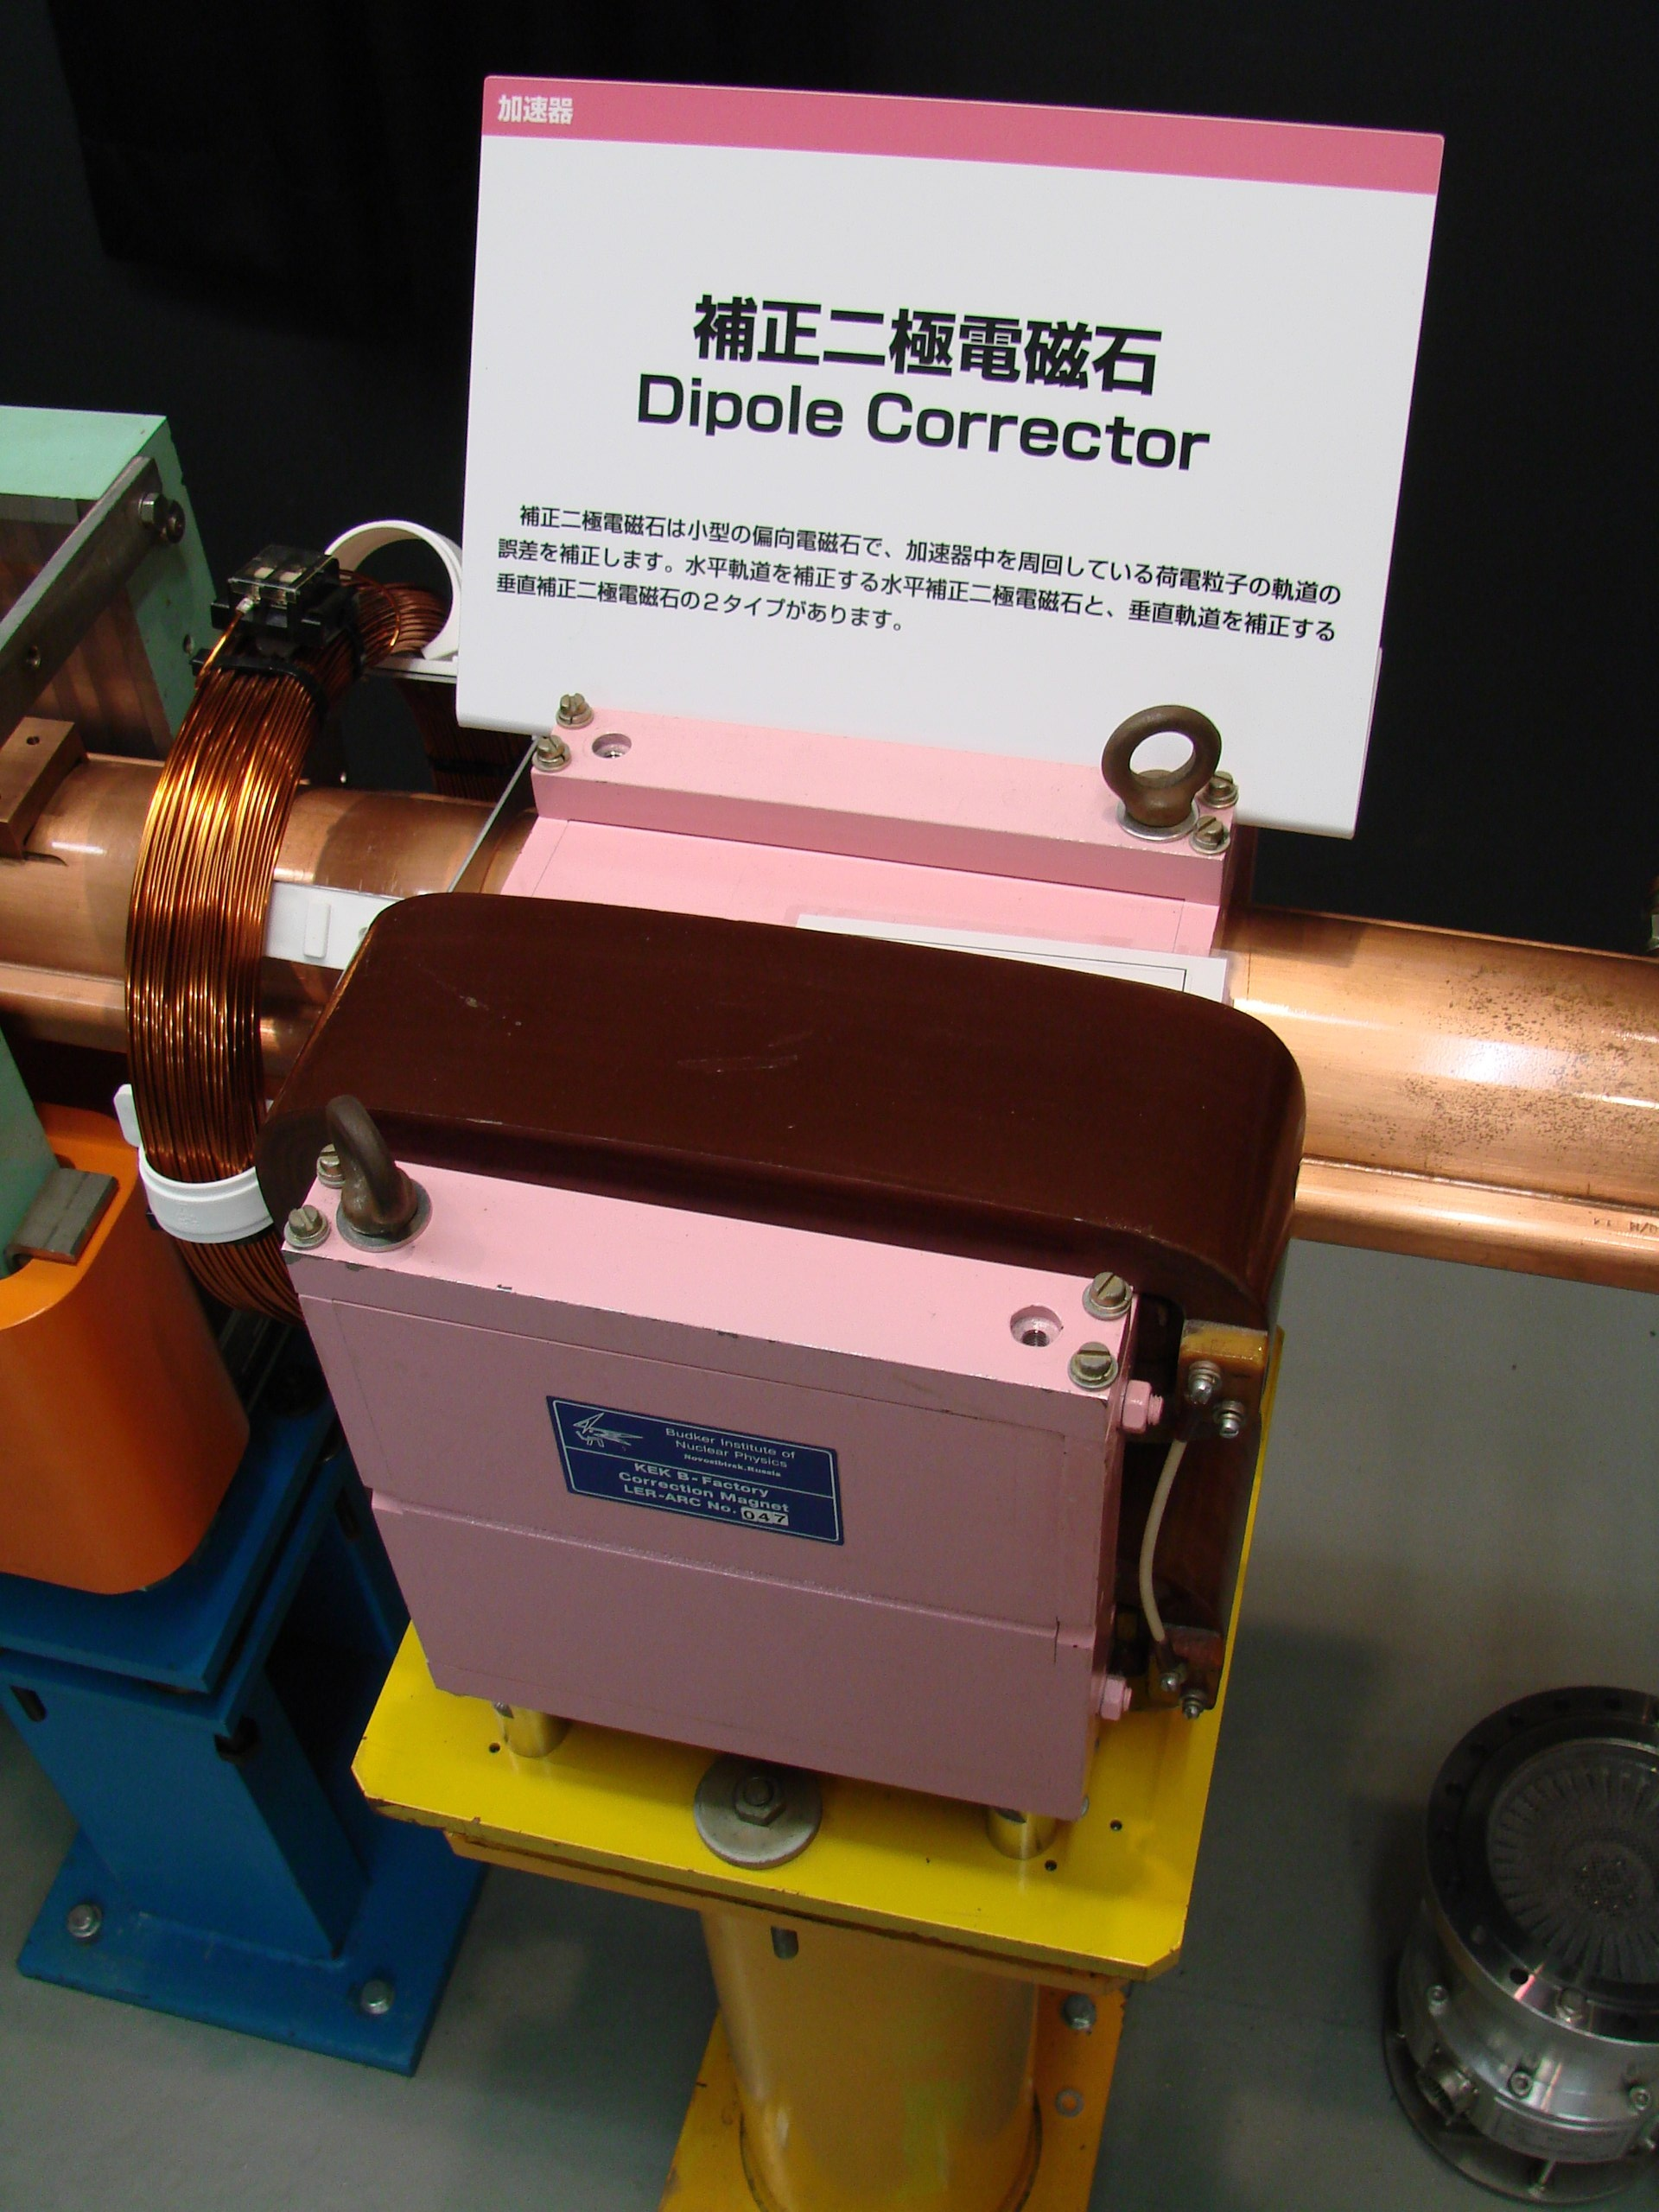
\includegraphics[width=0.7\textwidth]{dipole}
                \end{centering}
            \end{figure}
        \end{column}
    \end{columns}
\end{frame}


\begin{frame}
    \begin{figure}
        \begin{centering}
            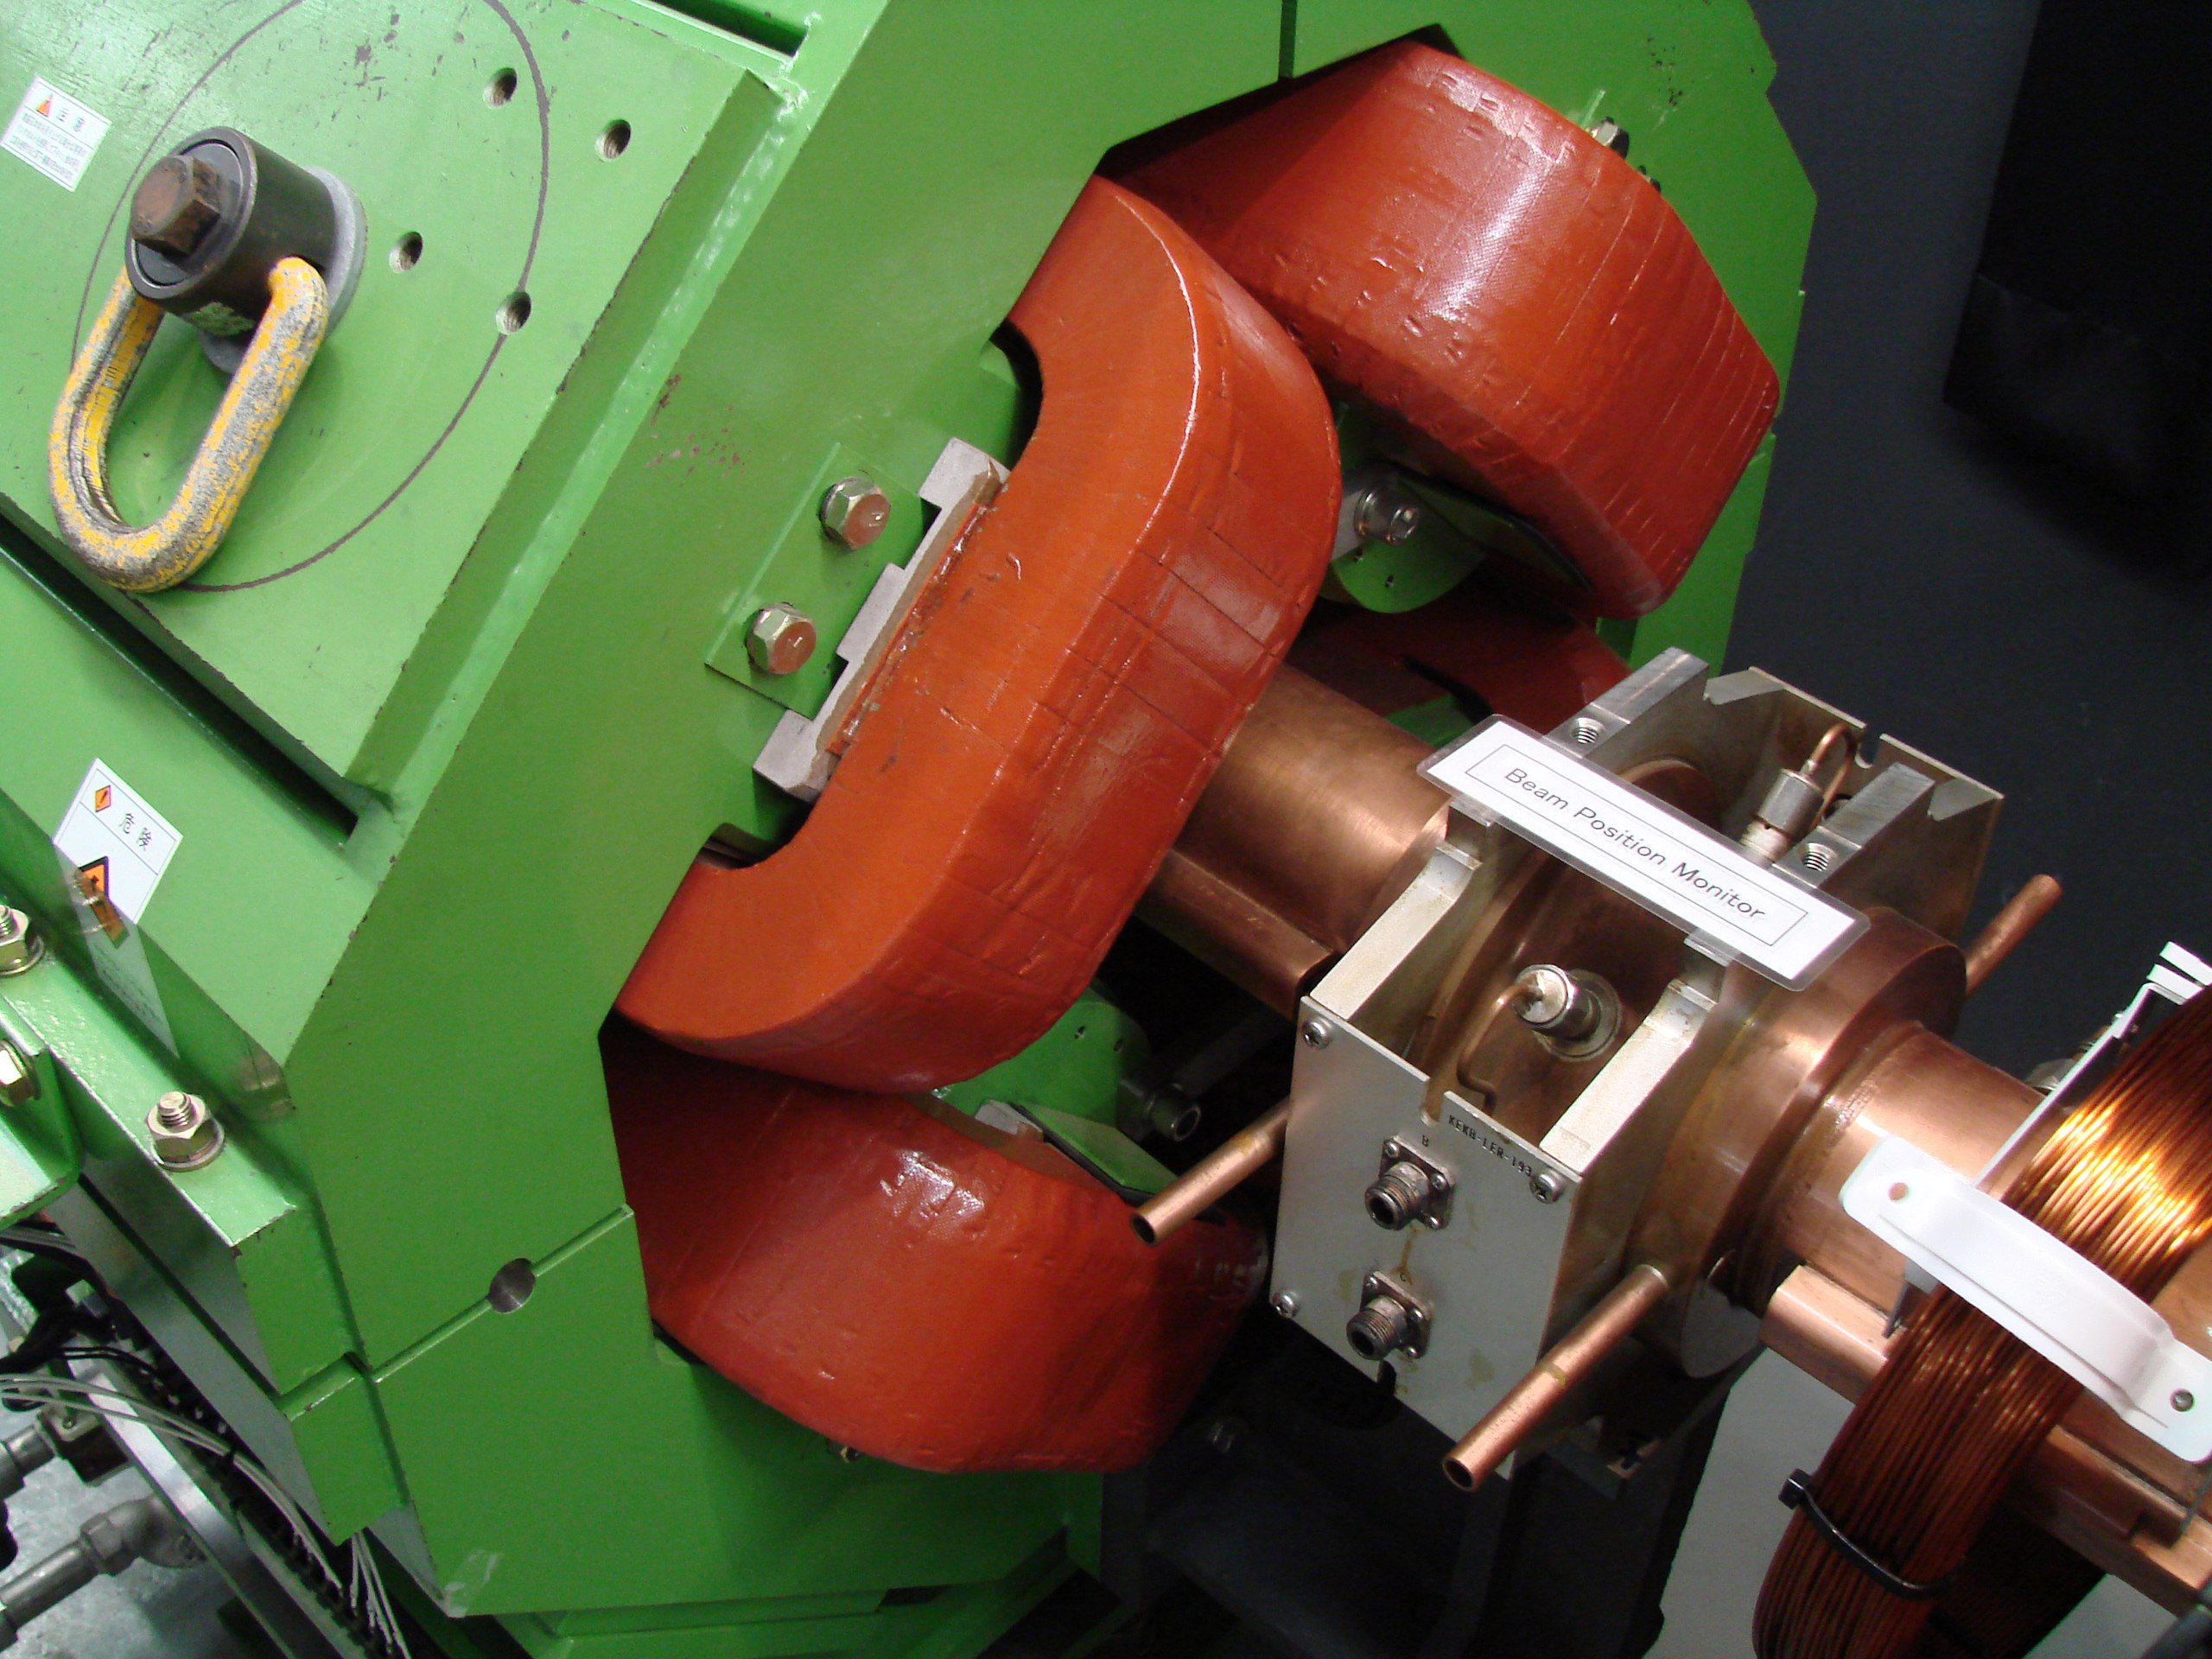
\includegraphics[width=0.7\textwidth]{quadrupole}
        \end{centering}
    \end{figure}
\end{frame}
\begin{frame}
    \begin{figure}
        \begin{centering}
            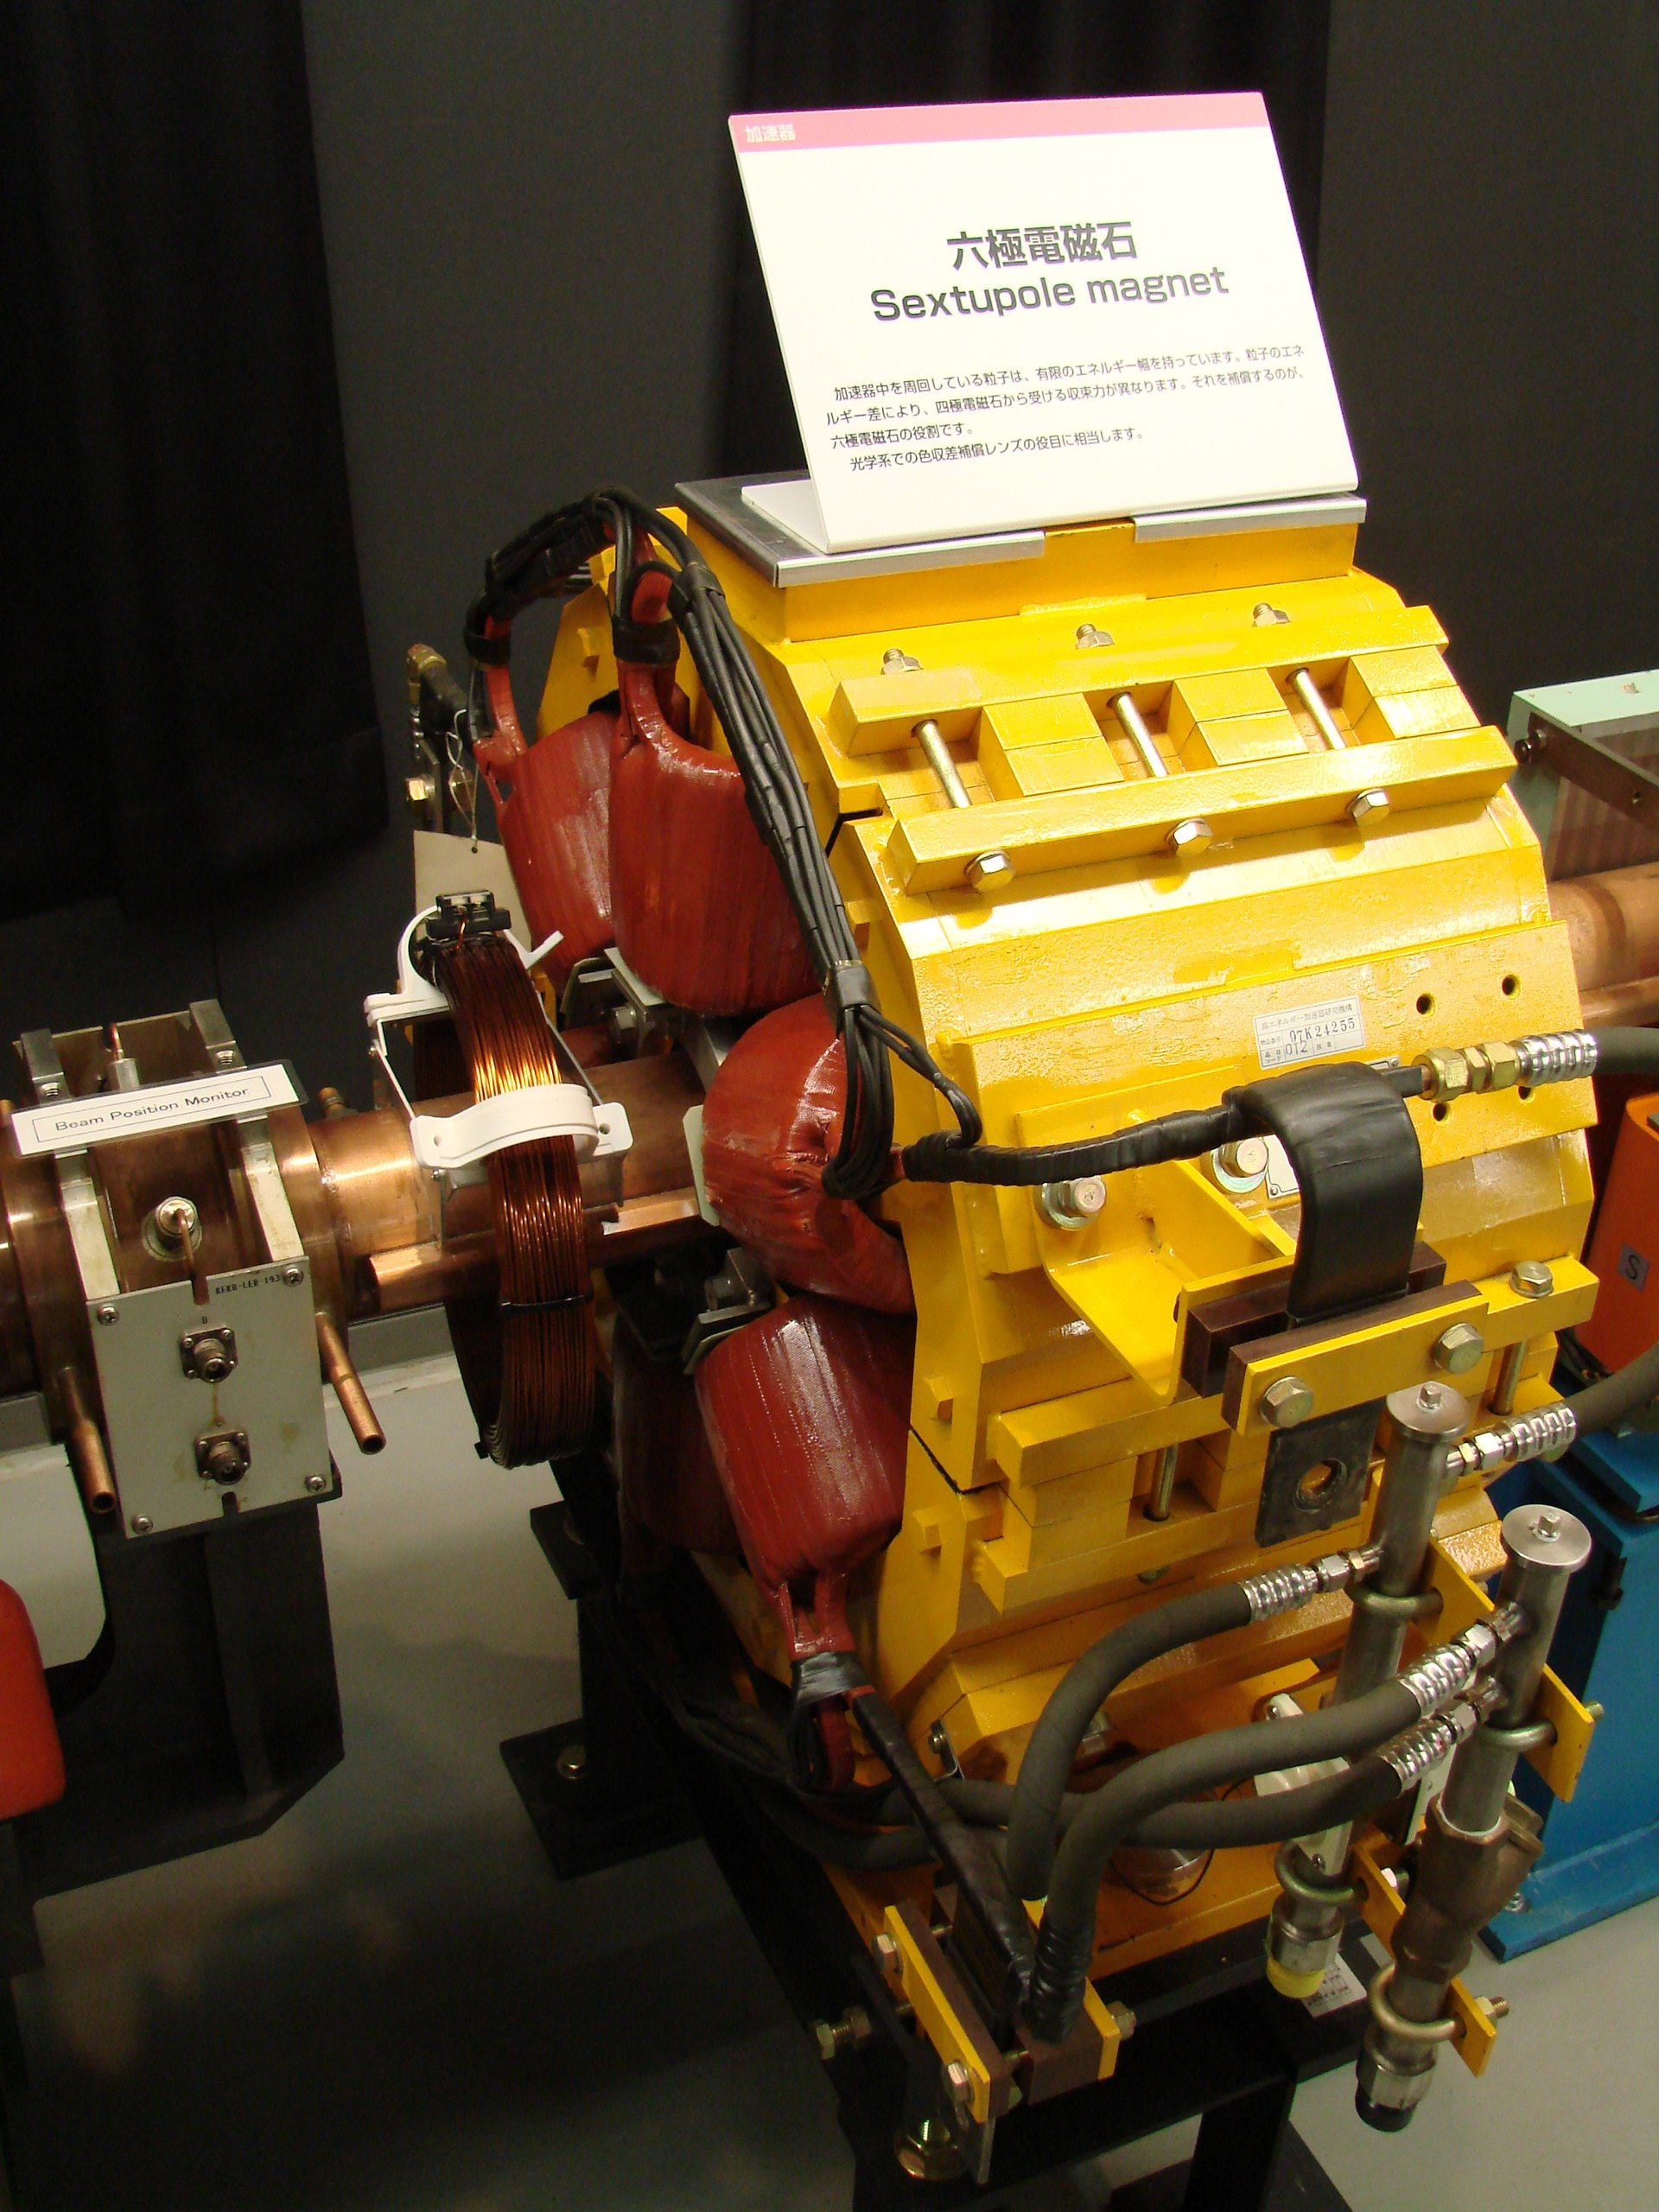
\includegraphics[width=0.7\textwidth]{sextupole}
        \end{centering}
    \end{figure}
\end{frame}

\begin{frame}
    \frametitle{Электрон-позитронный коллайдер}
    \begin{figure}
        \begin{centering}
            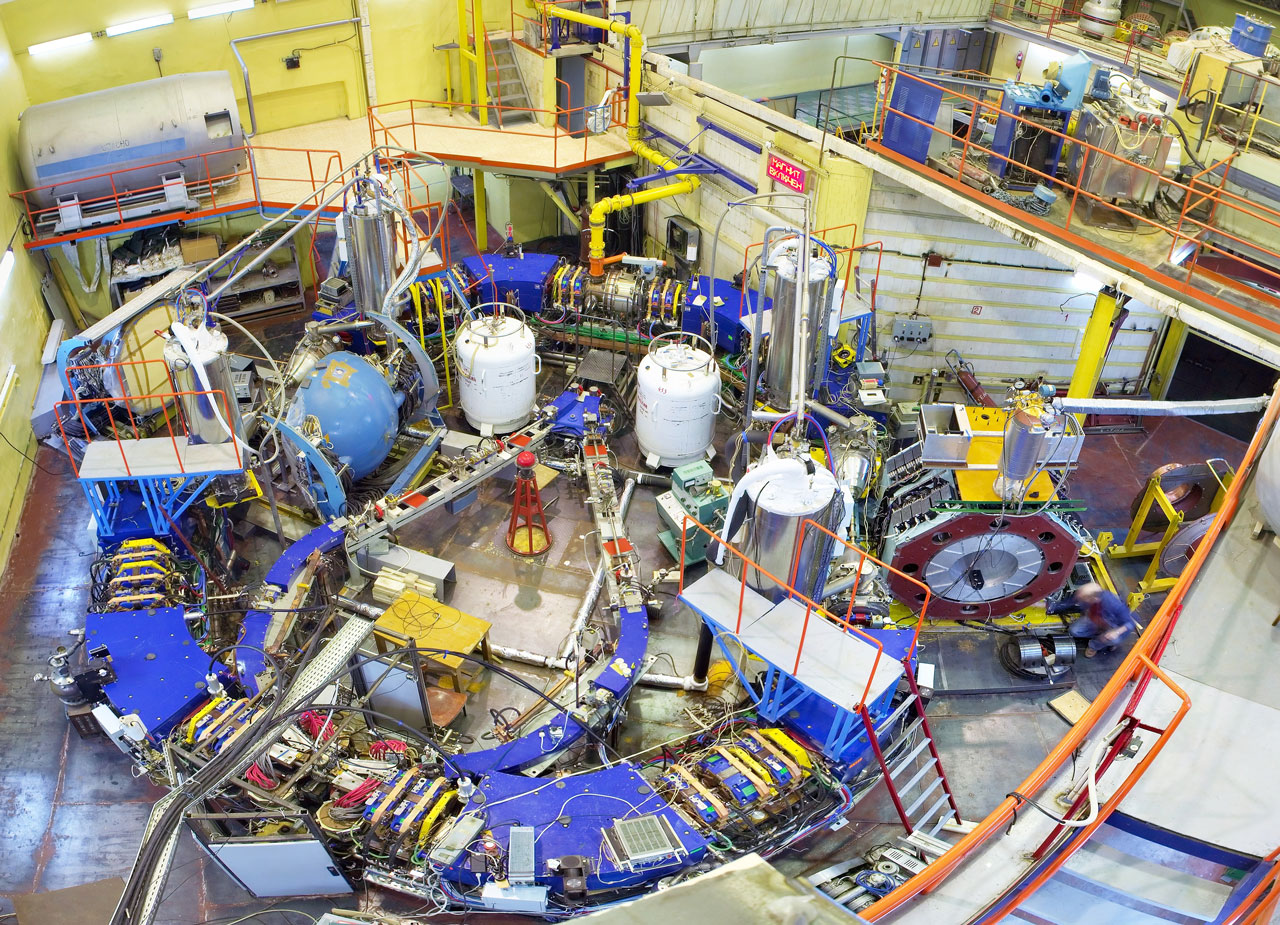
\includegraphics[width=0.7\textwidth]{vepp2}
        \end{centering}
    \end{figure}
\end{frame}

\subsection{Детекторы}
\begin{frame}
    \frametitle{Сферический детектор}
    \begin{figure}
        \begin{centering}
            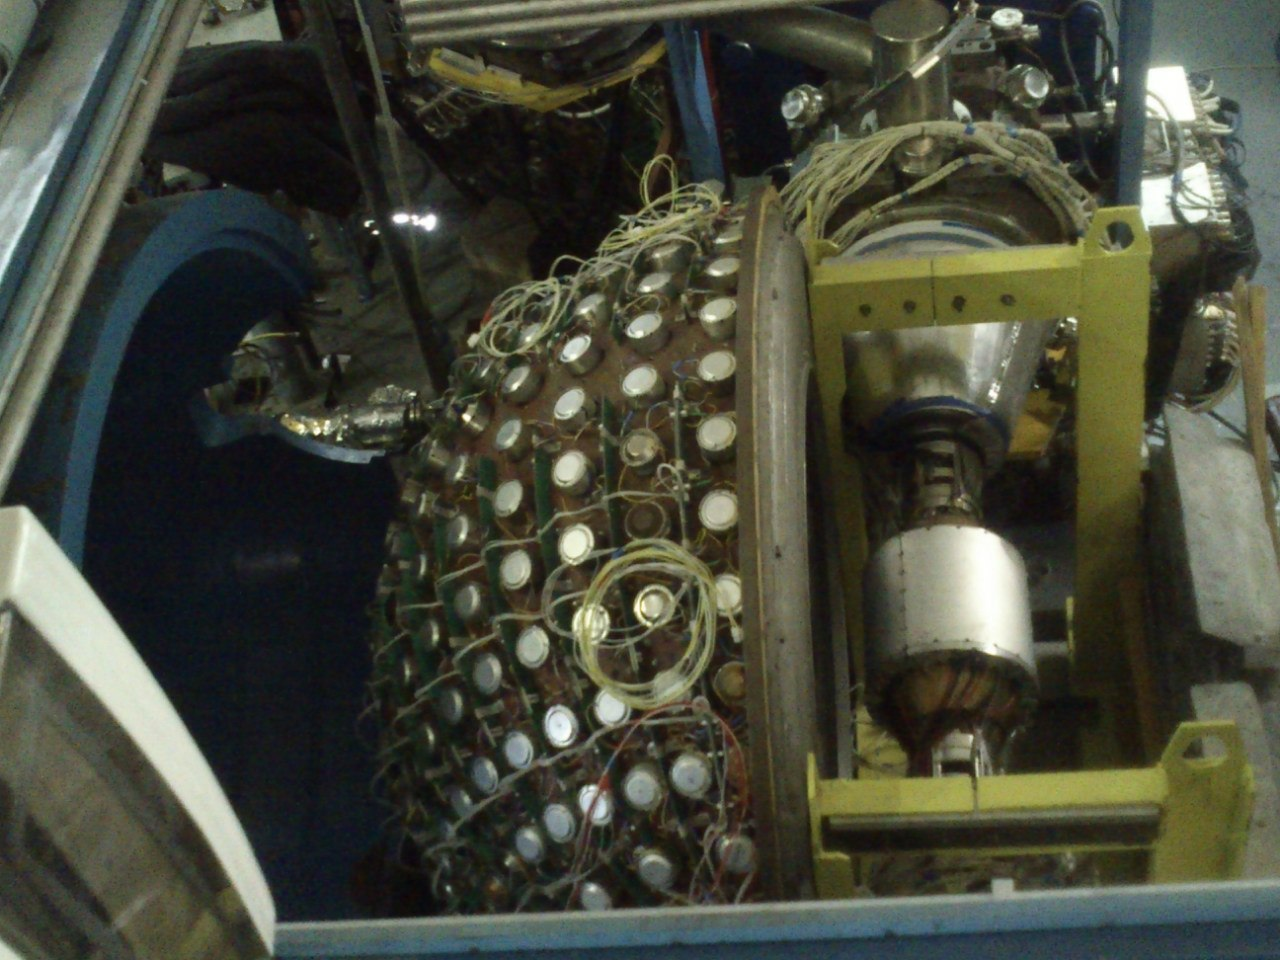
\includegraphics[width=0.7\textwidth]{snd}
        \end{centering}
    \end{figure}
\end{frame}
\begin{frame}
    \frametitle{Сферический детектор}
    \begin{figure}
        \begin{centering}
            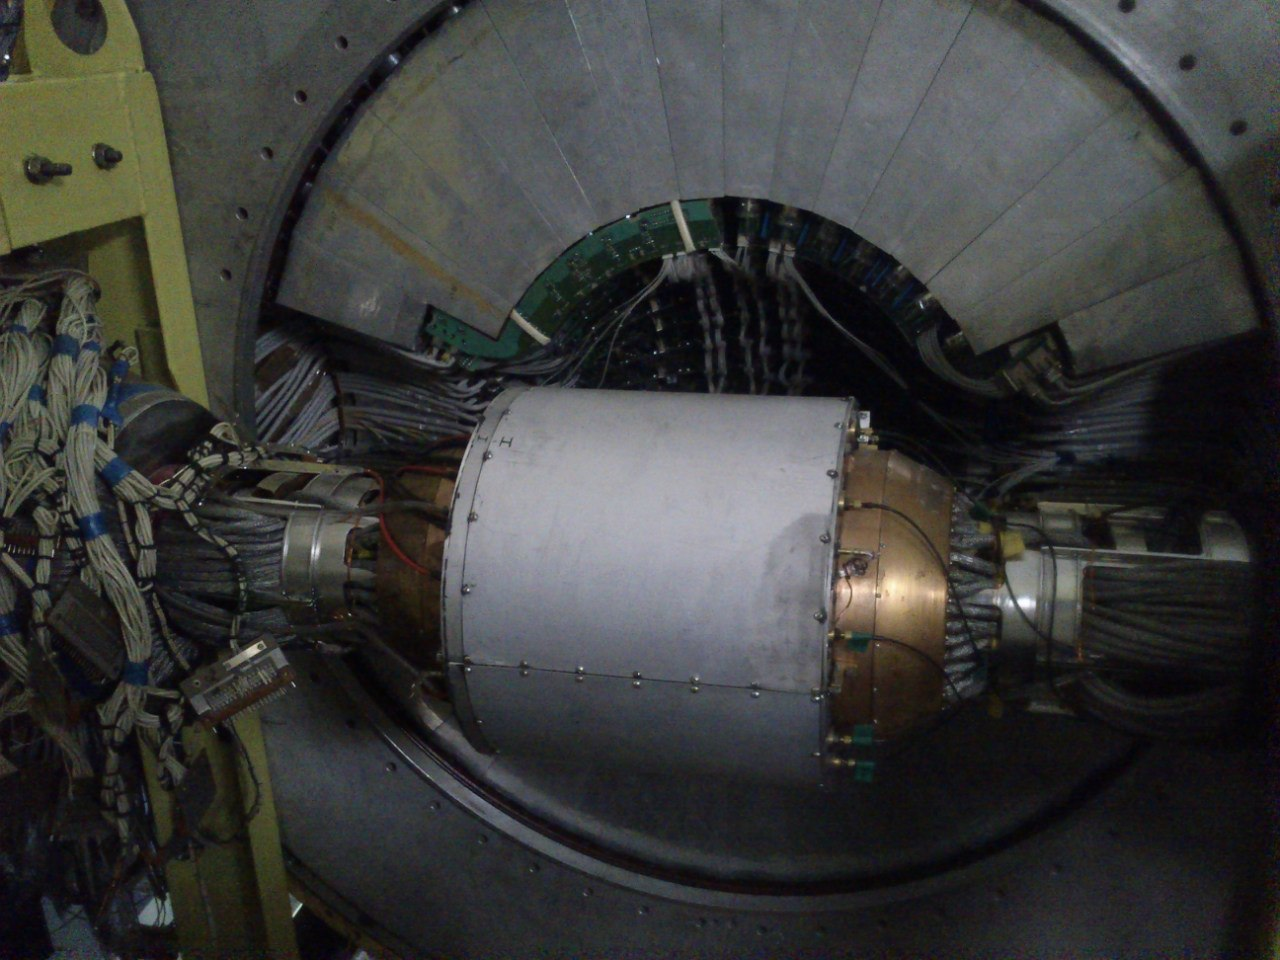
\includegraphics[width=0.7\textwidth]{snd-1st-half}
        \end{centering}
    \end{figure}
\end{frame}
\begin{frame}
    \frametitle{Сферический детектор}
    \begin{figure}
        \begin{centering}
            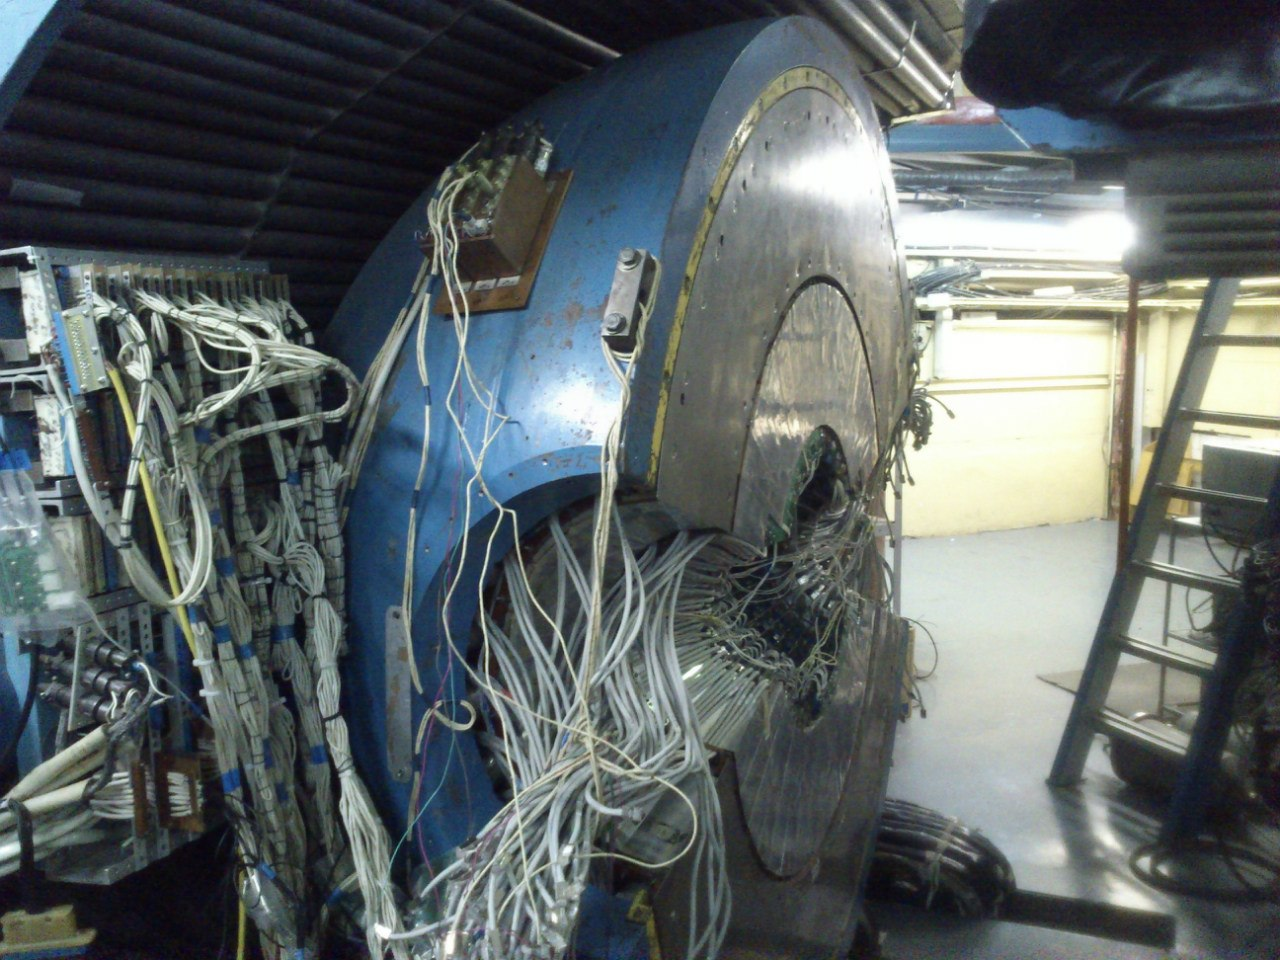
\includegraphics[width=0.7\textwidth]{snd-2nd-half}
        \end{centering}
    \end{figure}
\end{frame}

\subsection{B-фабрика}
\begin{frame}
    \frametitle{Японская фабрика B-мезонов}
    \begin{figure}
        \begin{centering}
            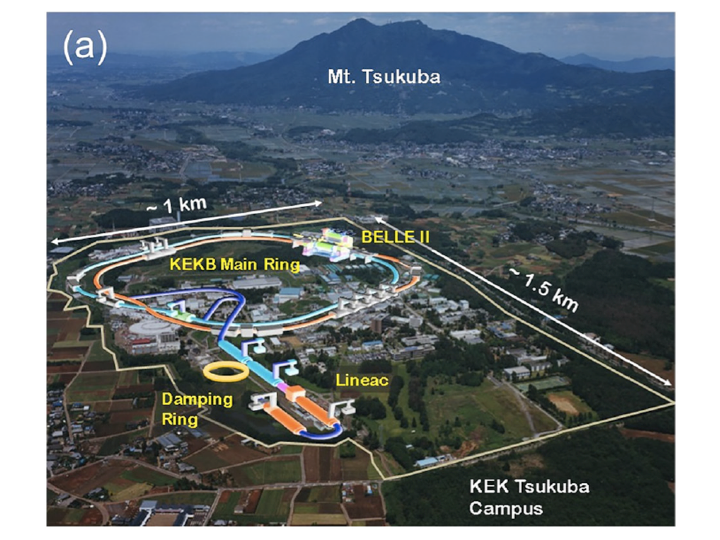
\includegraphics[width=0.7\textwidth]{kekb-tsukuba}
        \end{centering}
    \end{figure}
\end{frame}
\begin{frame}
    \frametitle{Точки выхода на поверхность}
    \begin{figure}
        \begin{centering}
            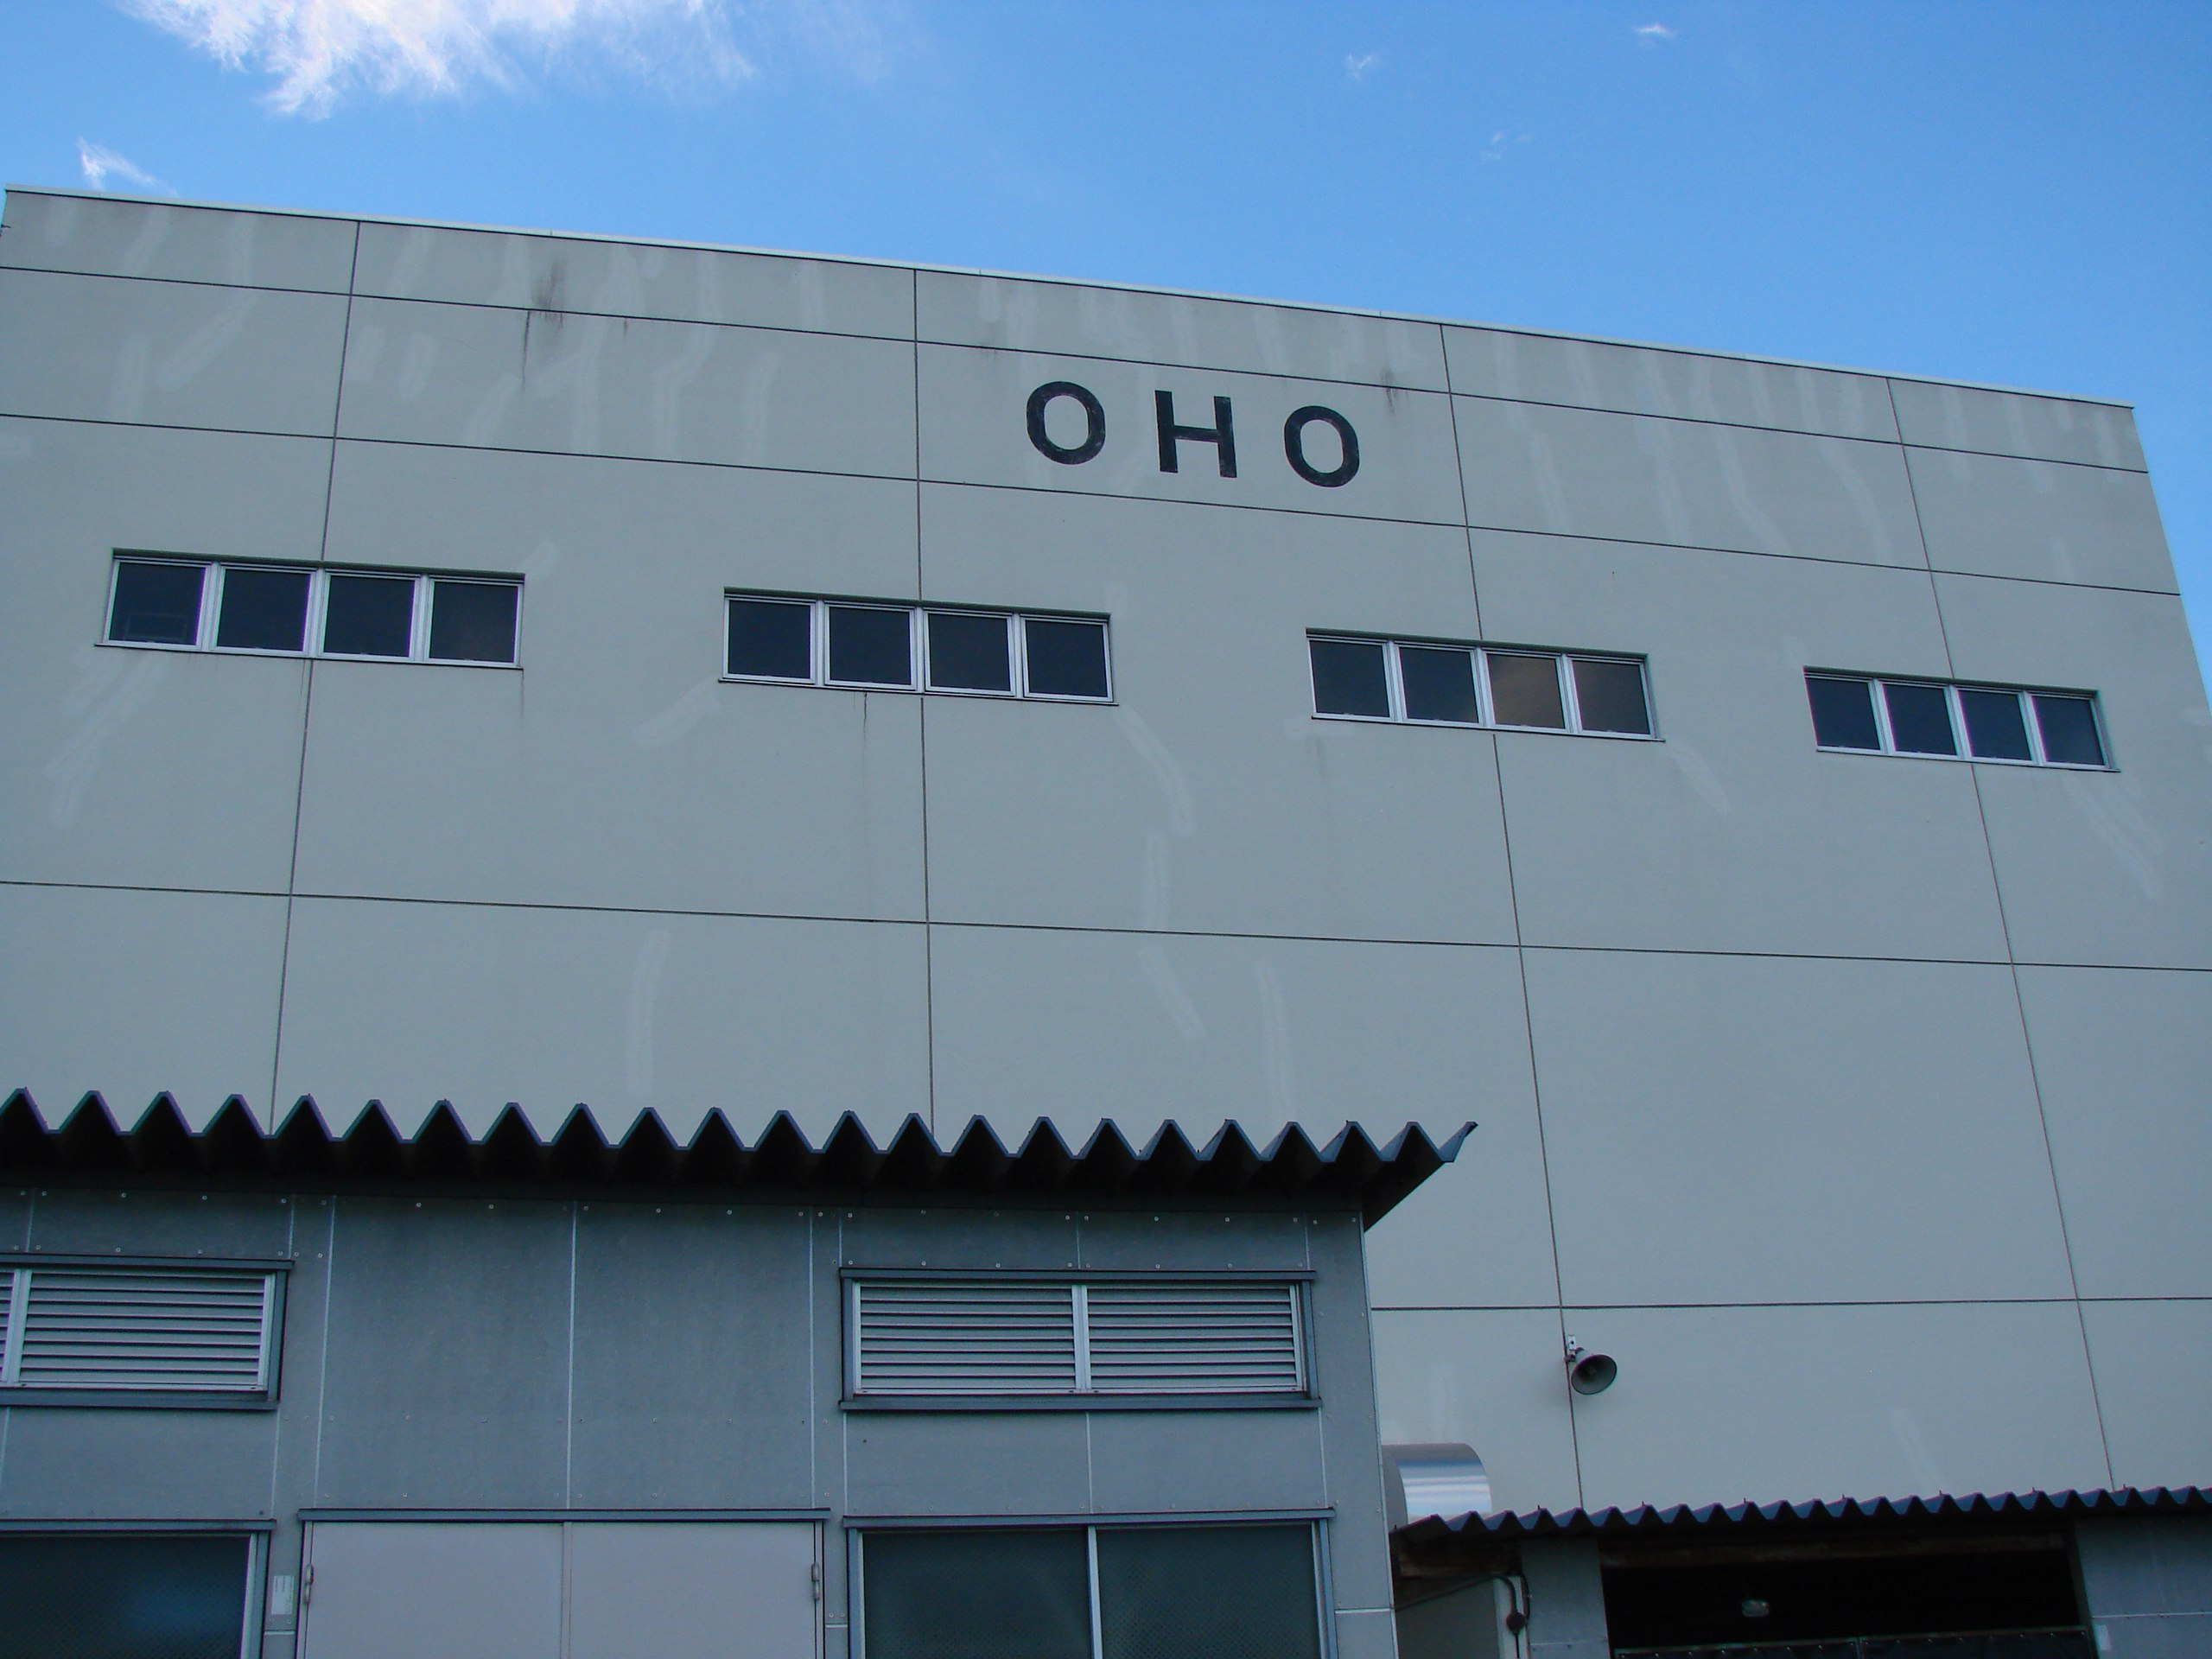
\includegraphics[width=0.7\textwidth]{oho}
        \end{centering}
    \end{figure}
\end{frame}
\begin{frame}
    \frametitle{Точки выхода на поверхность: детектор}
    \begin{figure}
        \begin{centering}
            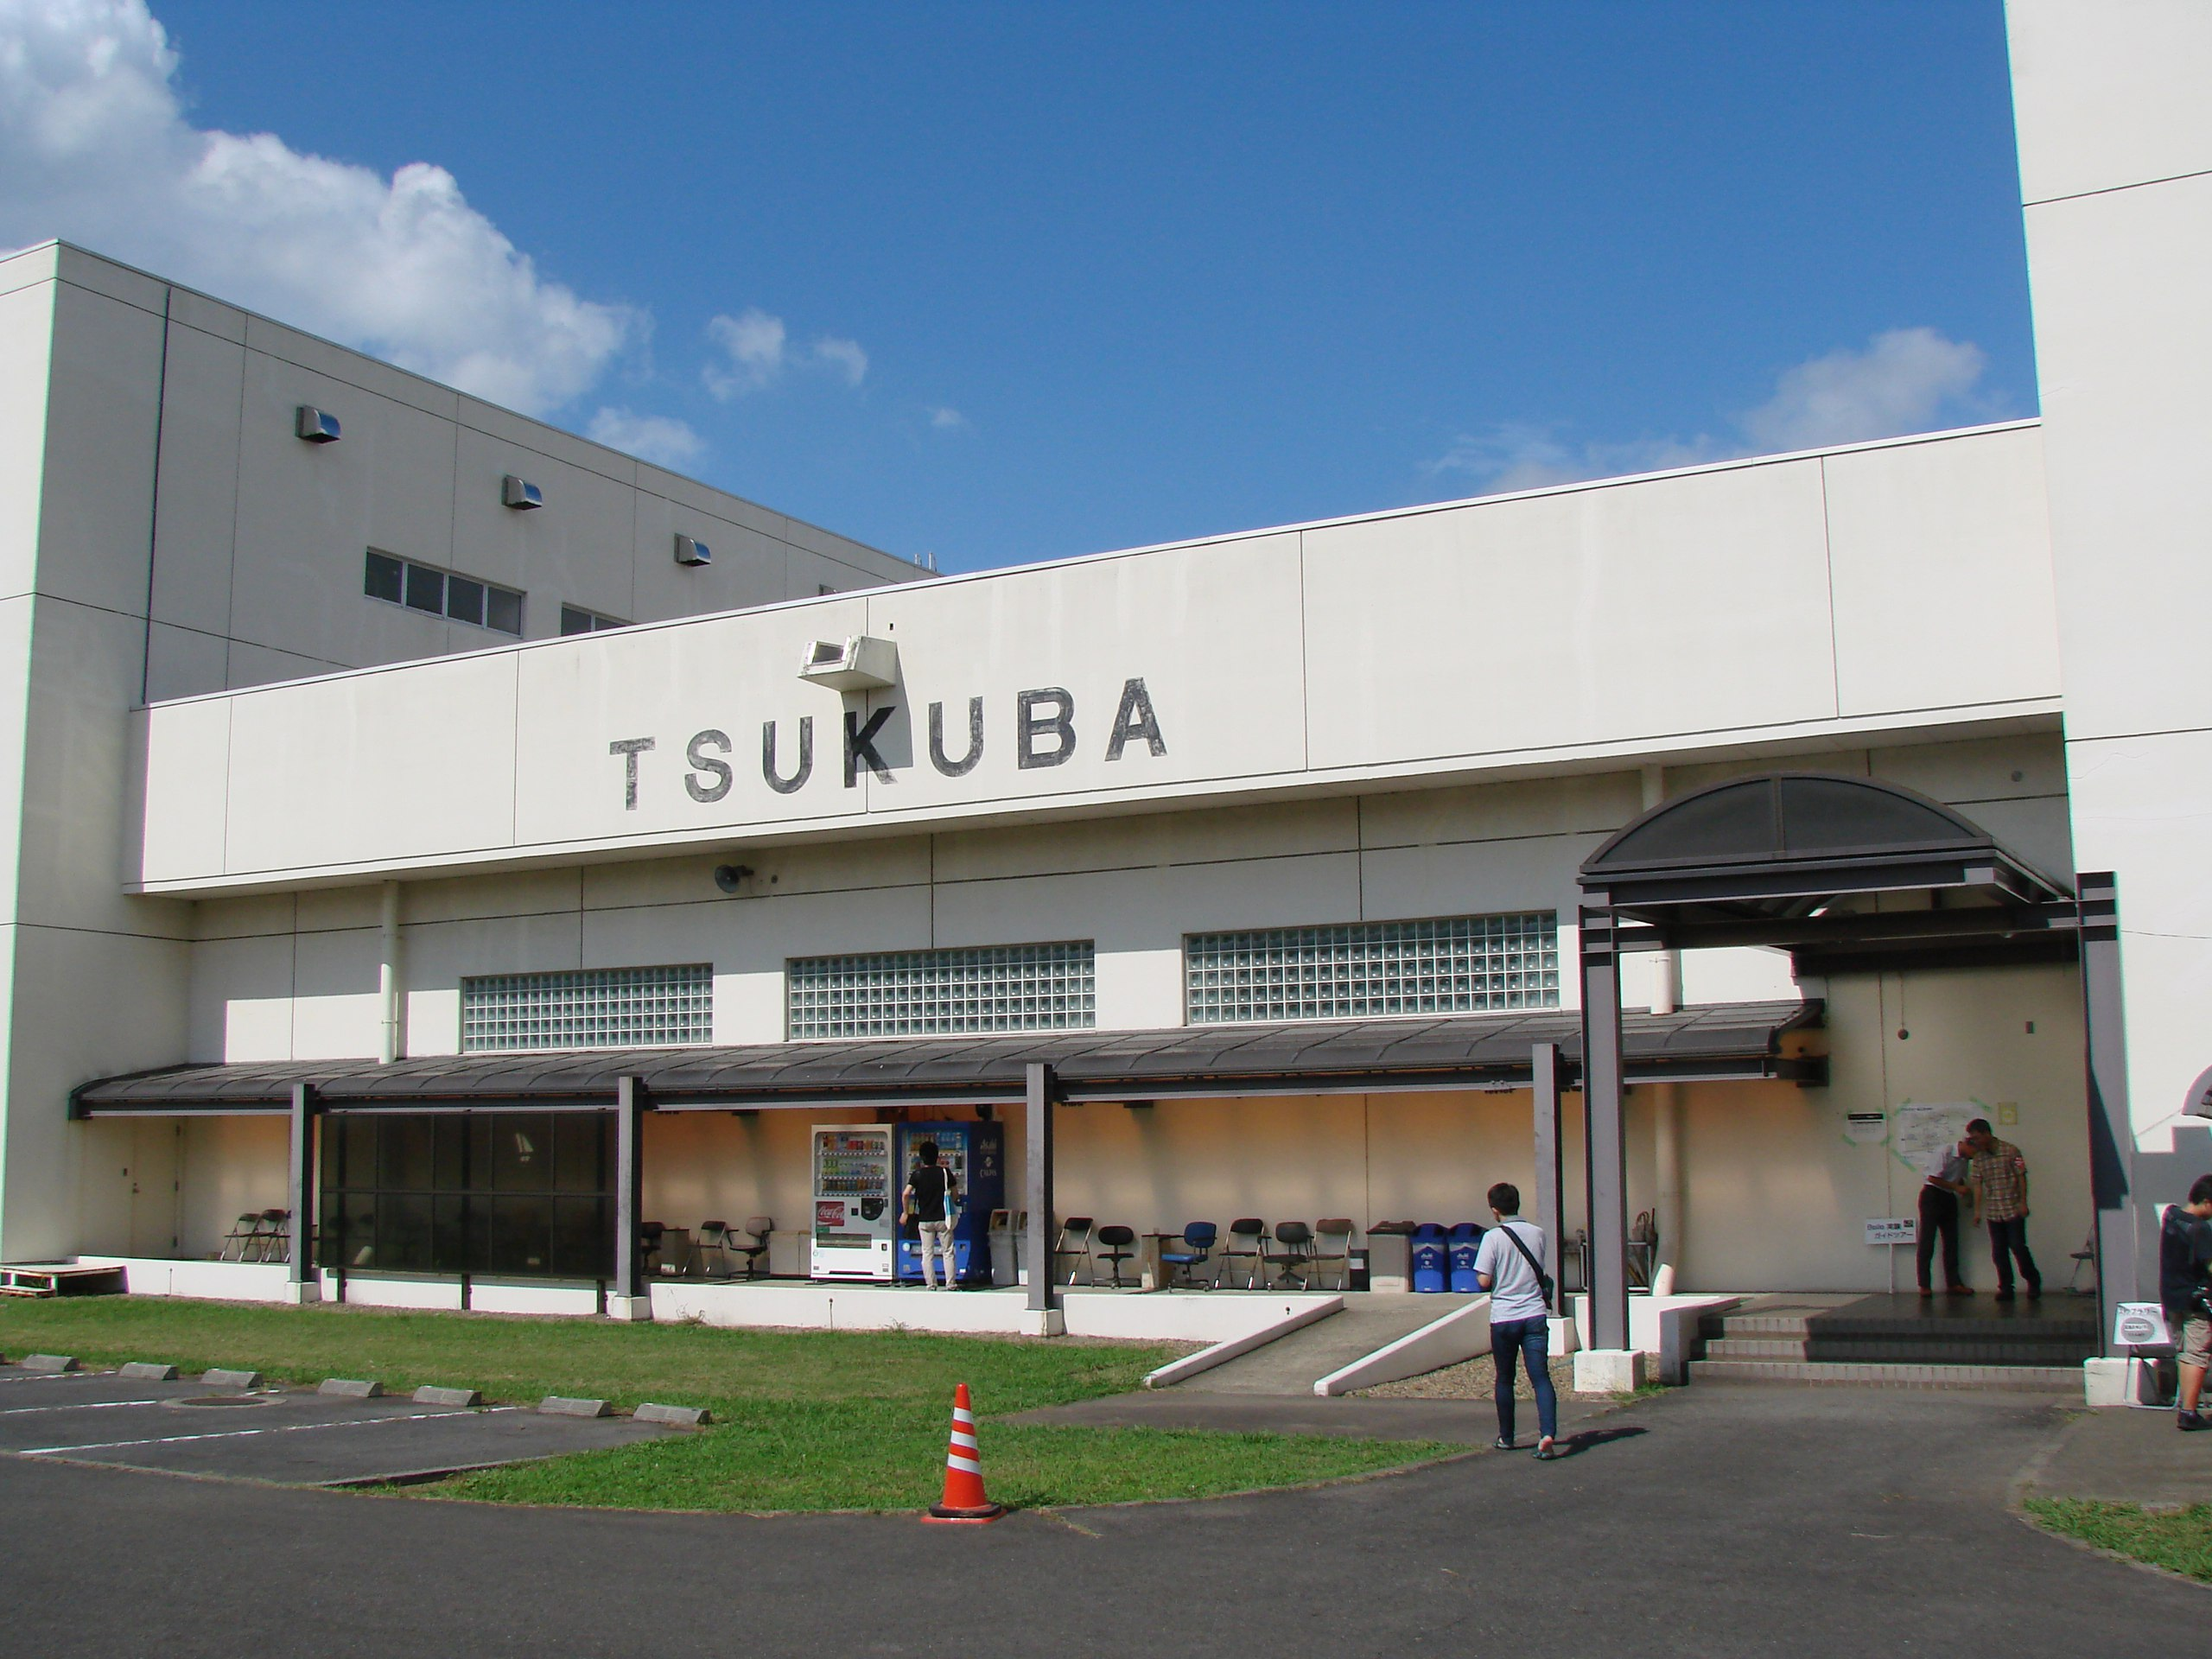
\includegraphics[width=0.7\textwidth]{tsukuba}
        \end{centering}
    \end{figure}
\end{frame}
\begin{frame}
    \frametitle{Детектор Белль 2 под землёй}
    \begin{figure}
        \begin{centering}
            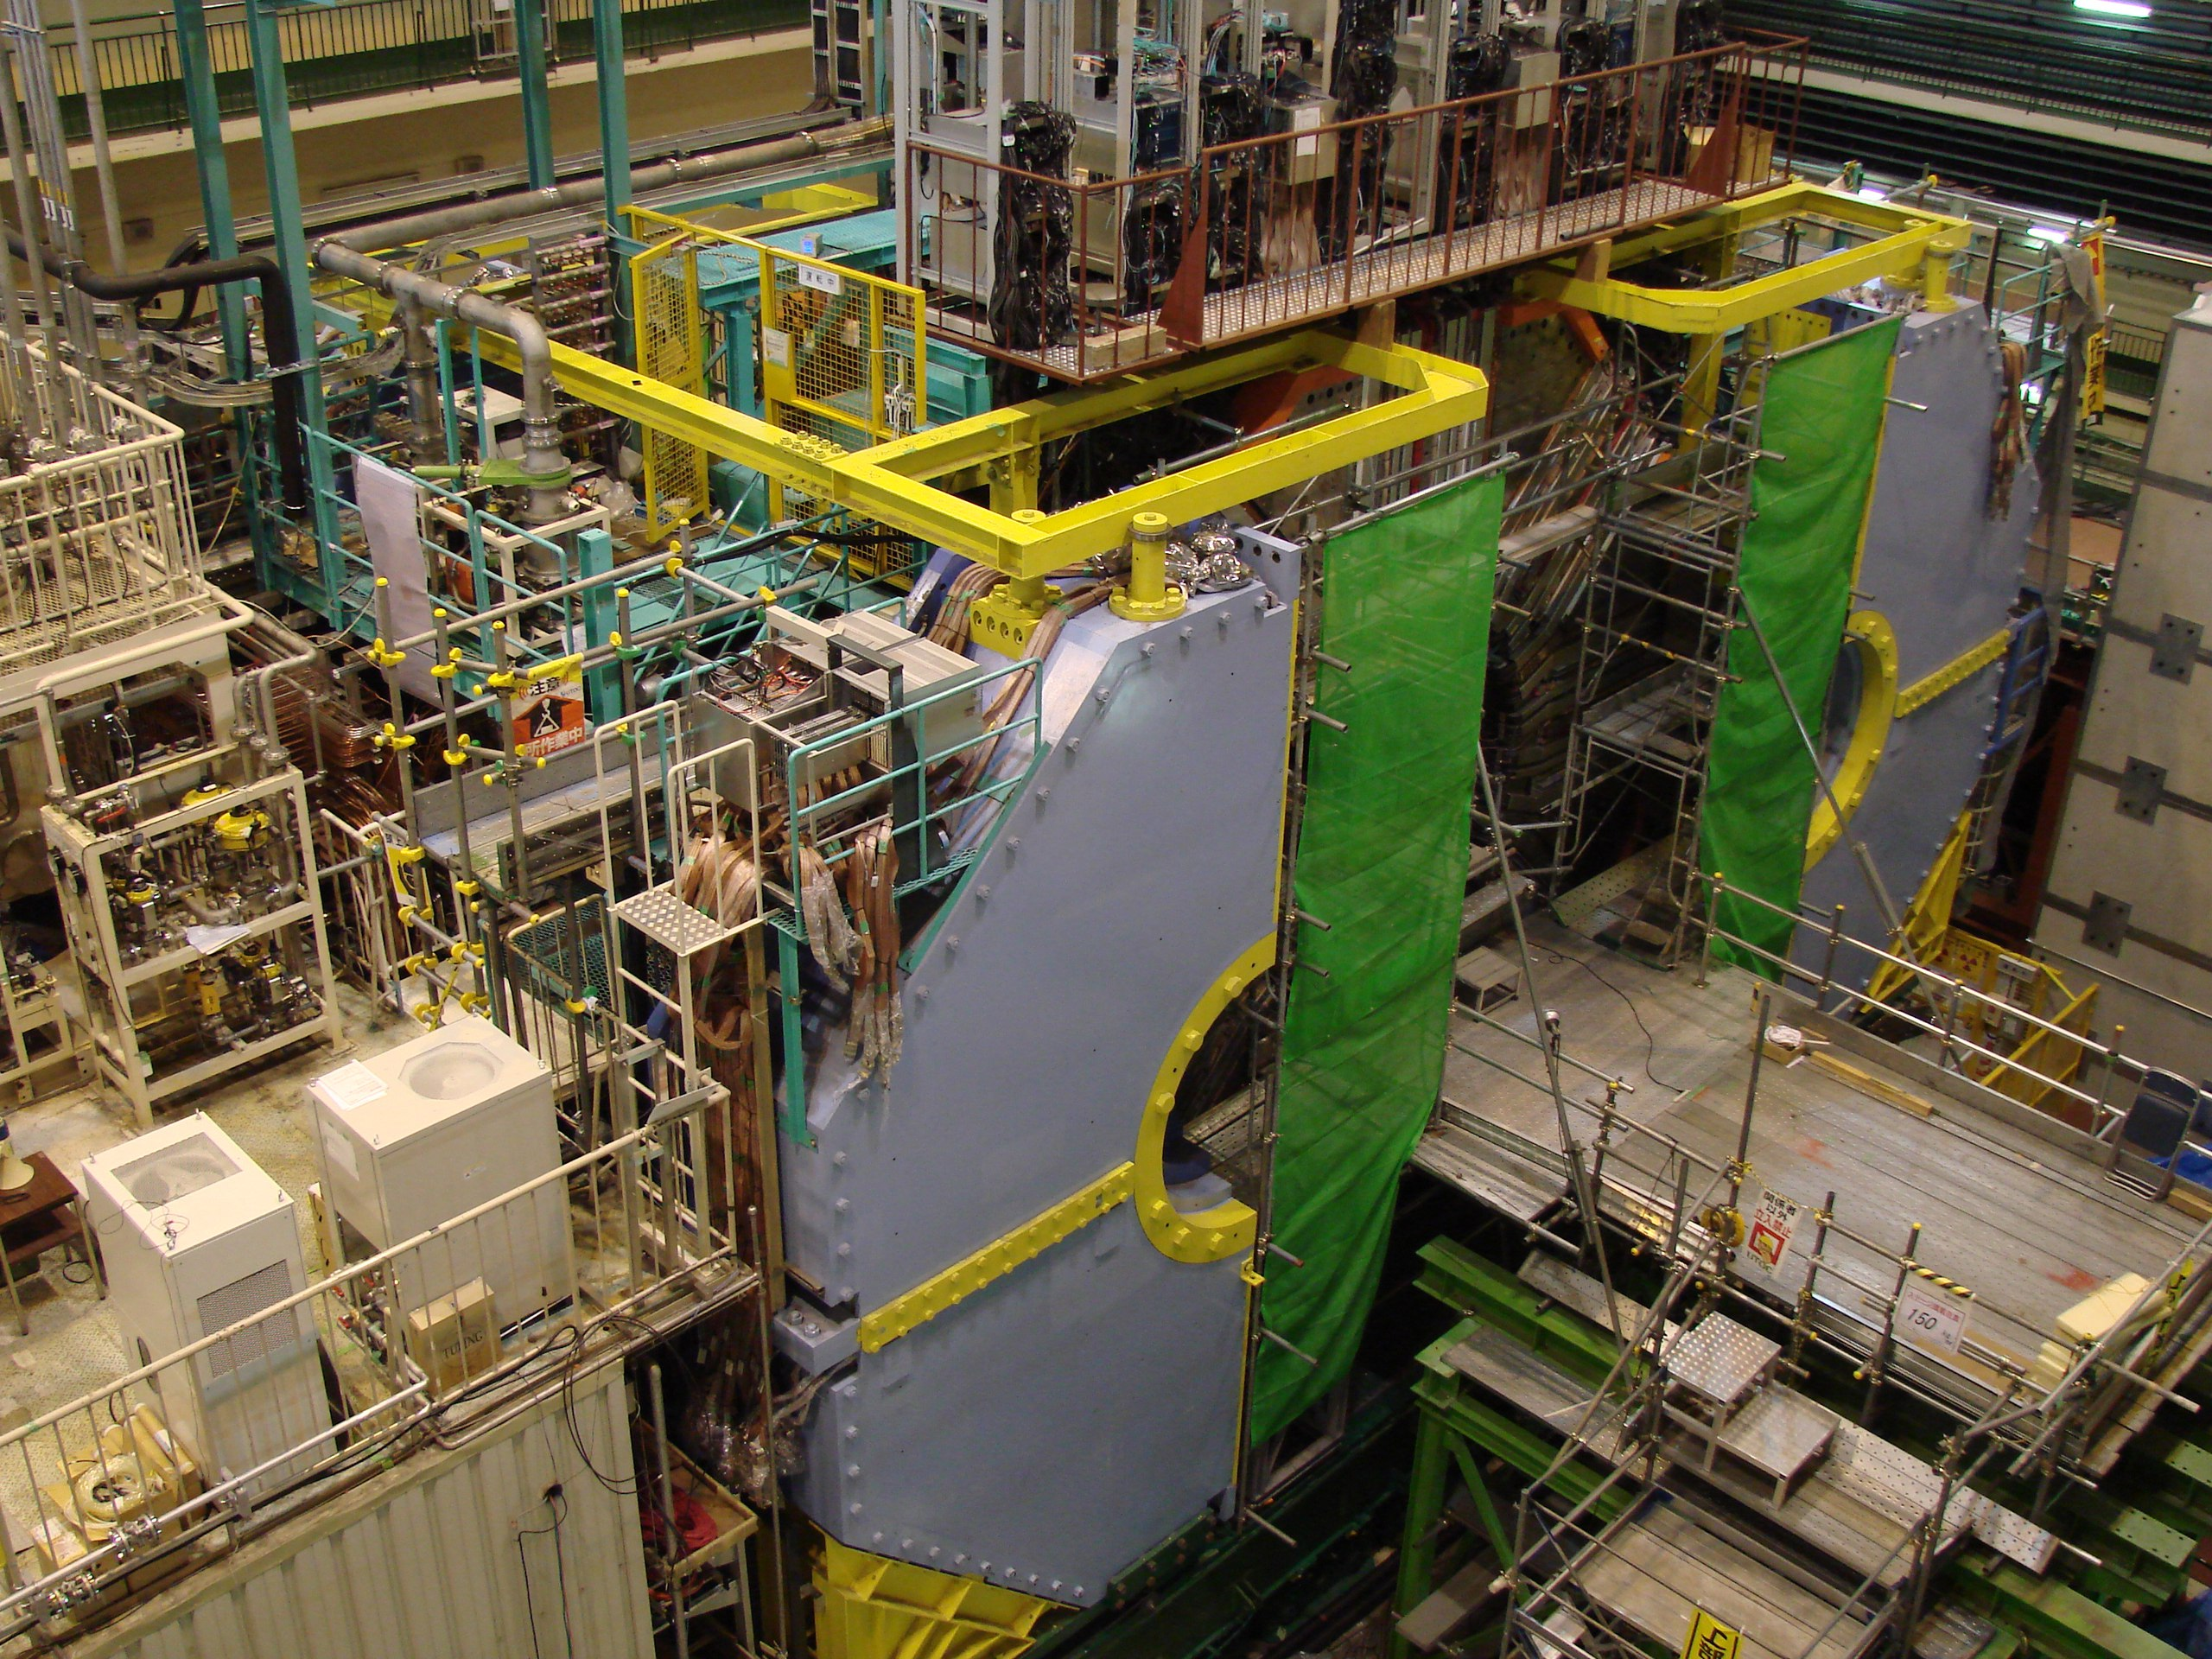
\includegraphics[width=0.7\textwidth]{belle2}
        \end{centering}
    \end{figure}
\end{frame}
\begin{frame}
    \frametitle{Детектор Белль 2 под землёй}
    \begin{figure}
        \begin{centering}
            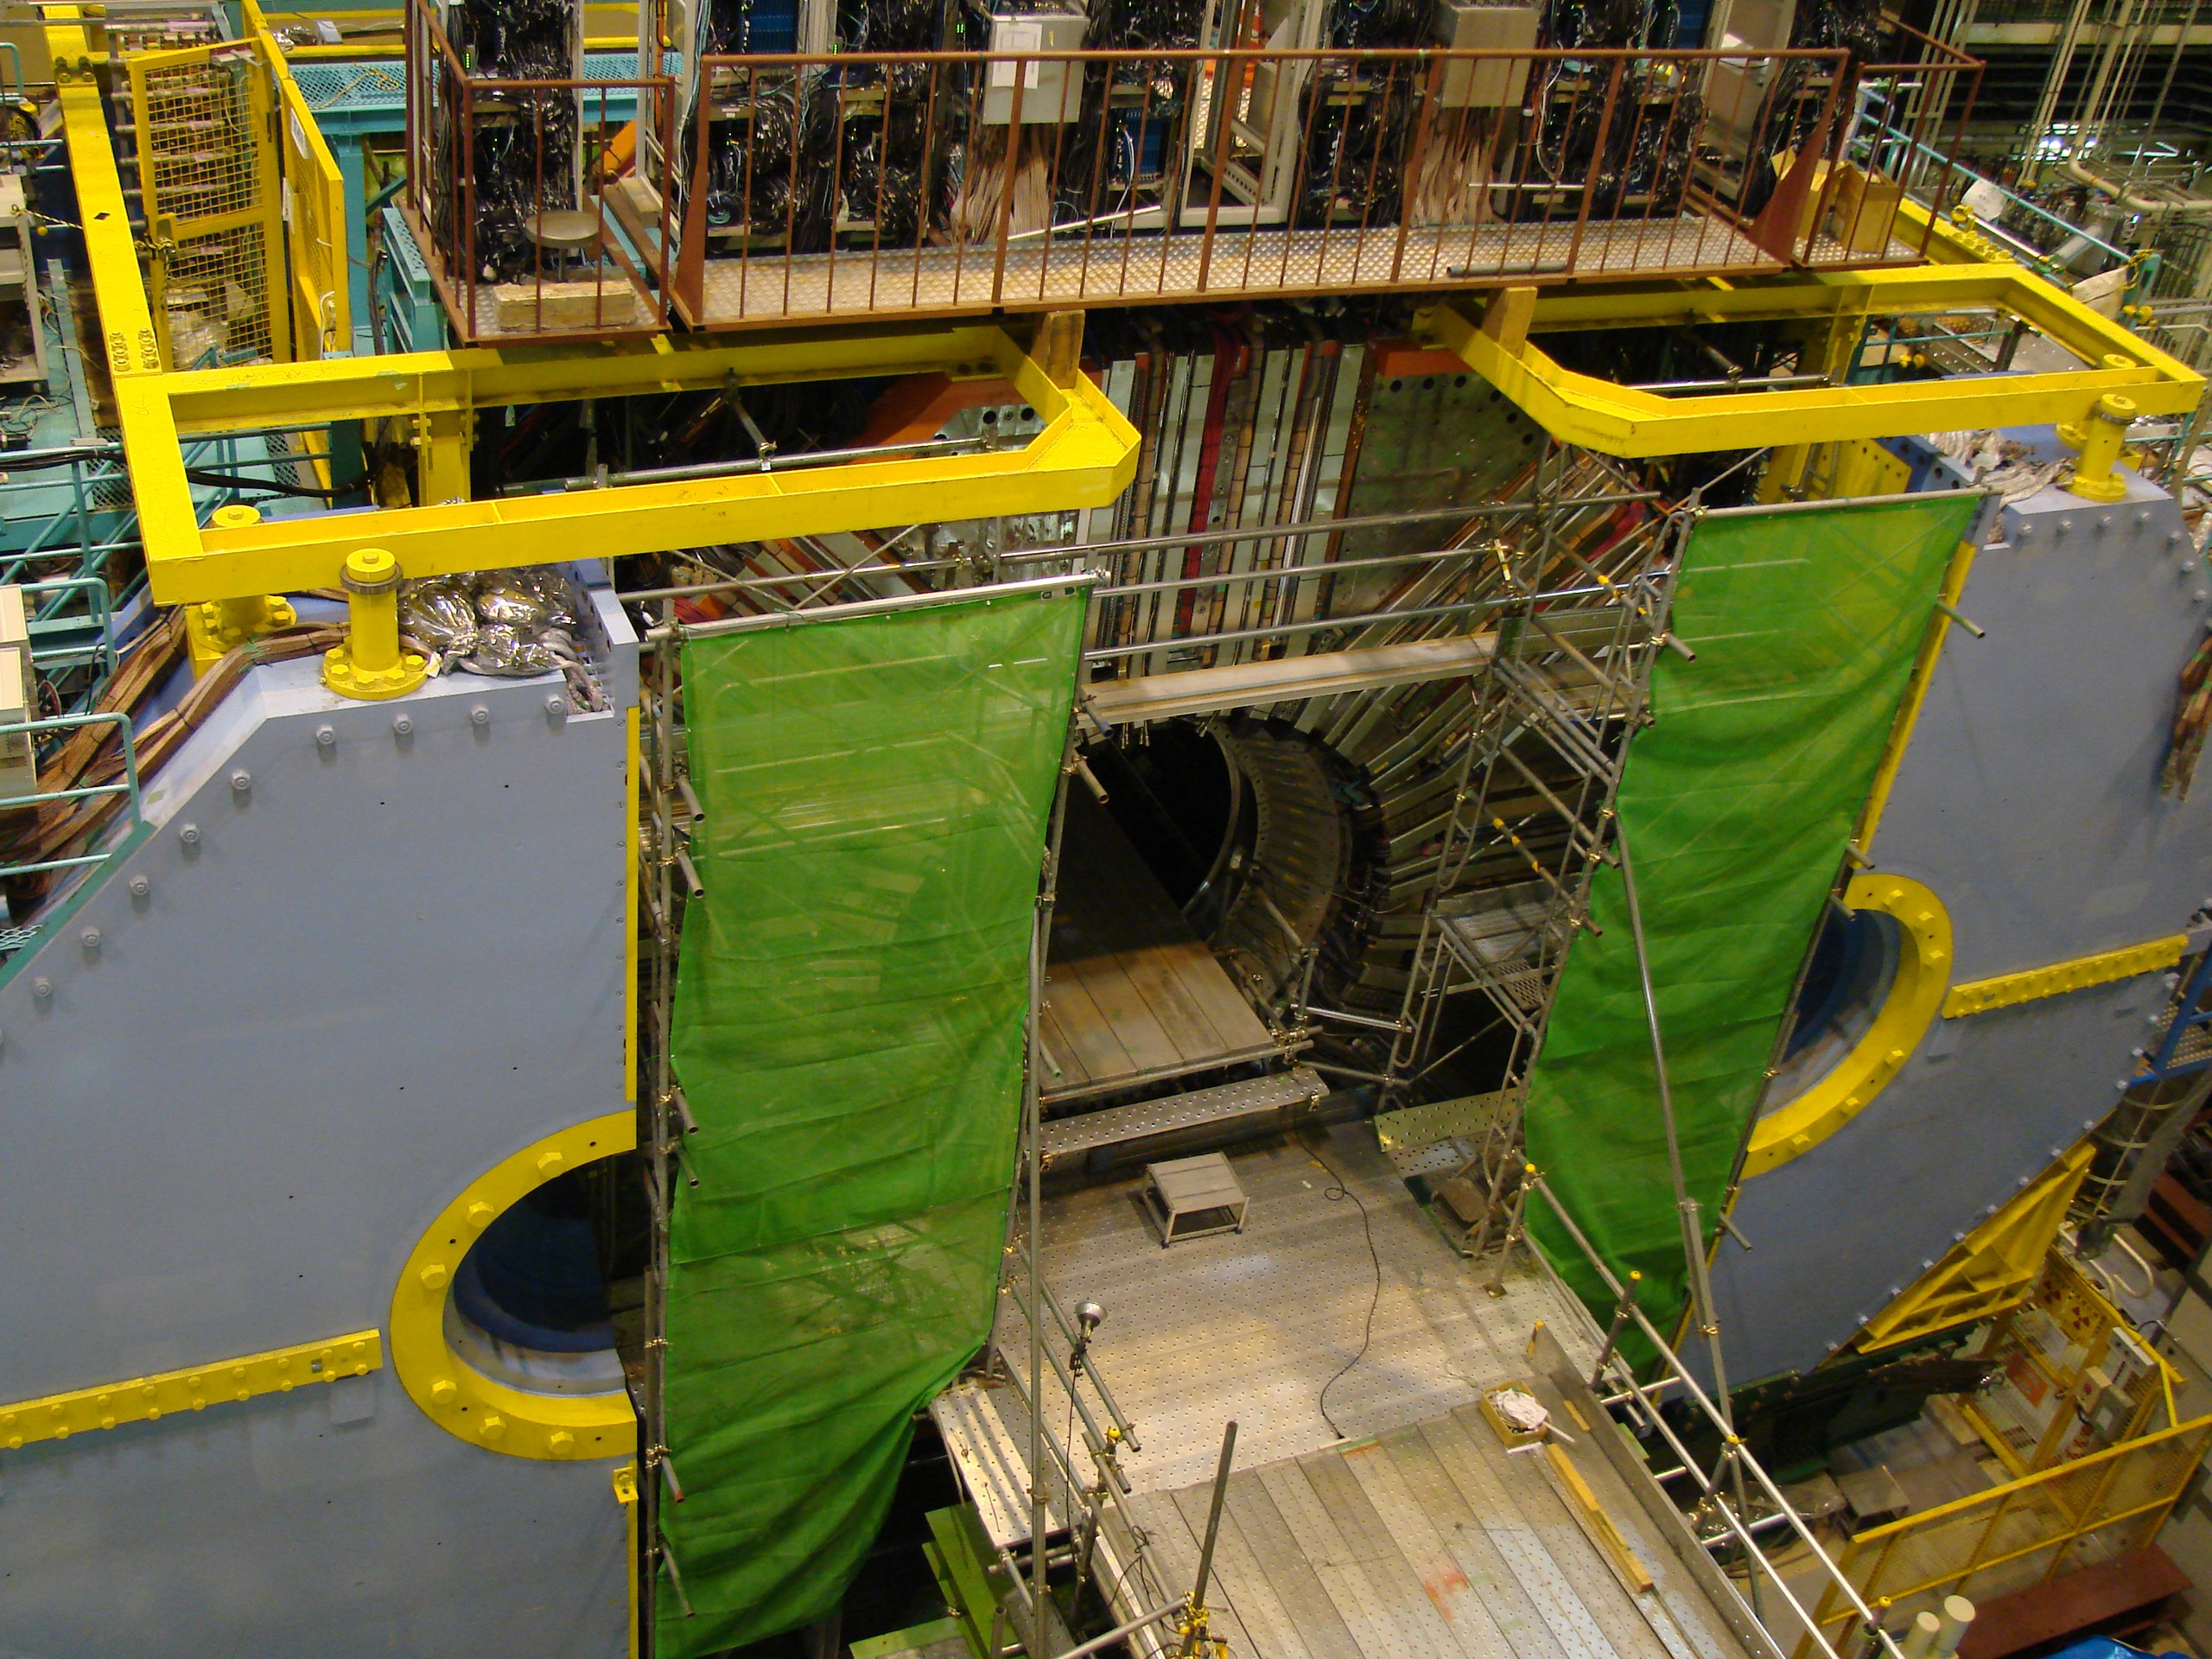
\includegraphics[width=0.7\textwidth]{belle2center}
        \end{centering}
    \end{figure}
\end{frame}
\begin{frame}
    \frametitle{Схема детектора Belle II}
    \begin{figure}
        \begin{centering}
            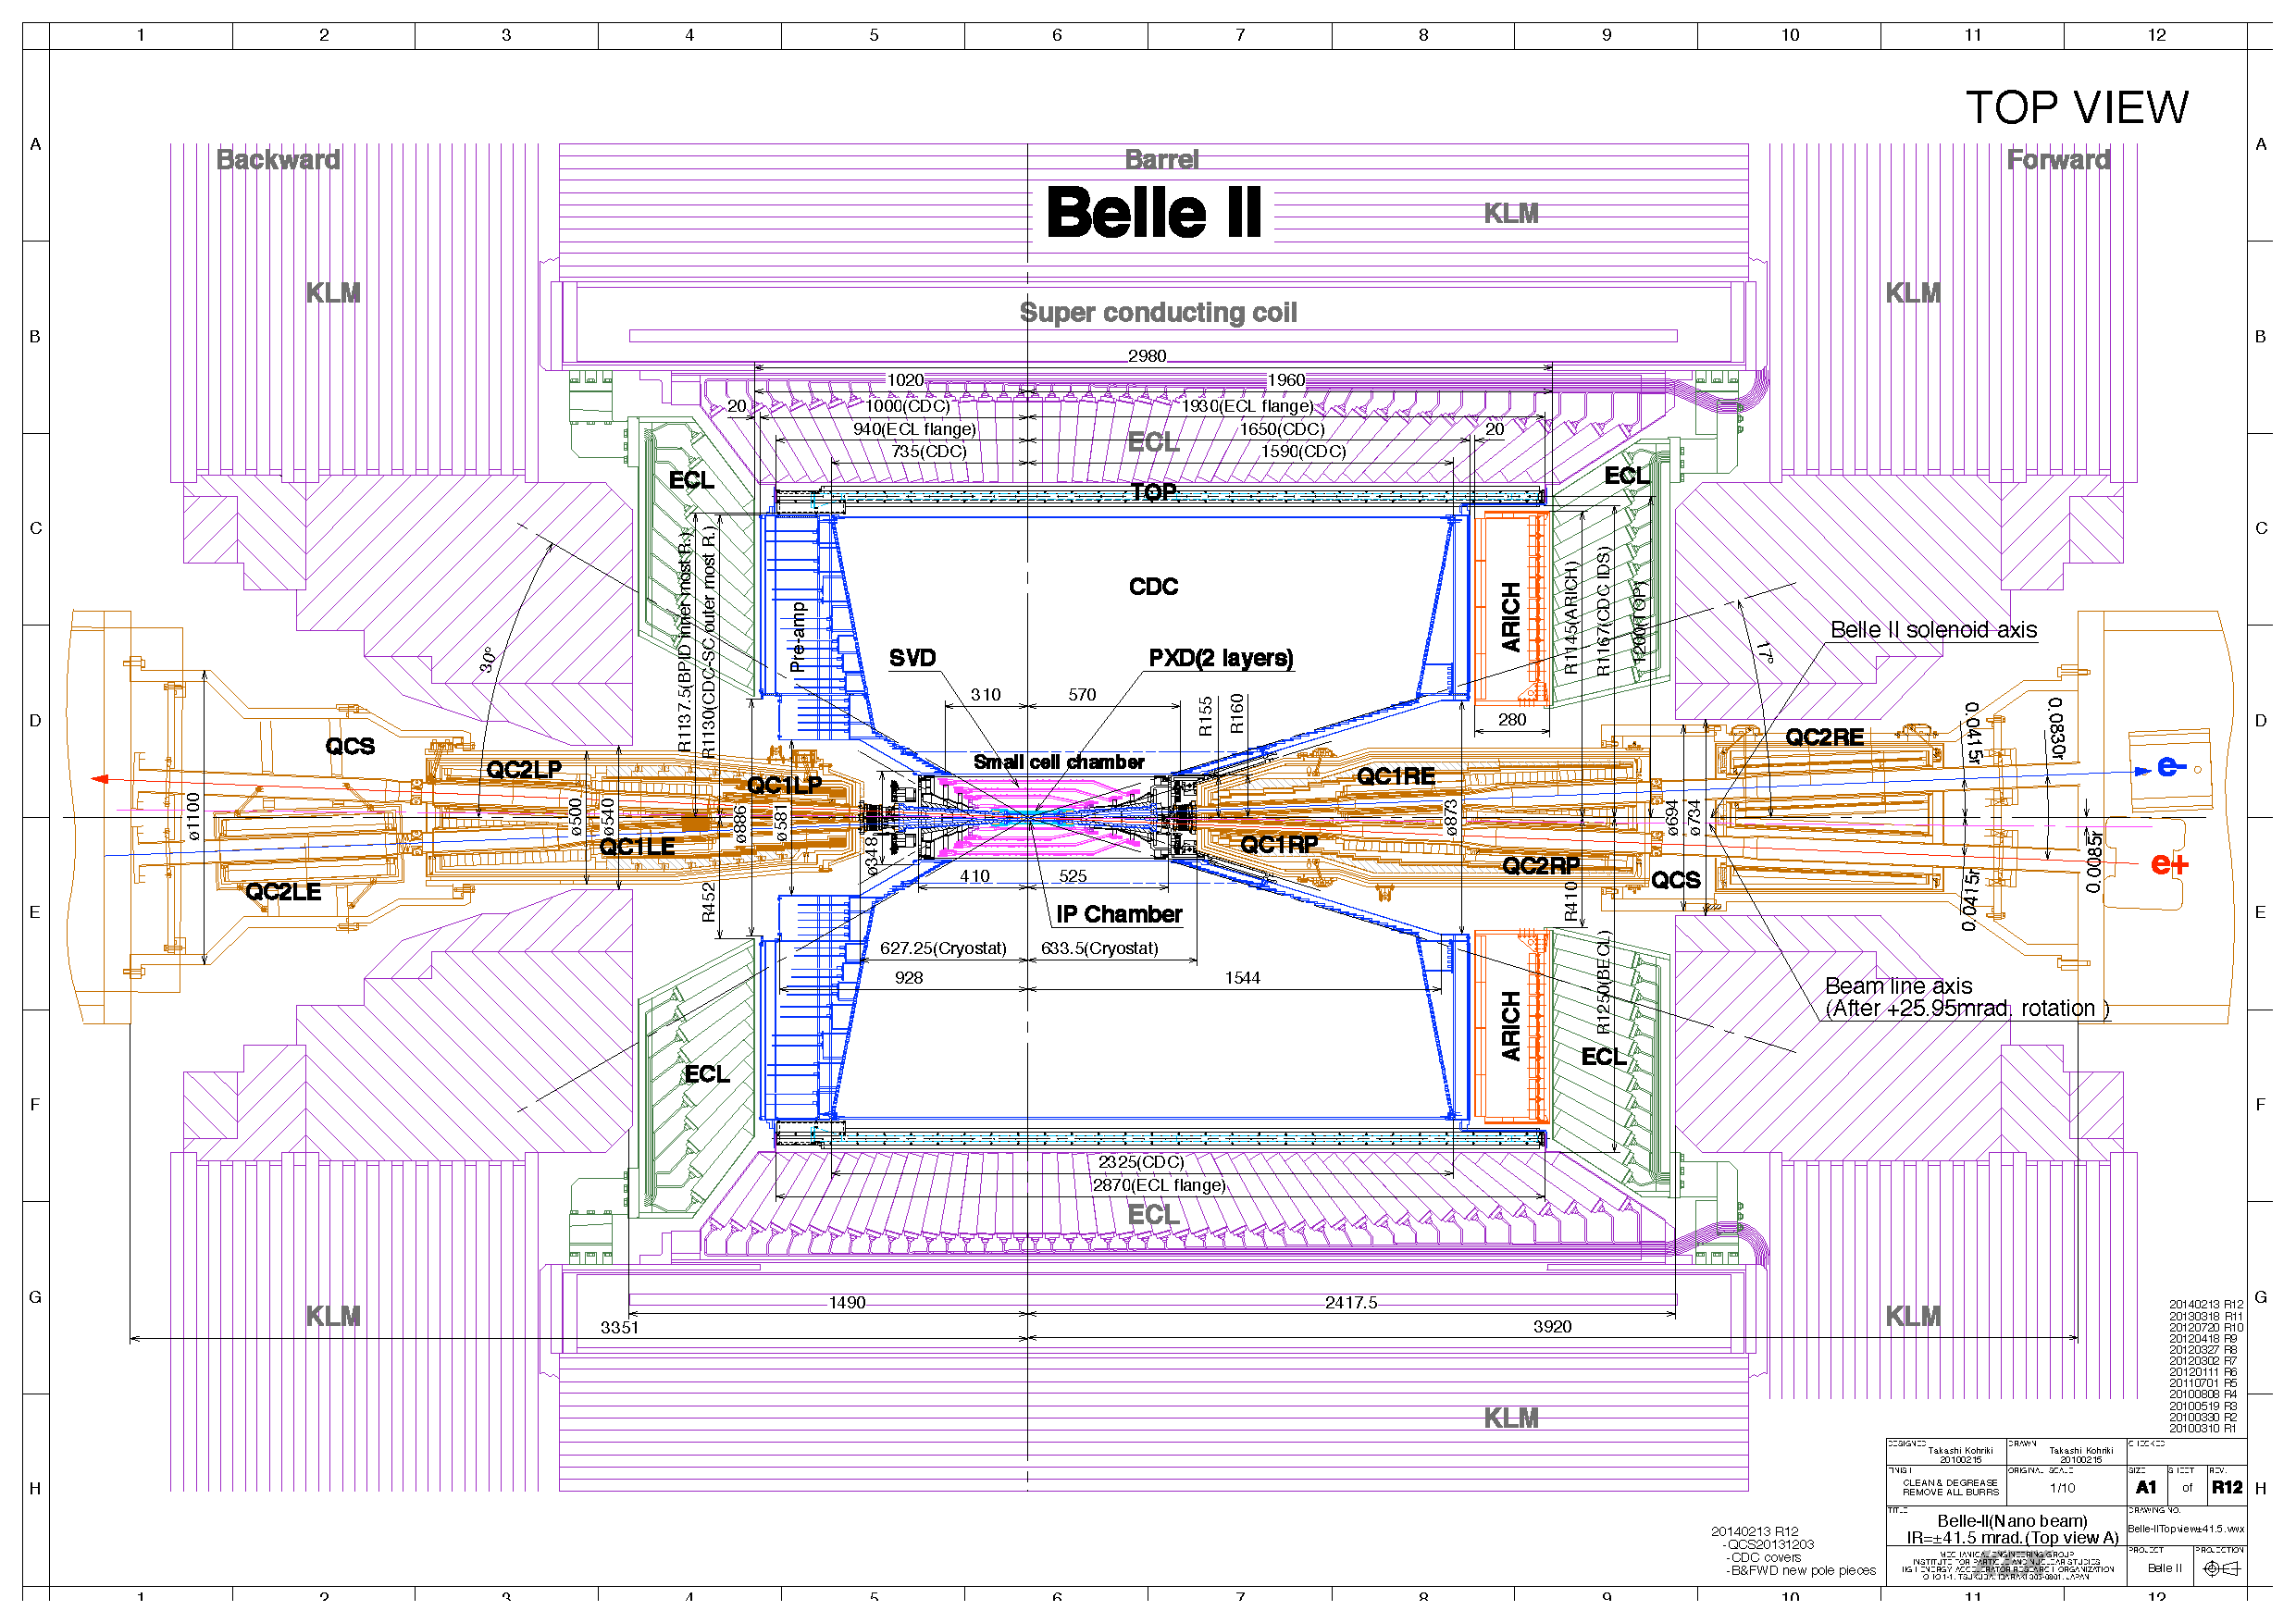
\includegraphics[width=0.7\textwidth]{BellellTopview}
        \end{centering}
    \end{figure}
\end{frame}
\begin{frame}
    \frametitle{Аэрогельная плитка}
    \begin{figure}
        \begin{centering}
            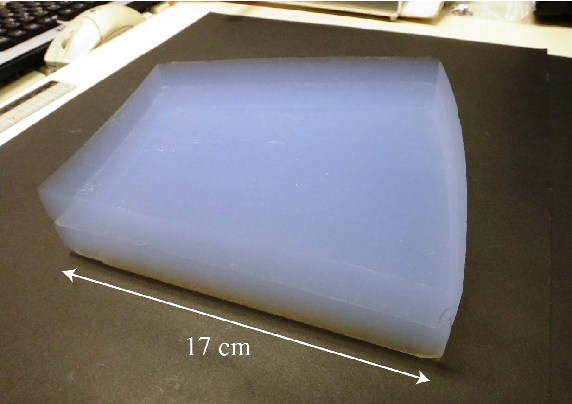
\includegraphics[width=0.7\textwidth]{aerogel-tile}
        \end{centering}
    \end{figure}
\end{frame}
\begin{frame}
    \frametitle{Аэрогель}
    \begin{figure}
        \begin{centering}
            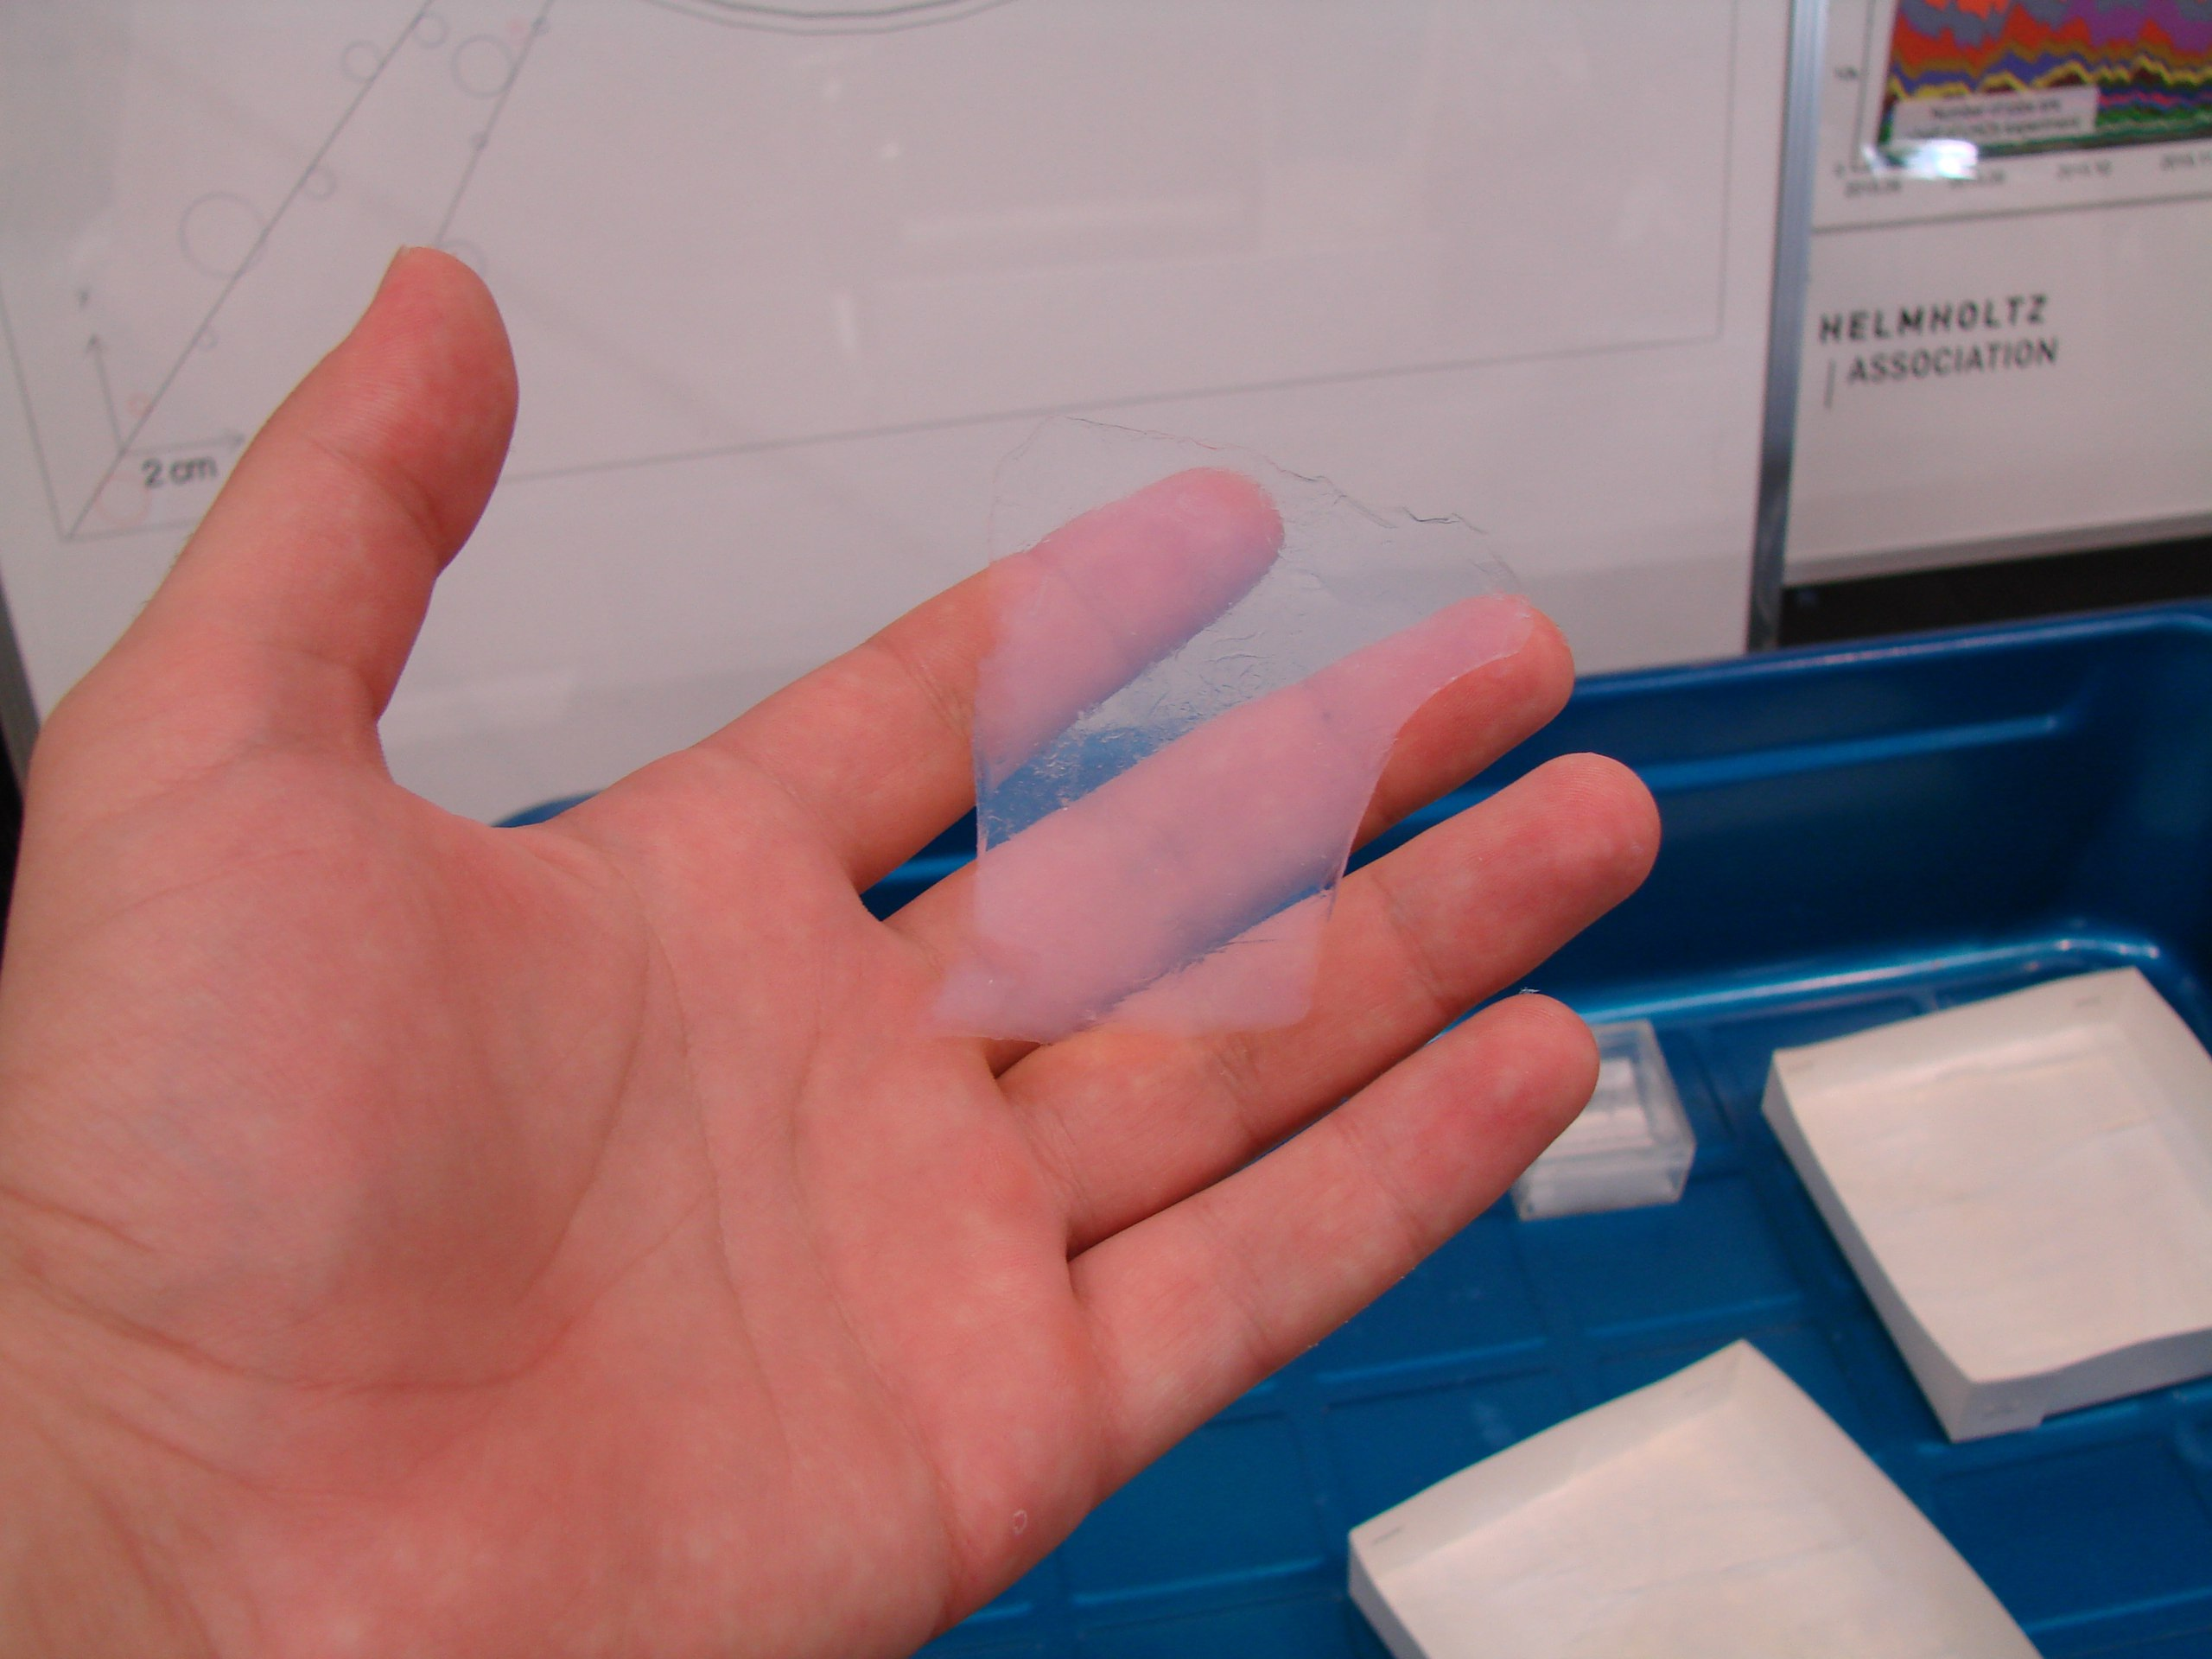
\includegraphics[width=0.7\textwidth]{aerogel}
        \end{centering}
    \end{figure}
\end{frame}
\begin{frame}
    \frametitle{Принцип детектора черенковских колец}
    \begin{figure}
        \begin{centering}
            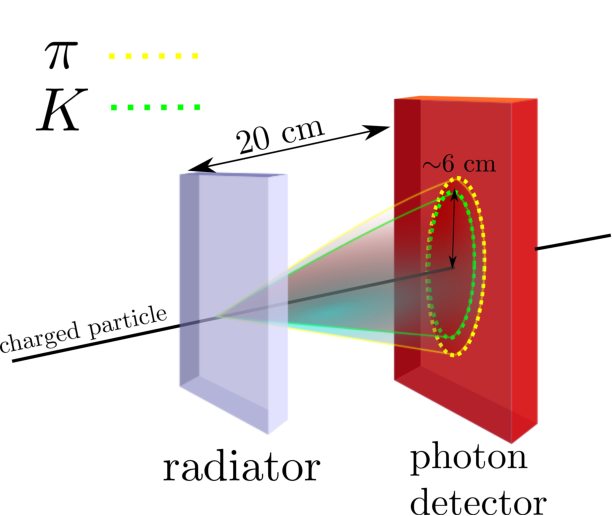
\includegraphics[width=0.7\textwidth]{arich-principle}
        \end{centering}
    \end{figure}
\end{frame}
\begin{frame}
    \frametitle{Аэрогелевый детектор черенковских колец}
    \begin{figure}
        \begin{centering}
            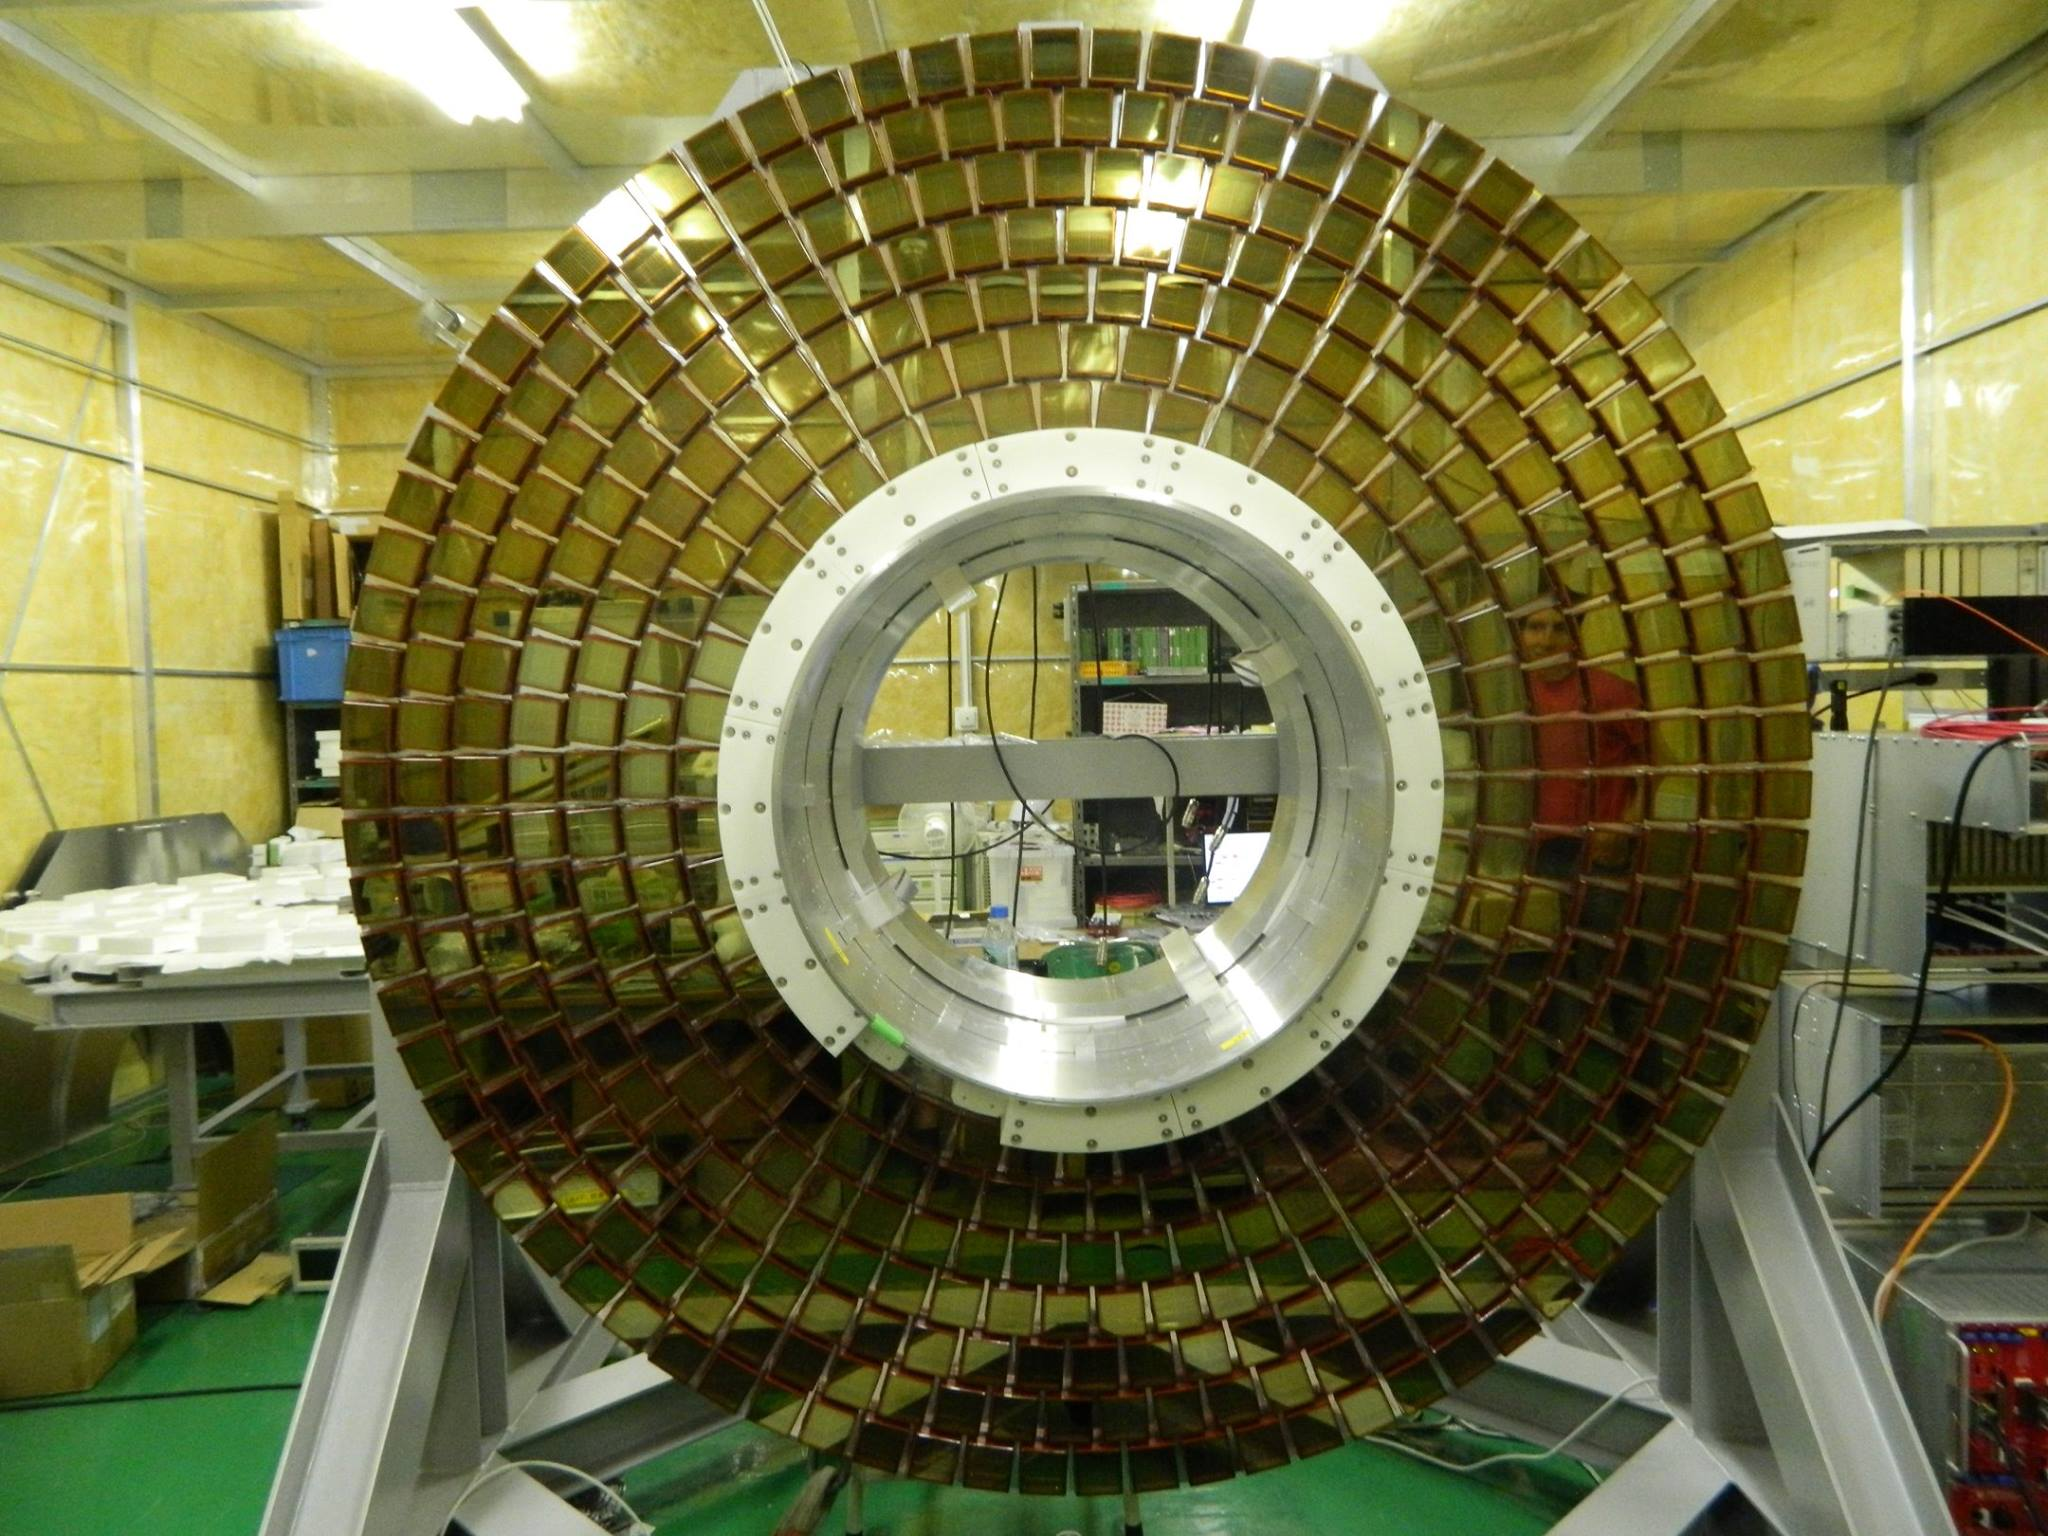
\includegraphics[width=0.7\textwidth]{belle-arich}
        \end{centering}
    \end{figure}
\end{frame}
\begin{frame}
    \frametitle{Симуляция прохождения заряженной частицы в ARICH}
    \begin{figure}
        \begin{centering}
            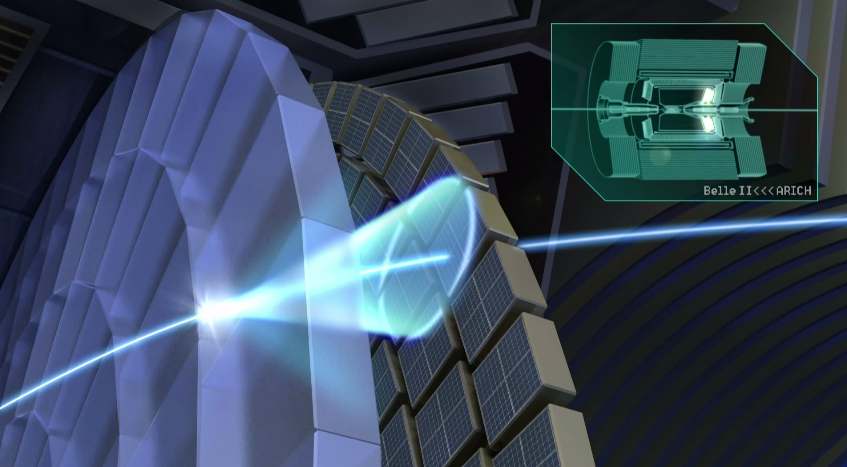
\includegraphics[width=0.7\textwidth]{arich-event}
        \end{centering}
    \end{figure}
\end{frame}
\begin{frame}
    \frametitle{Внутренний вид Belle II}
    \begin{figure}
        \begin{centering}
            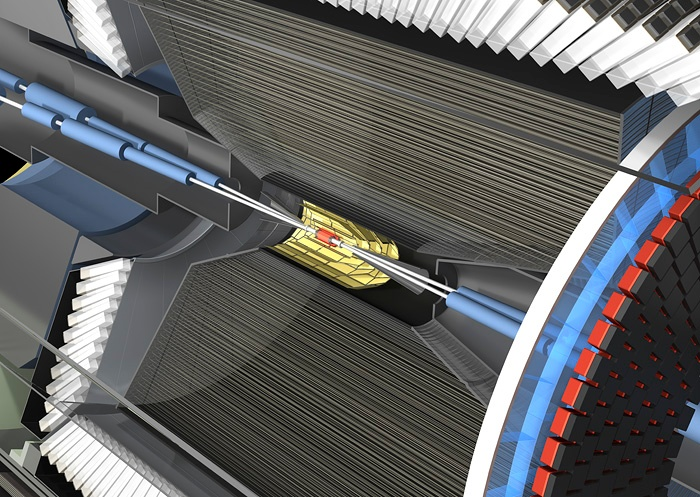
\includegraphics[width=0.7\textwidth]{belle2-inner}
        \end{centering}
    \end{figure}
\end{frame}
\begin{frame}
    \frametitle{Вершинный детектор}
    \begin{figure}
        \begin{centering}
            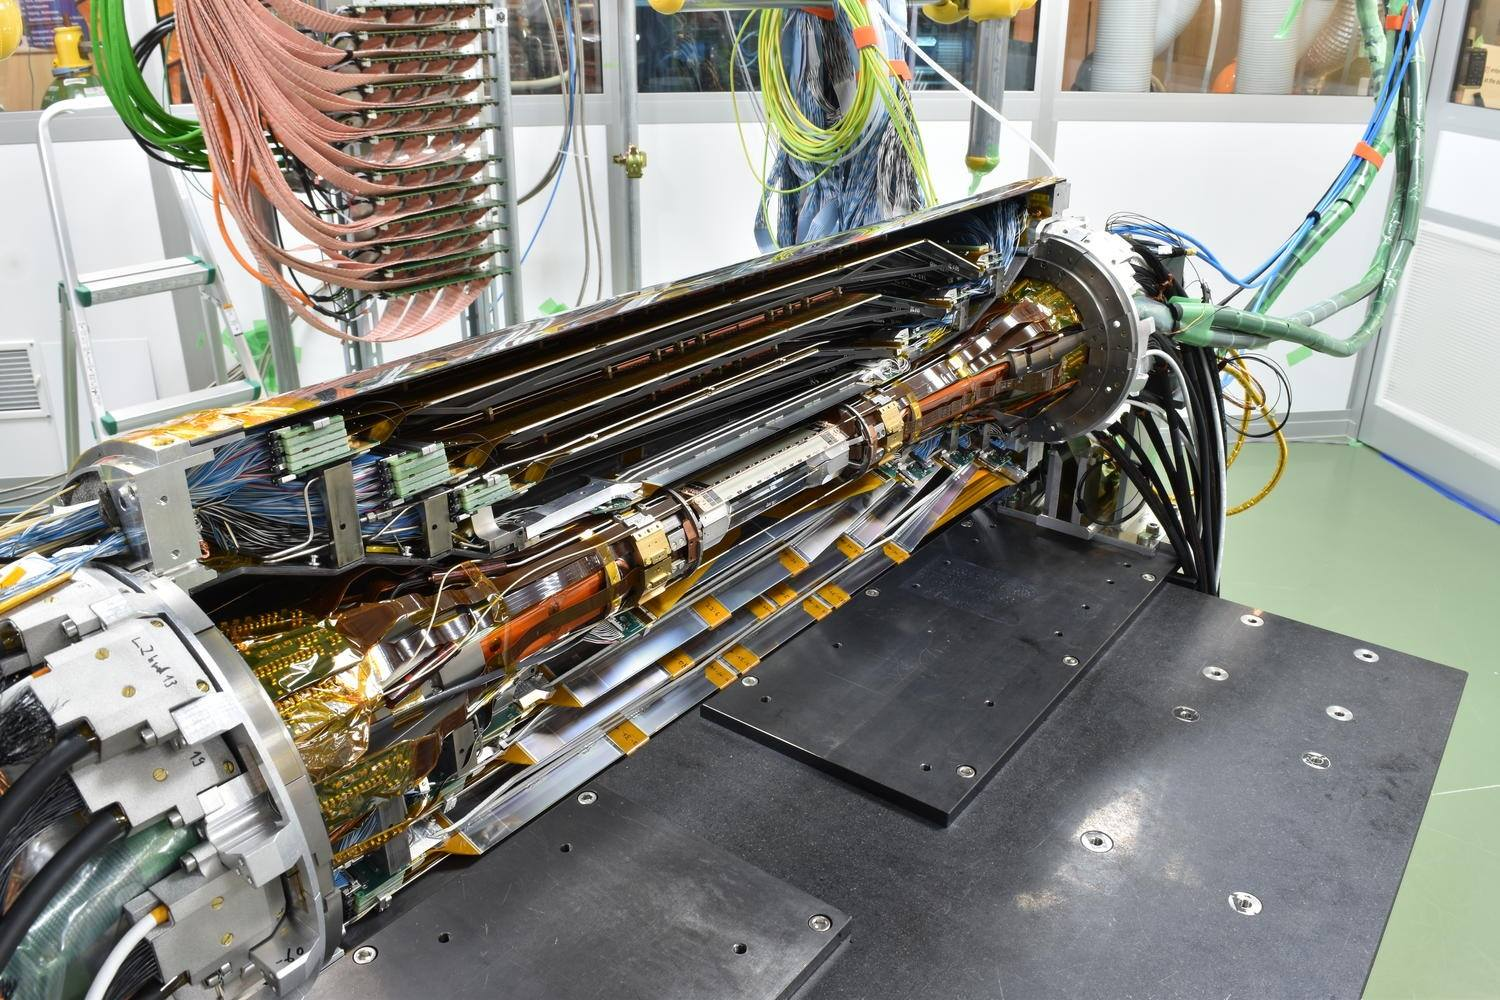
\includegraphics[width=0.7\textwidth]{belle-vxd}
        \end{centering}
    \end{figure}
\end{frame}
\begin{frame}
    \frametitle{Установка вершинного детектора в Belle II}
    \begin{figure}
        \begin{centering}
            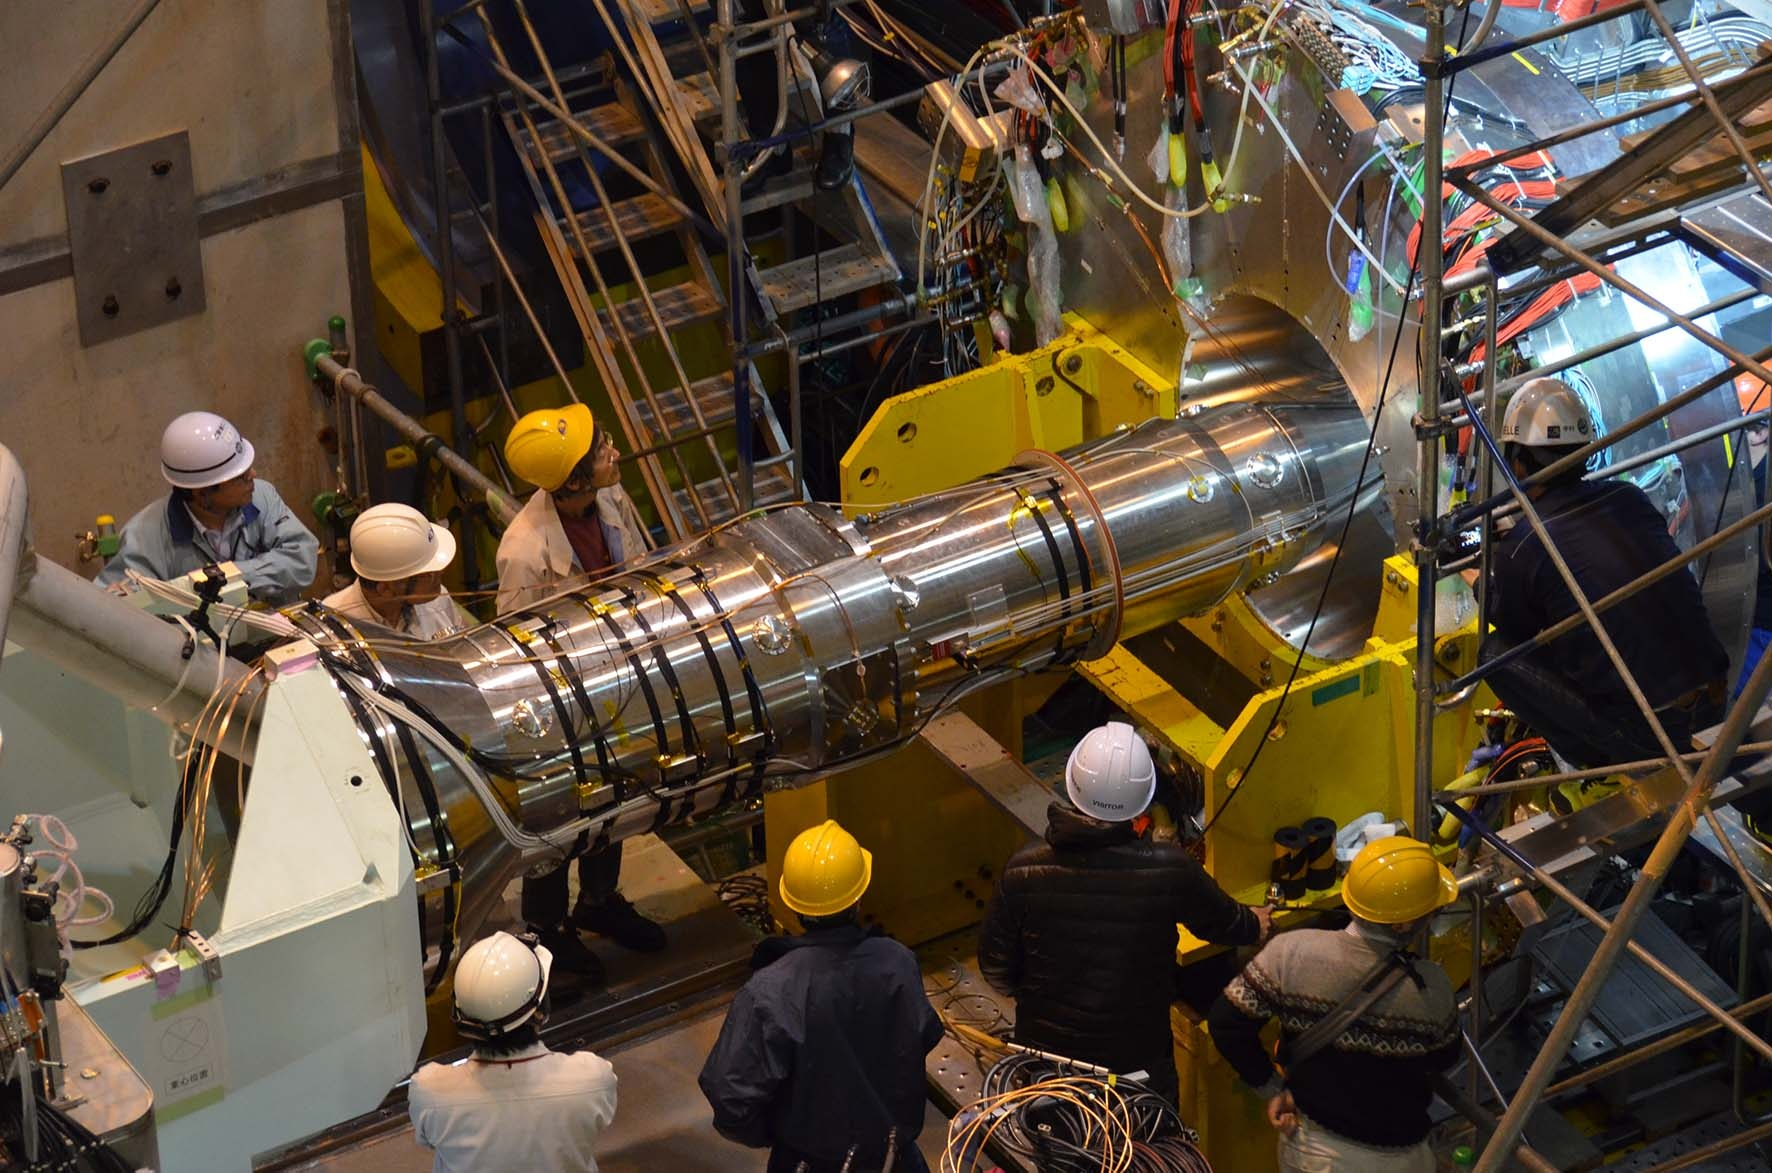
\includegraphics[width=0.7\textwidth]{belle-install}
        \end{centering}
    \end{figure}
\end{frame}
	
\begin{frame}
    \begin{figure}
        \begin{centering}
            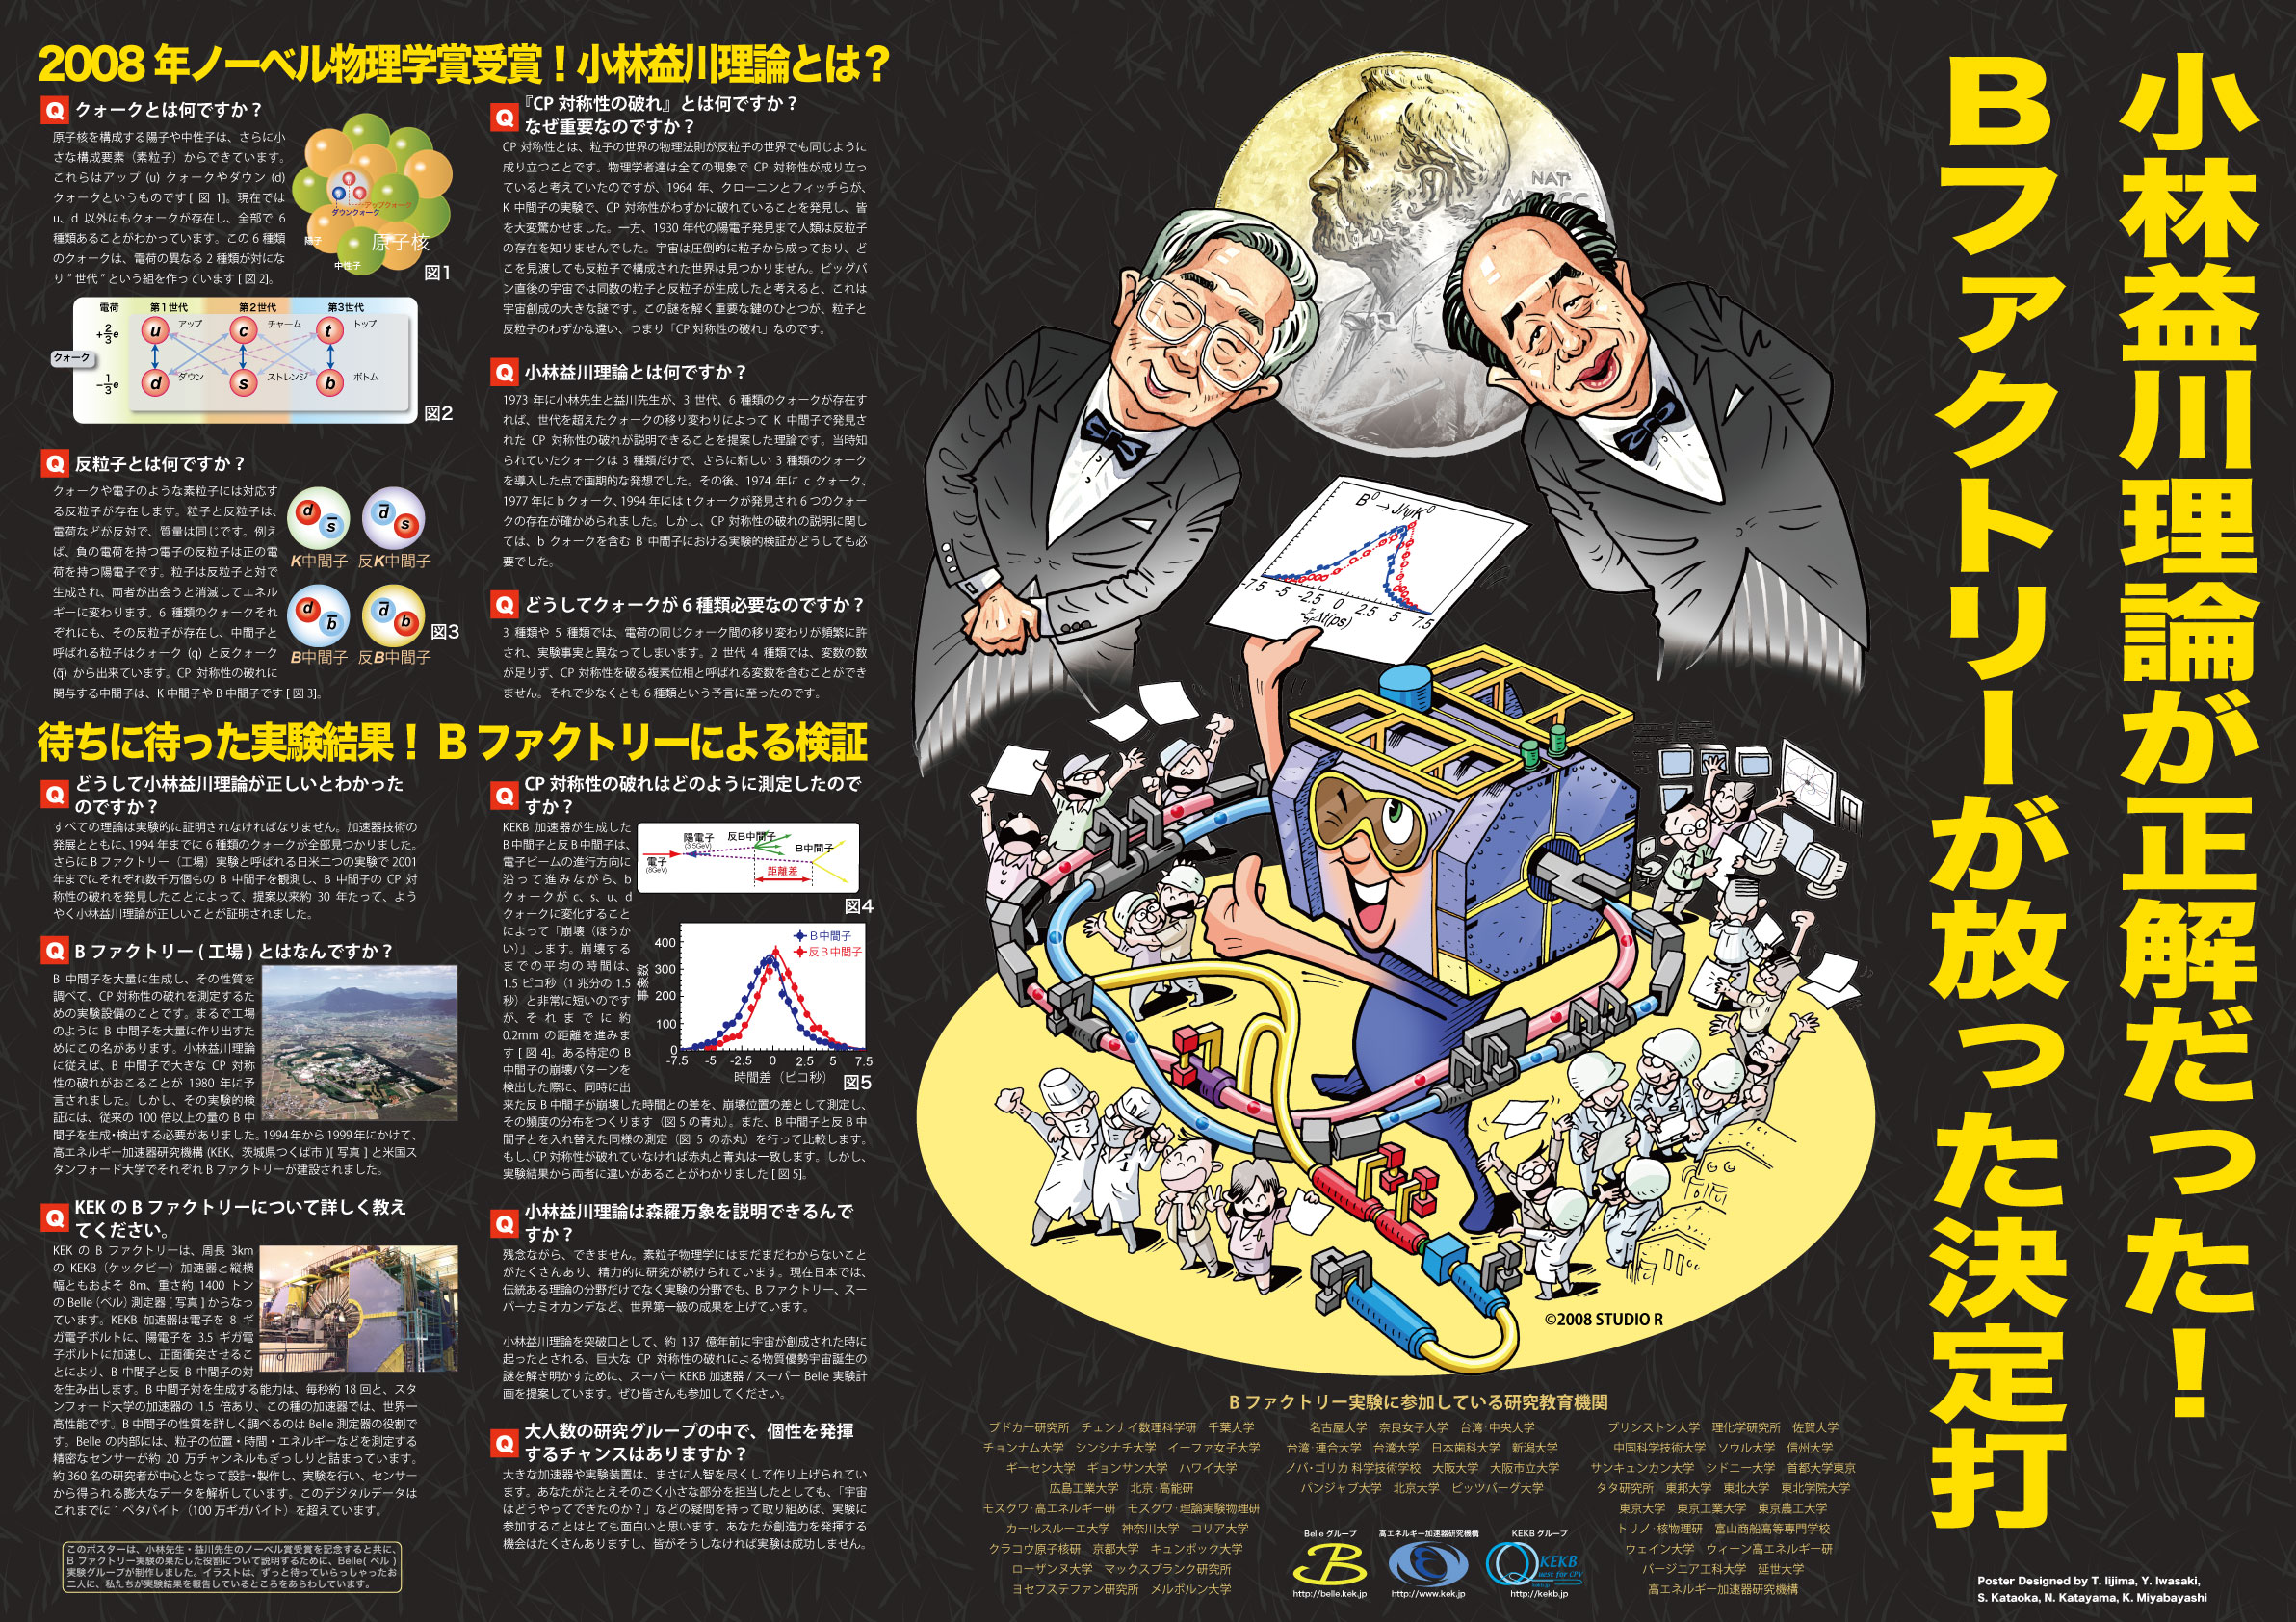
\includegraphics[width=0.95\textwidth]{KM-poster}
        \end{centering}
    \end{figure}
\end{frame}

\subsection{LHC}
\begin{frame}
    {\LARGE Большой адронный коллайдер}
\end{frame}
\begin{frame}
    \frametitle{Большой адронный коллайдер где-то рядом}
    \begin{figure}
        \begin{centering}
            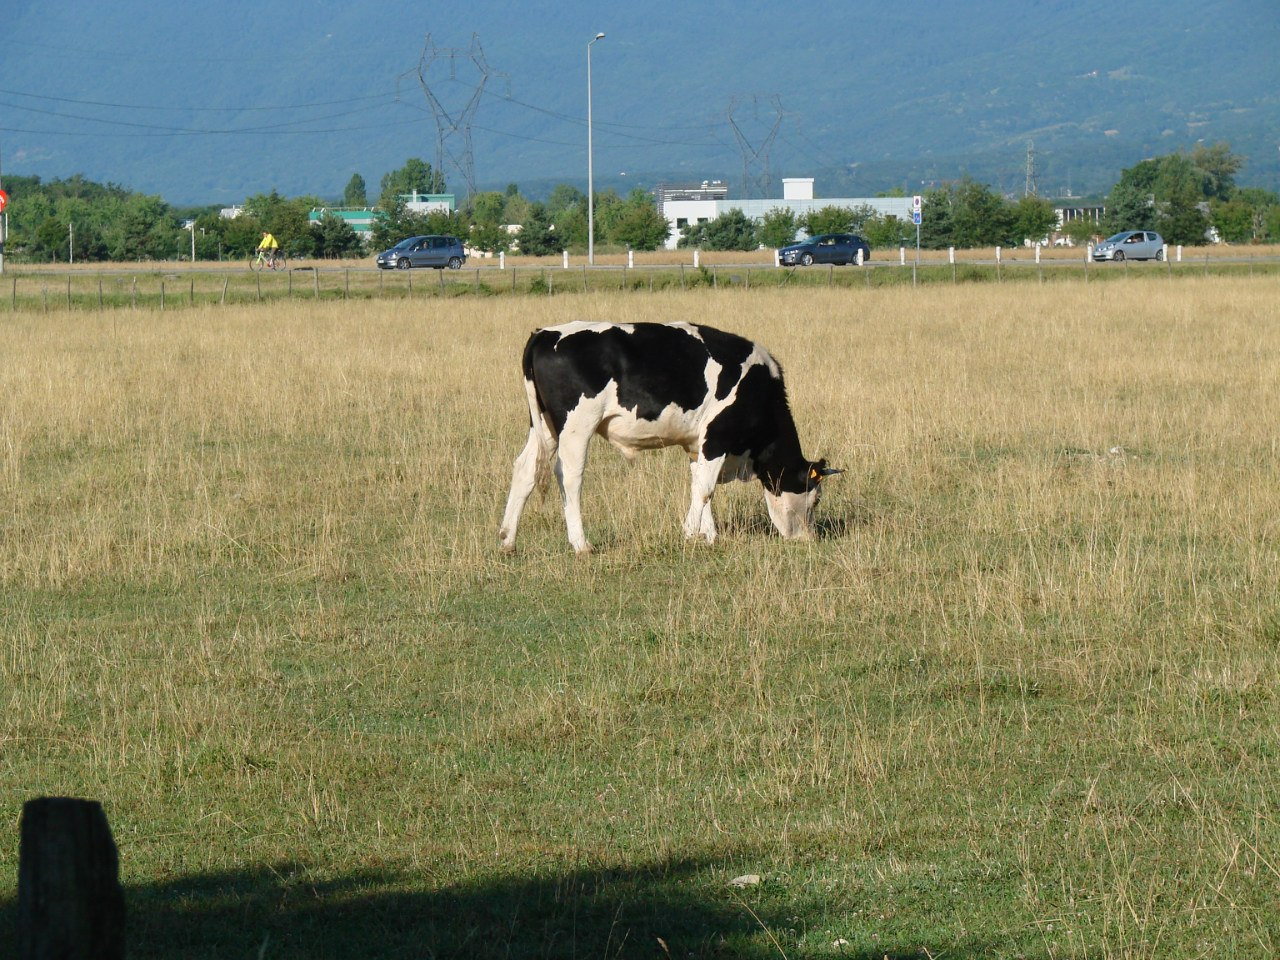
\includegraphics[width=0.7\textwidth]{lhc-top}
        \end{centering}
    \end{figure}
\end{frame}
\begin{frame}
    \begin{figure}
        \begin{centering}
            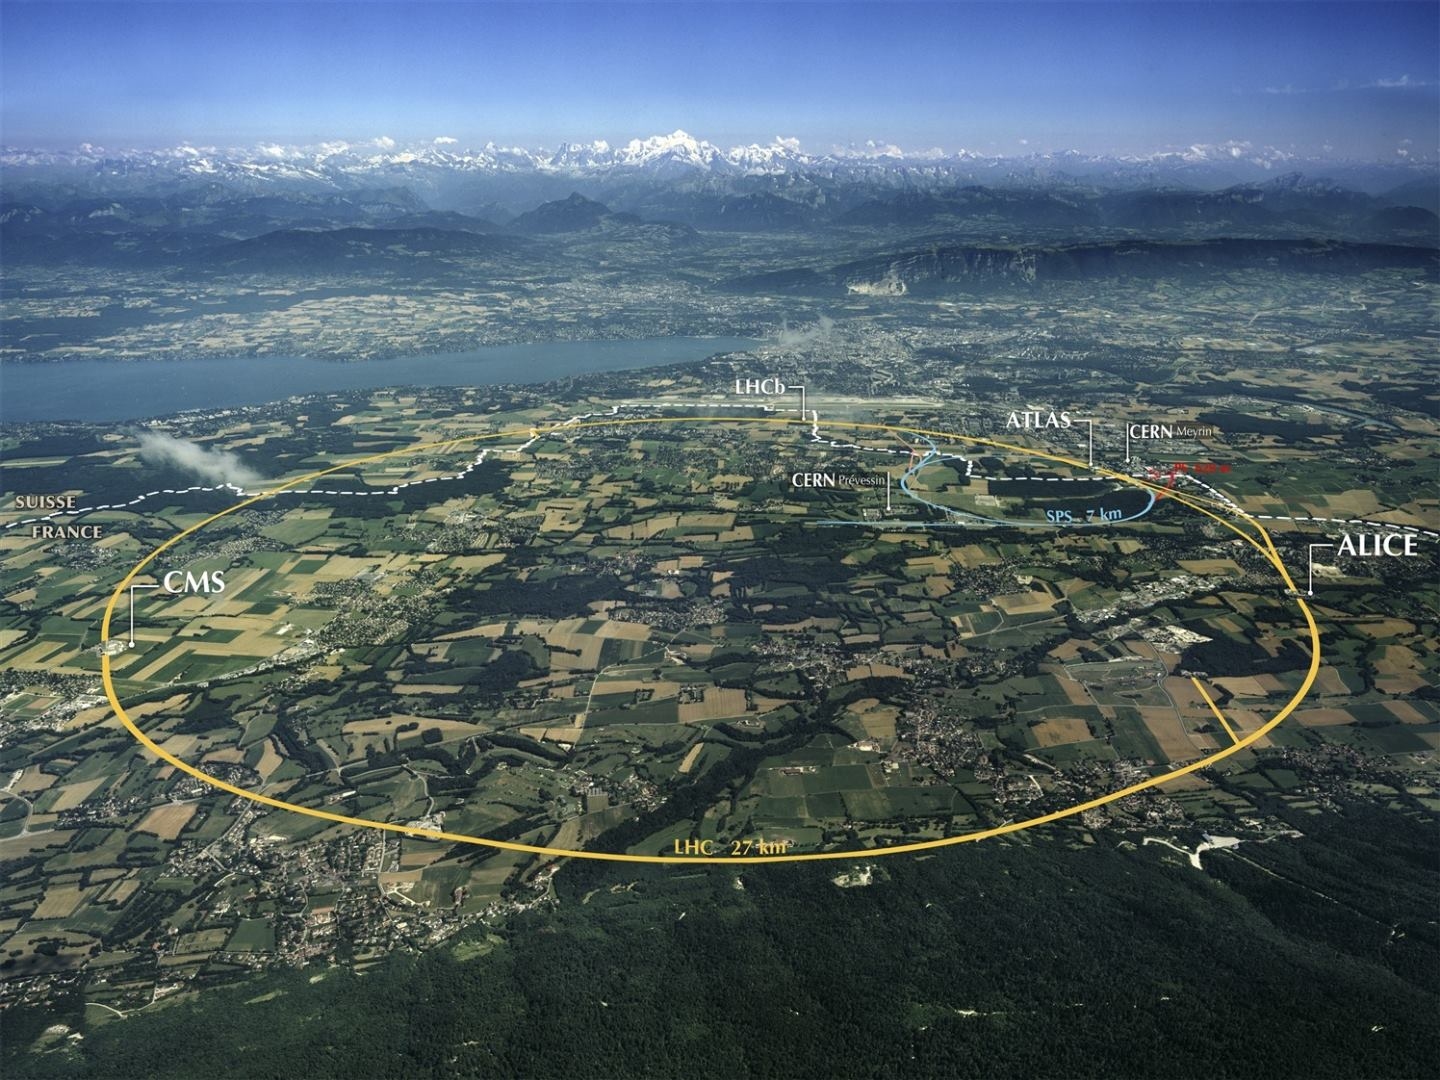
\includegraphics[width=0.7\textwidth]{lhc}
        \end{centering}
    \end{figure}
\end{frame}
\begin{frame}
    \begin{figure}
        \begin{centering}
            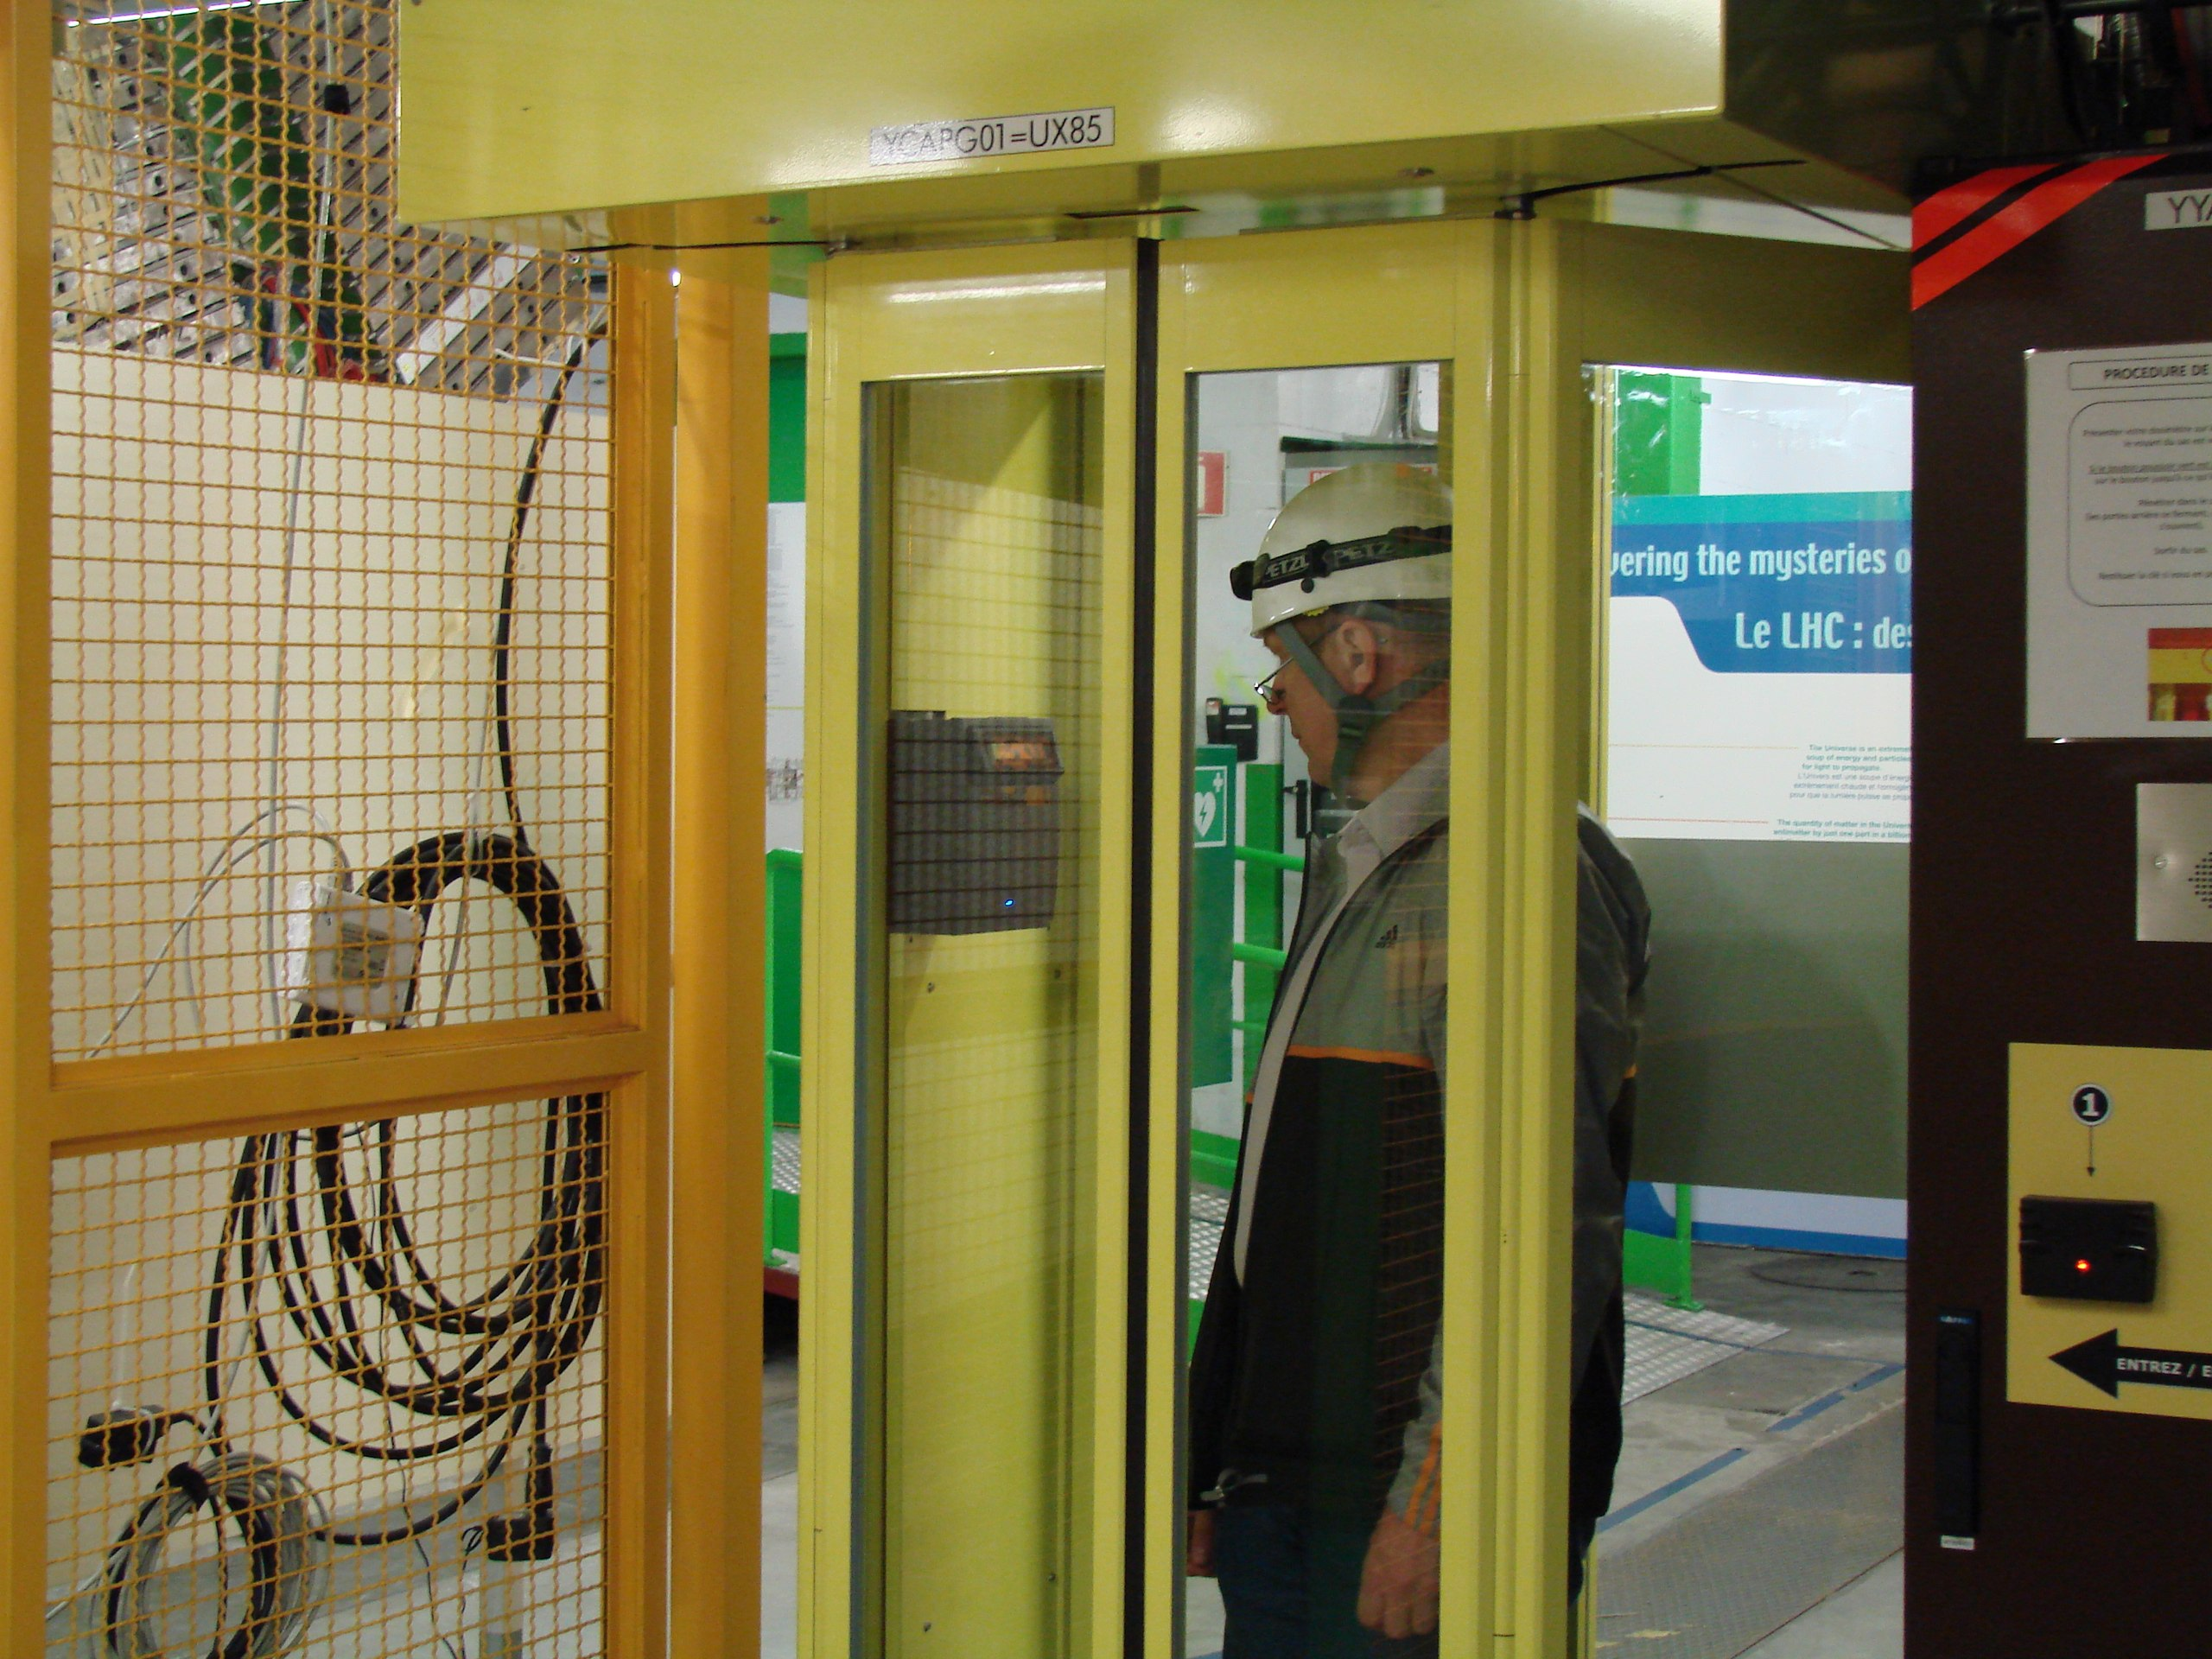
\includegraphics[width=0.7\textwidth]{eye-scan}
        \end{centering}
    \end{figure}
\end{frame}
\begin{frame}
    \frametitle{Транспорт для коллайдера}
    \begin{figure}
        \begin{centering}
            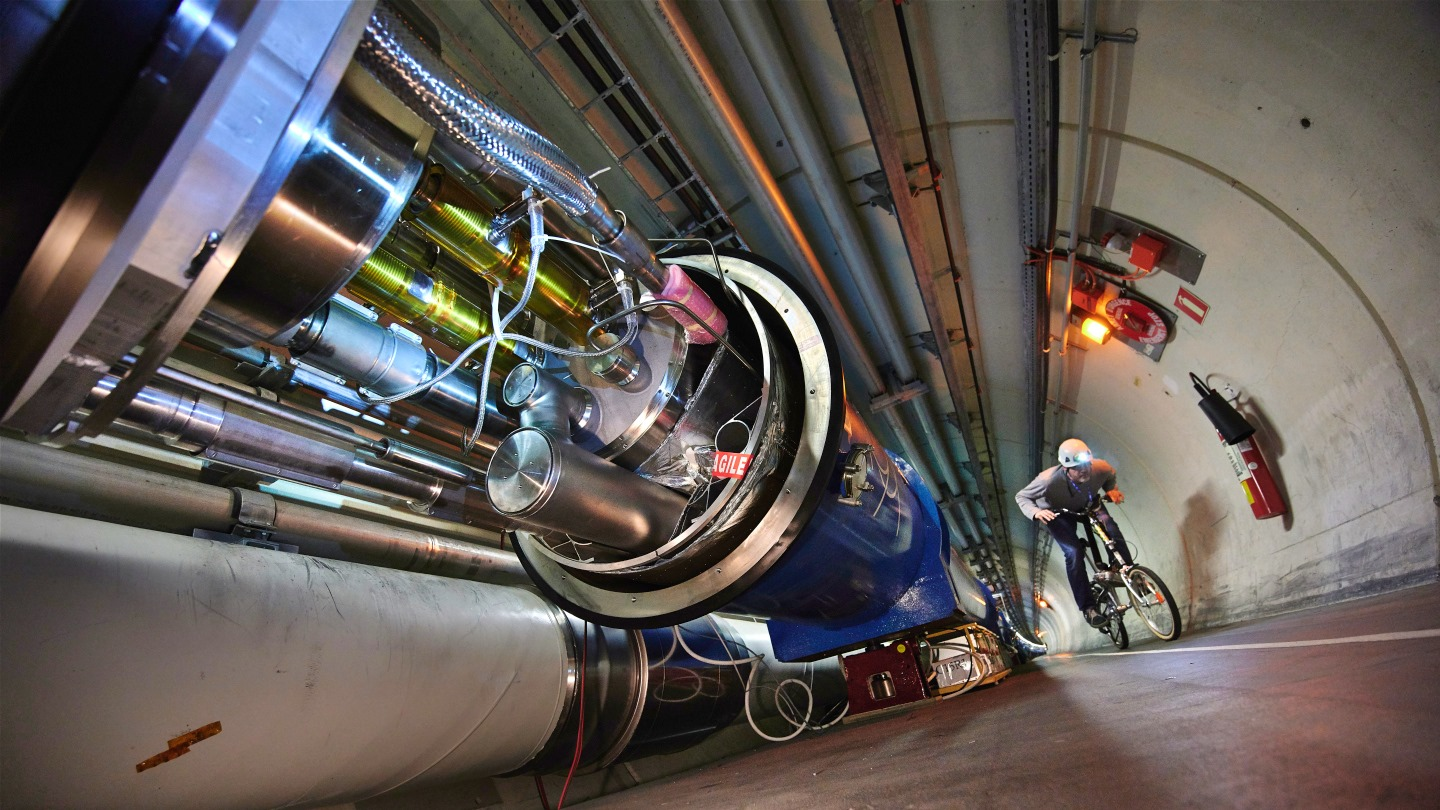
\includegraphics[width=0.85\textwidth]{lhc-bike}
        \end{centering}
    \end{figure}
\end{frame}
\begin{frame}
    \begin{figure}
        \begin{centering}
            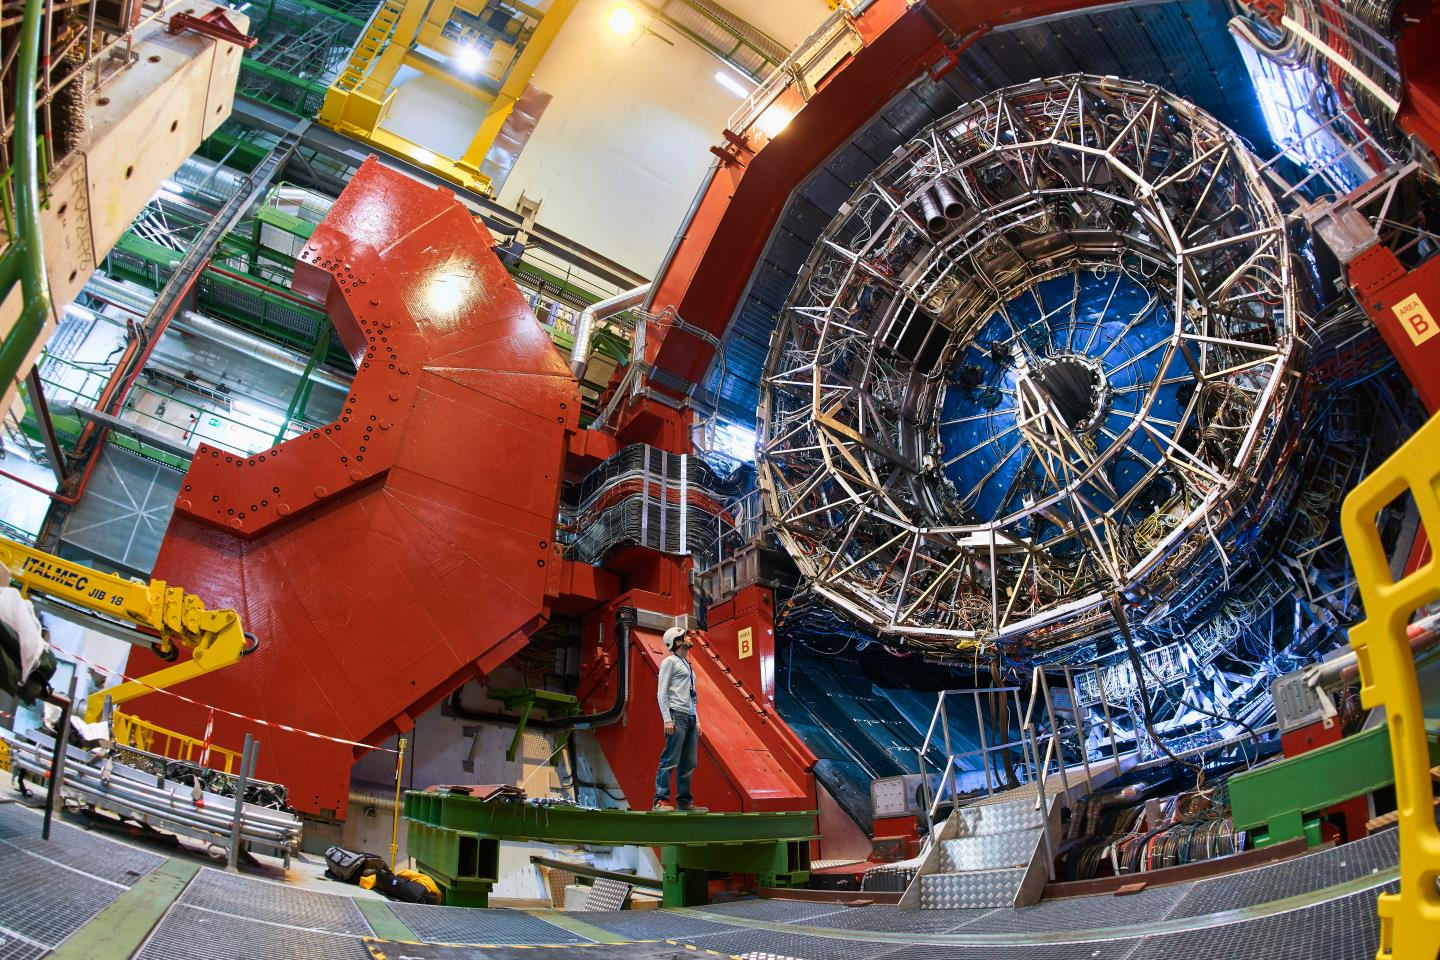
\includegraphics[width=0.8\textwidth]{alice}
        \end{centering}
    \end{figure}
\end{frame}
\begin{frame}
    \begin{figure}
        \begin{centering}
            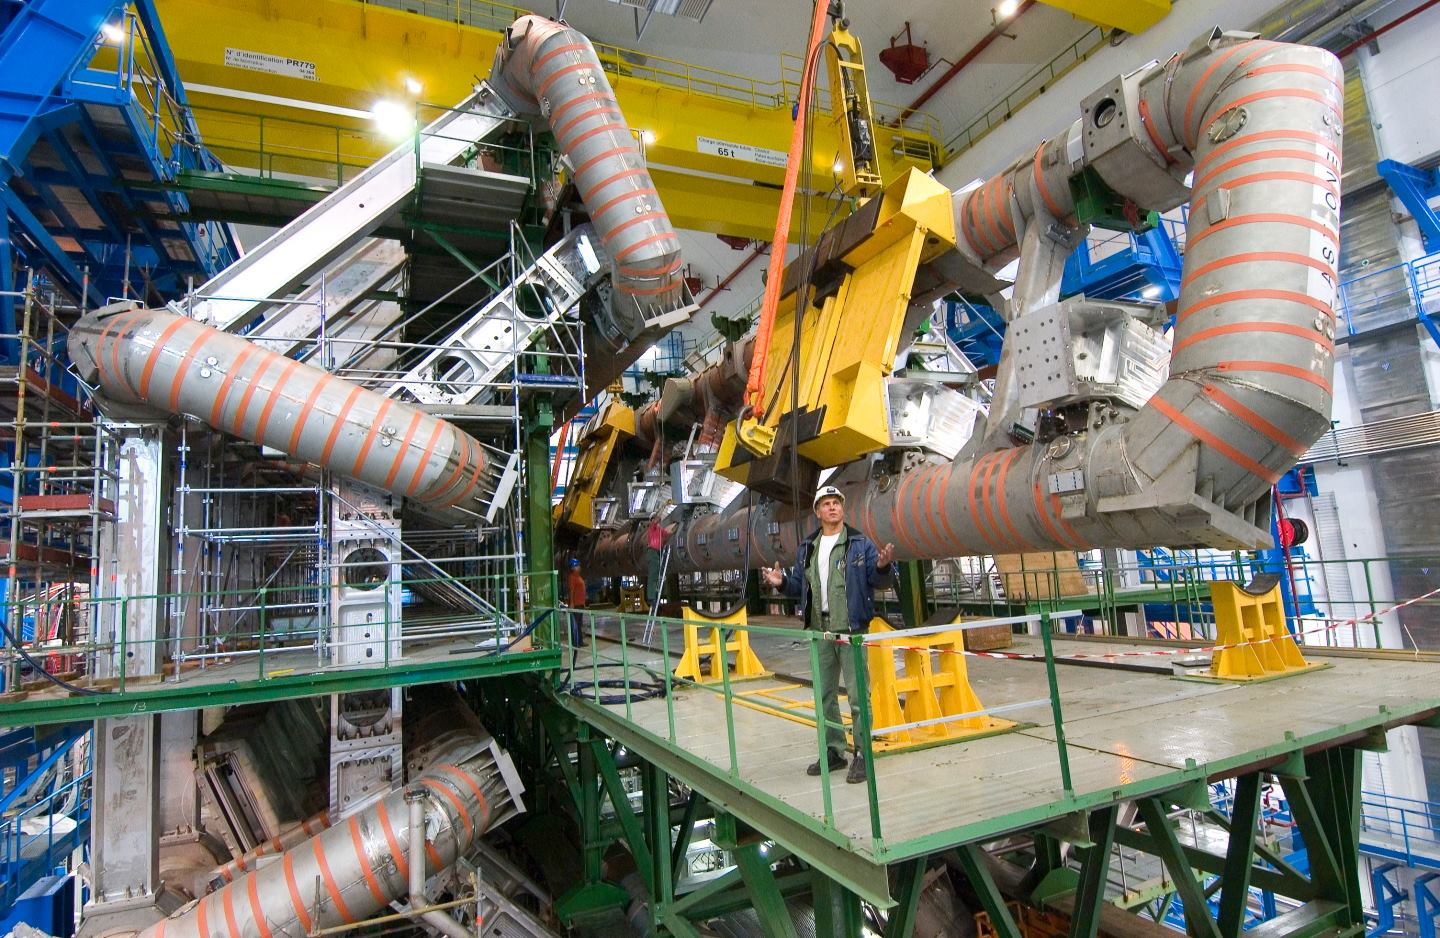
\includegraphics[width=0.8\textwidth]{atlas}
        \end{centering}
    \end{figure}
\end{frame}
\begin{frame}
    \begin{figure}
        \begin{centering}
            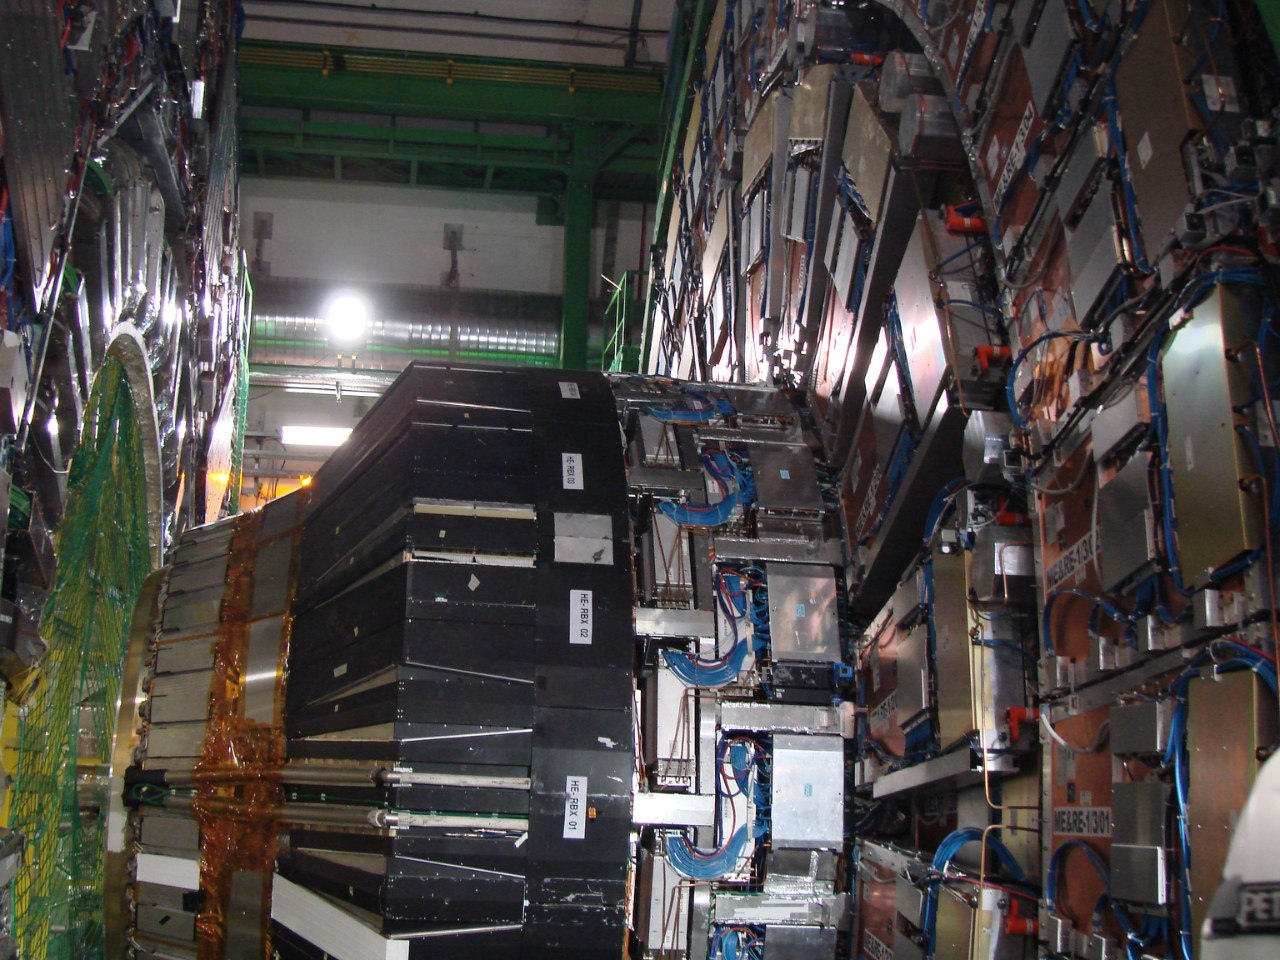
\includegraphics[width=0.8\textwidth]{cms}
        \end{centering}
    \end{figure}
\end{frame}
\begin{frame}
    \begin{figure}
        \begin{centering}
            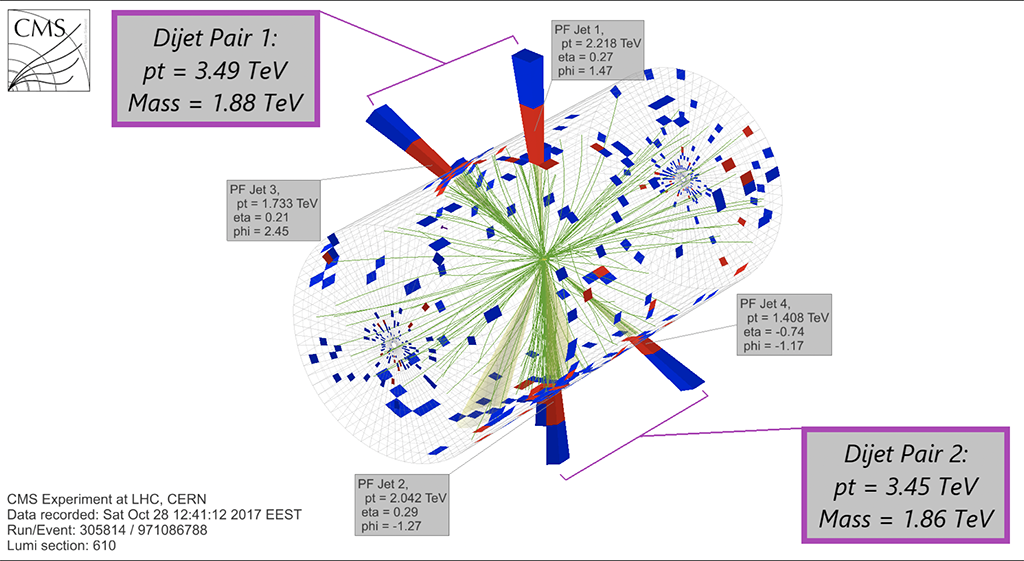
\includegraphics[width=0.9\textwidth]{cms-ed}
        \end{centering}
    \end{figure}
\end{frame}
\begin{frame}
    \begin{figure}
        \begin{centering}
            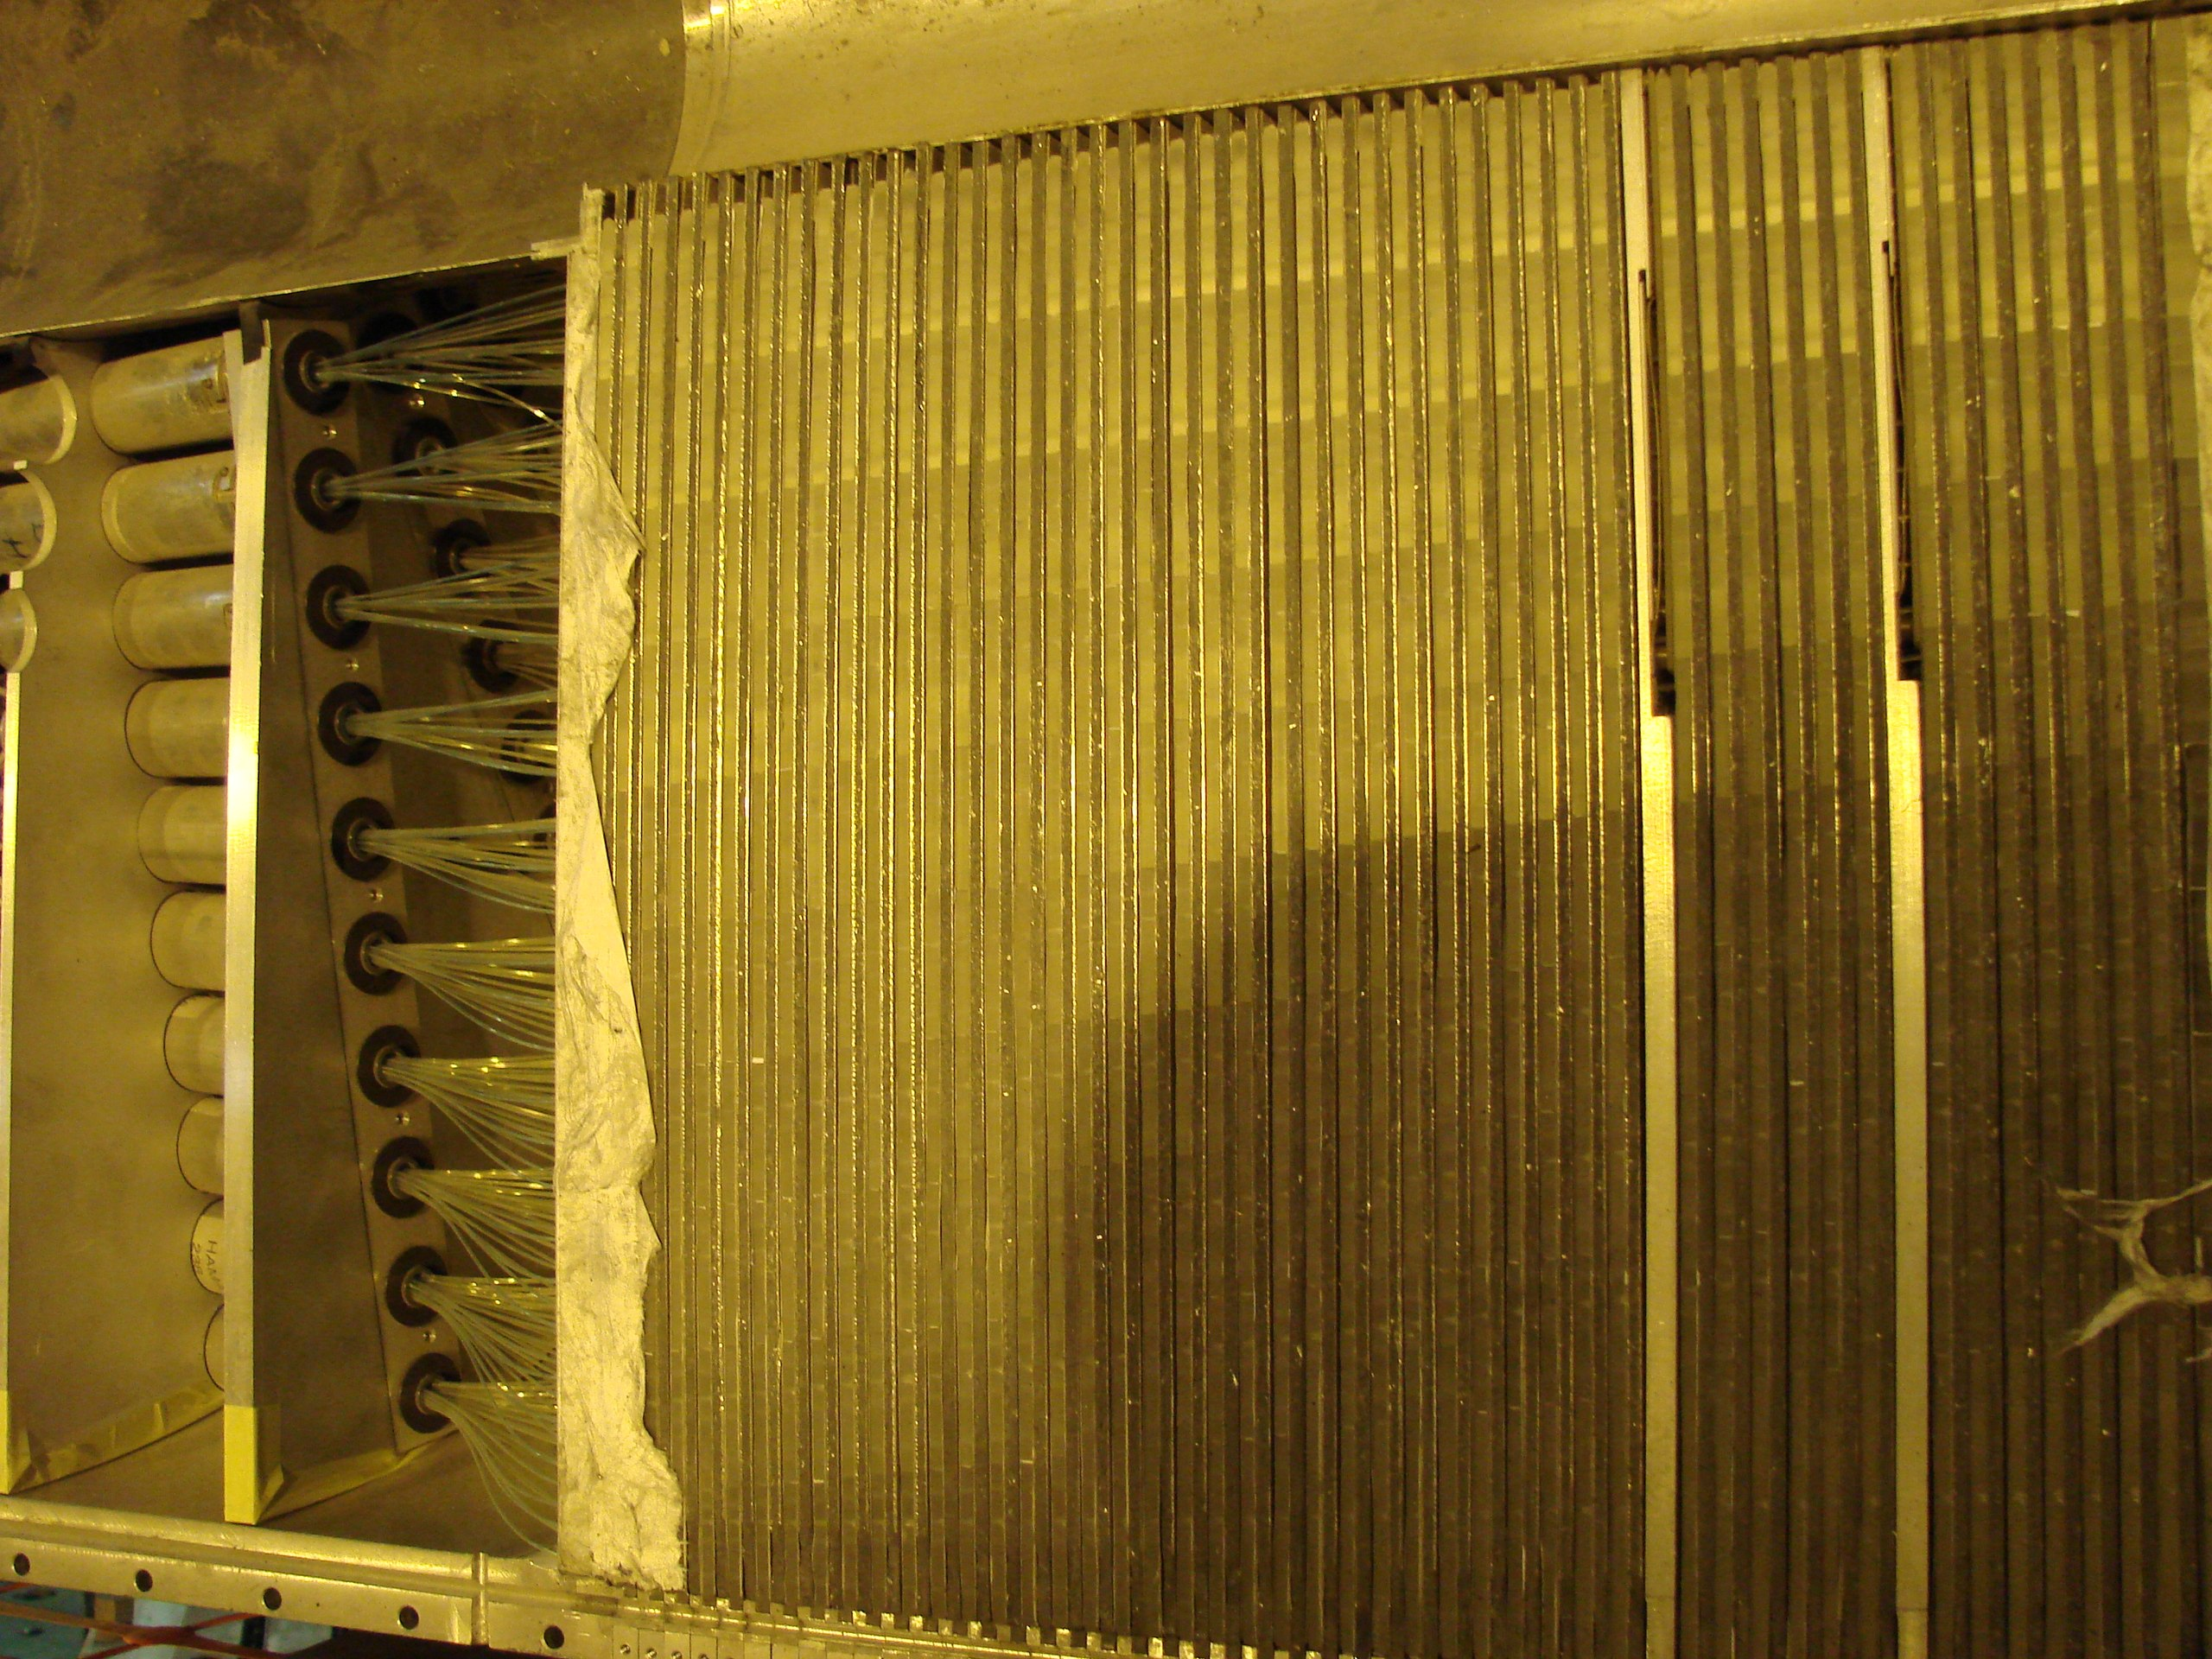
\includegraphics[width=0.7\textwidth]{hcal}
        \end{centering}
    \end{figure}
\end{frame}
\begin{frame}
    \begin{figure}
        \begin{centering}
            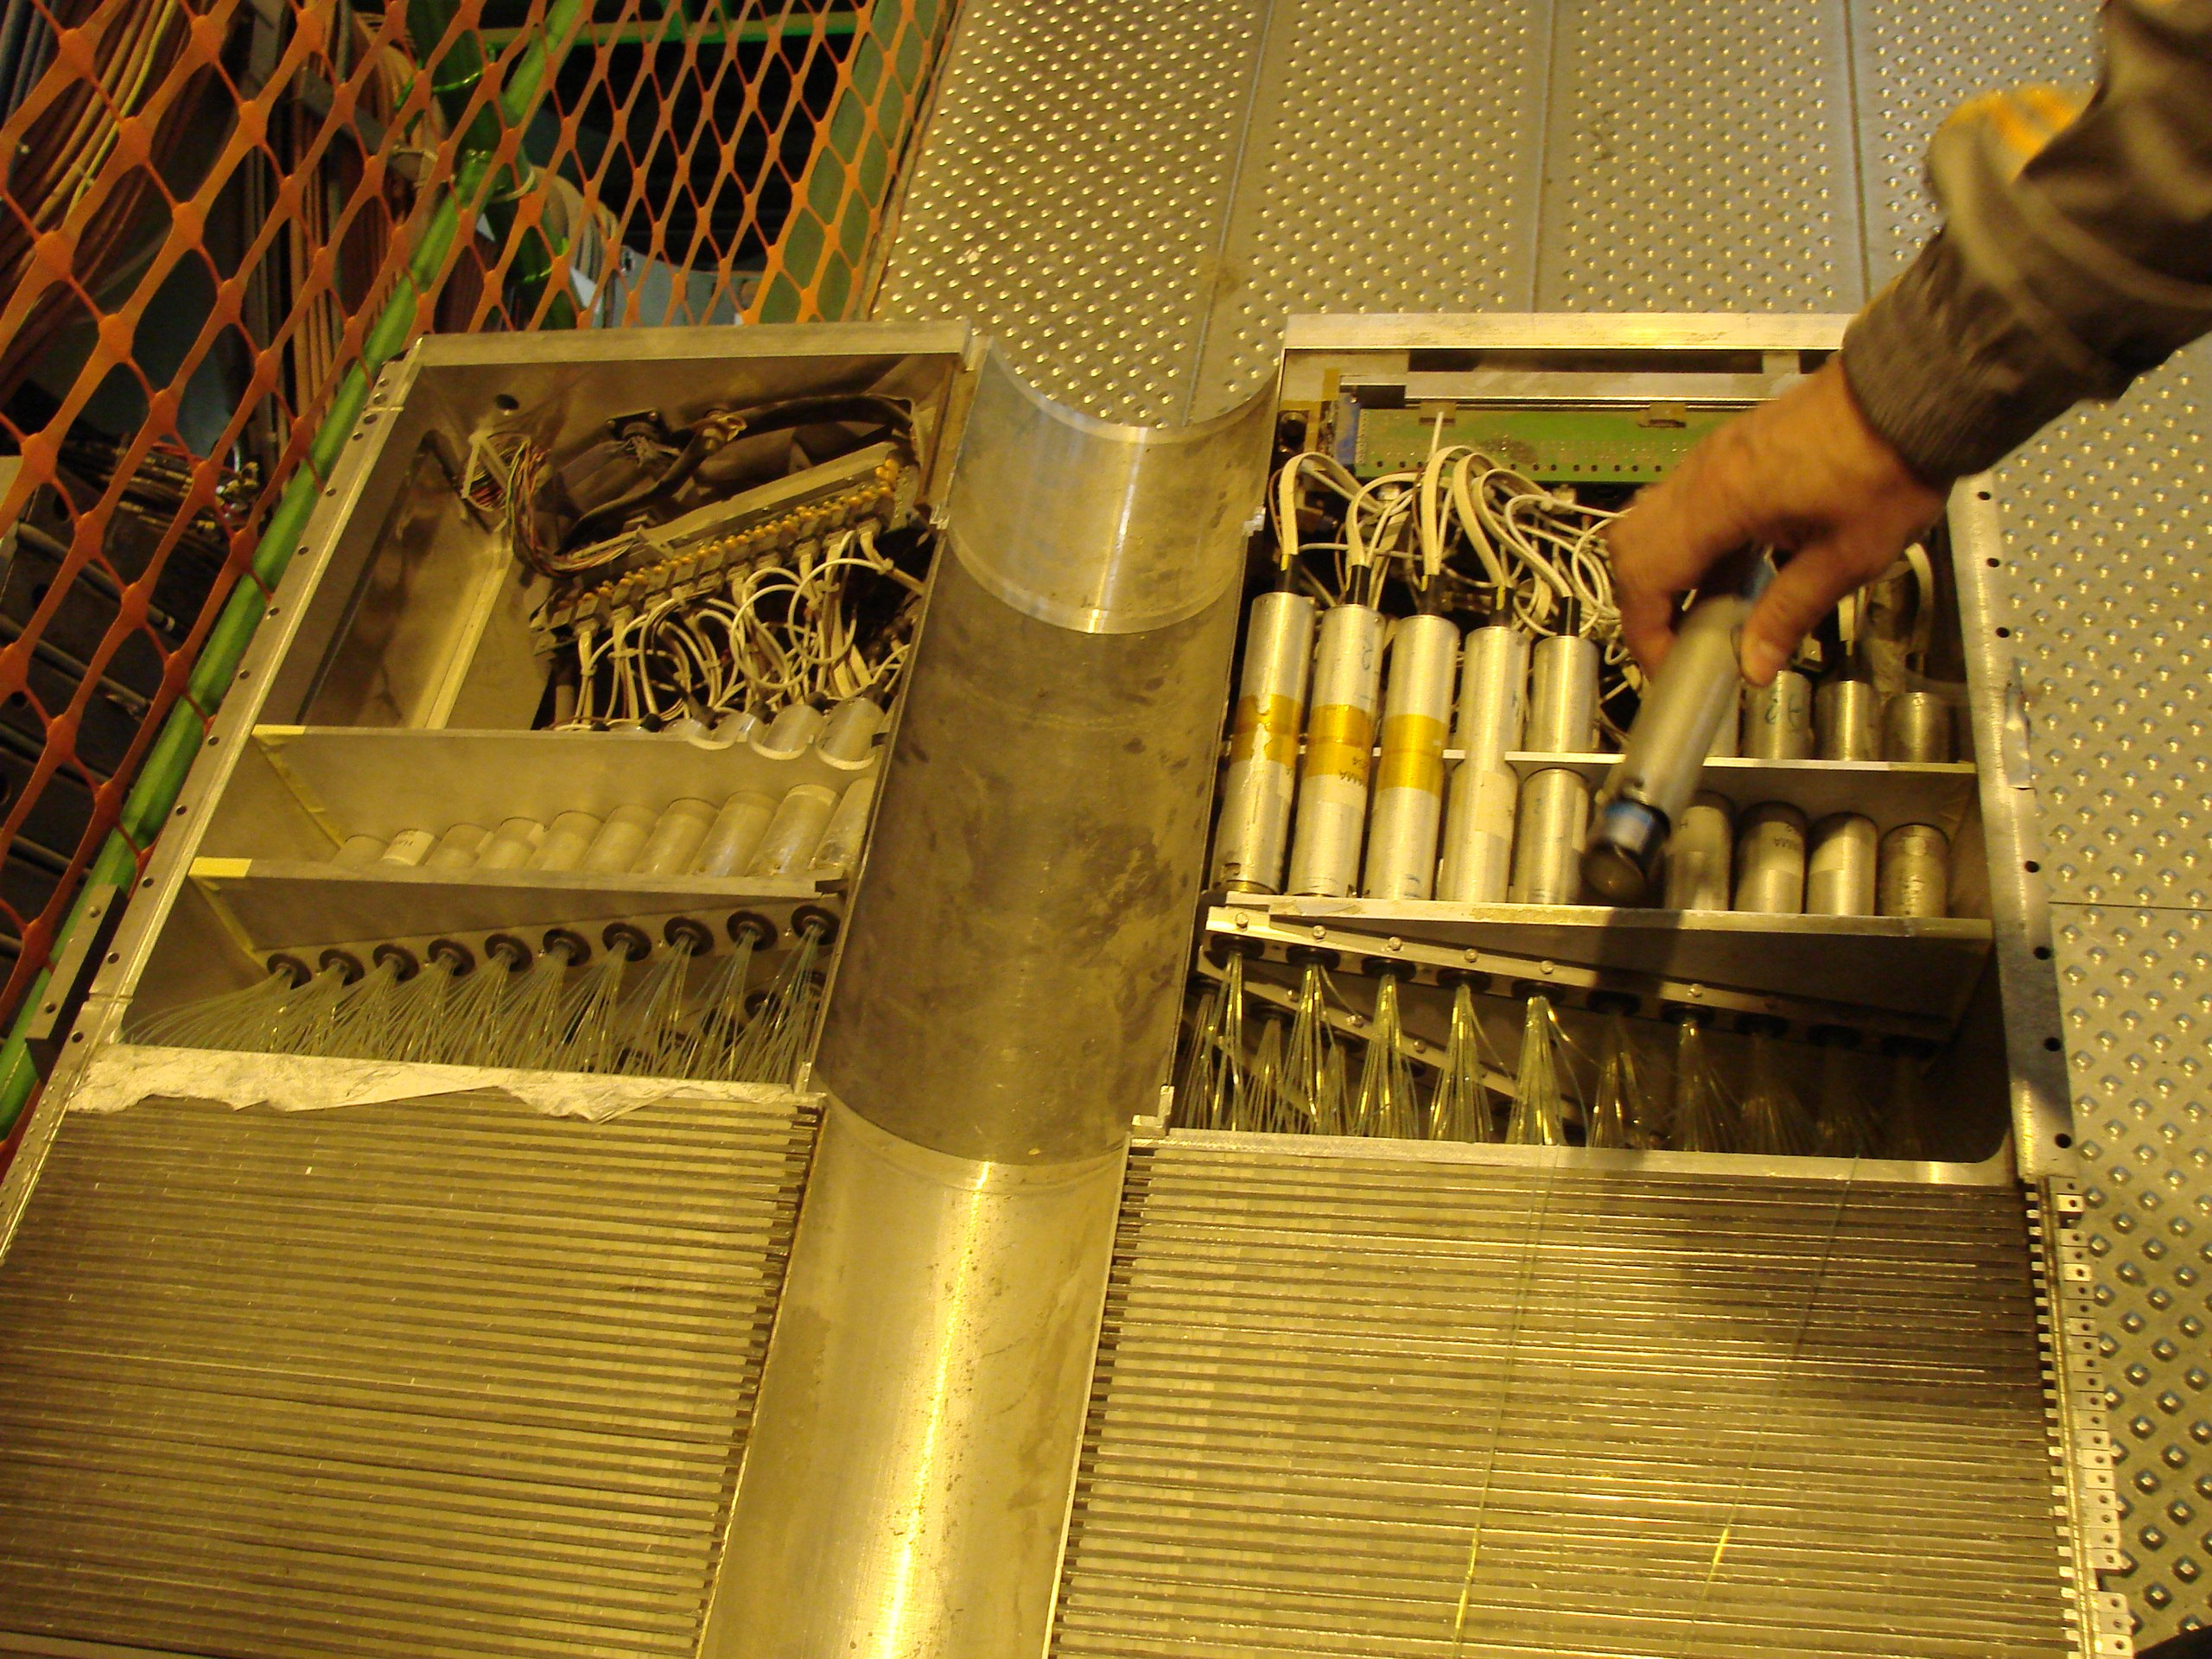
\includegraphics[width=0.7\textwidth]{hcal-pmt}
        \end{centering}
    \end{figure}
\end{frame}
\begin{frame}
    \begin{figure}
        \begin{centering}
            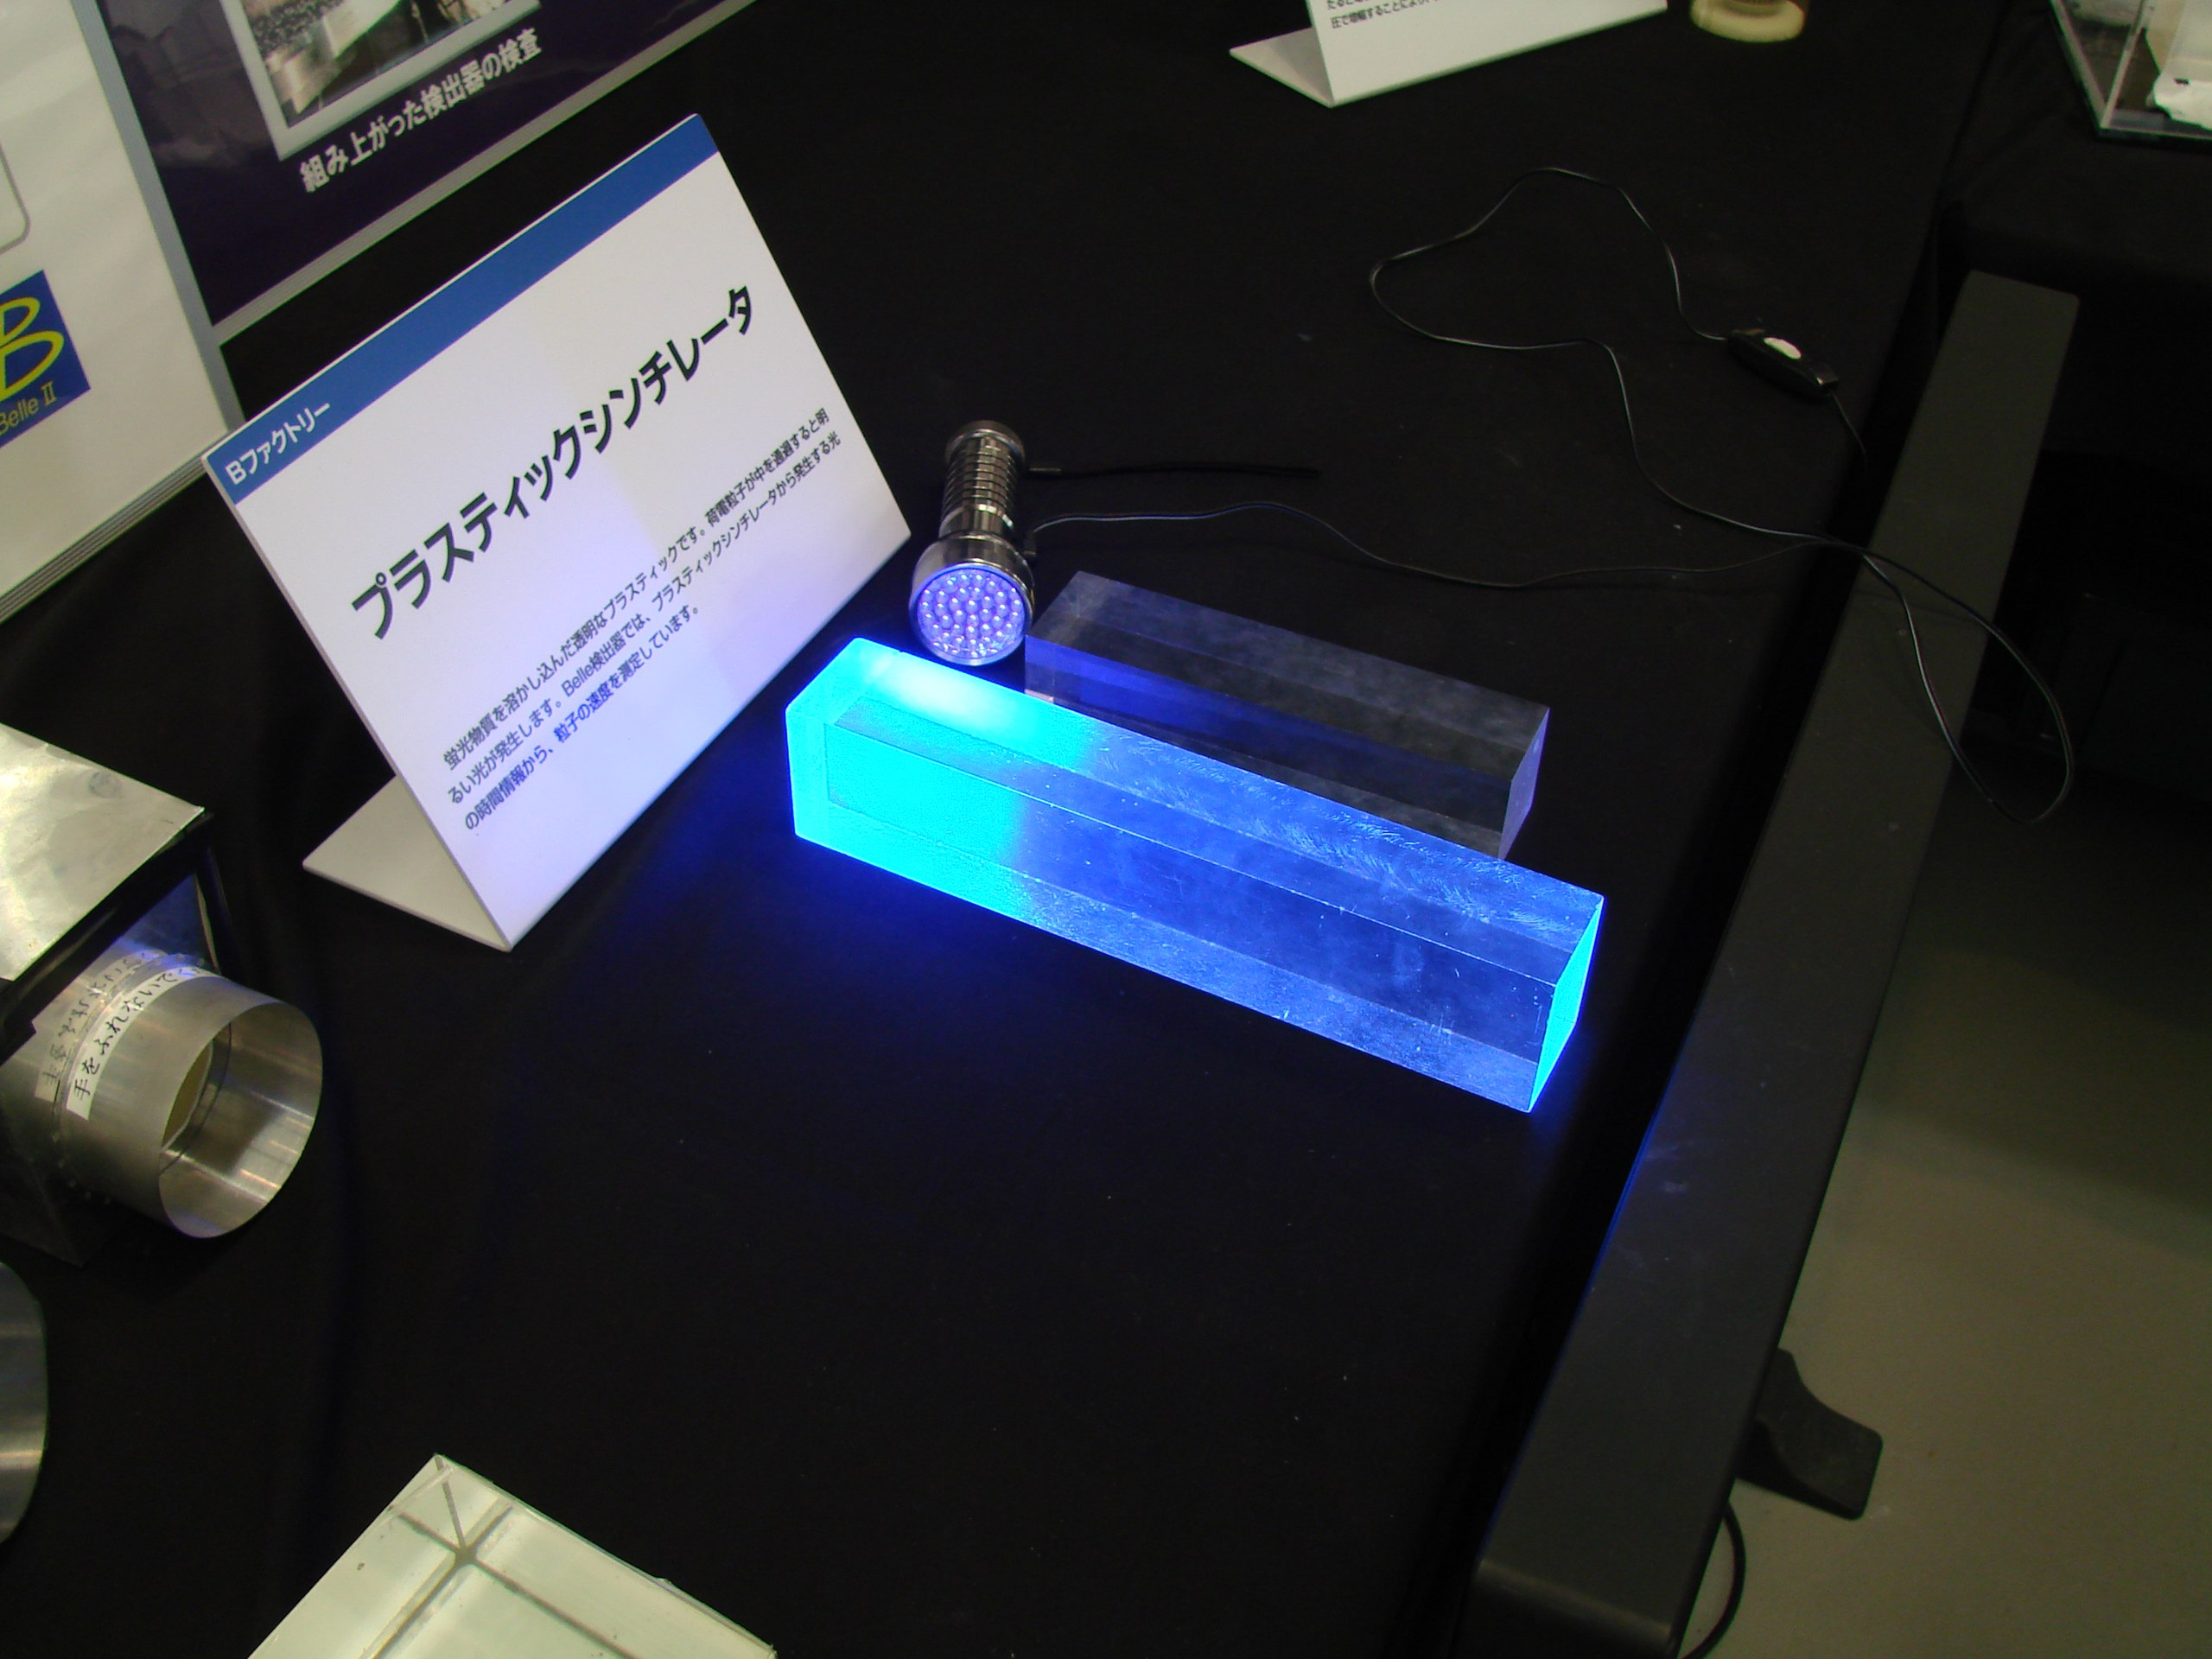
\includegraphics[width=0.7\textwidth]{scintillator}
        \end{centering}
    \end{figure}
\end{frame}

\begin{frame}
    \begin{figure}
    {\LARGE Эволюция ускорителей ЦЕРНа}
    \end{figure}
\end{frame}
\begin{frame}
    \frametitle{Ускорительный комплекс в ЦЕРНе}
    \begin{figure}
        \begin{centering}
            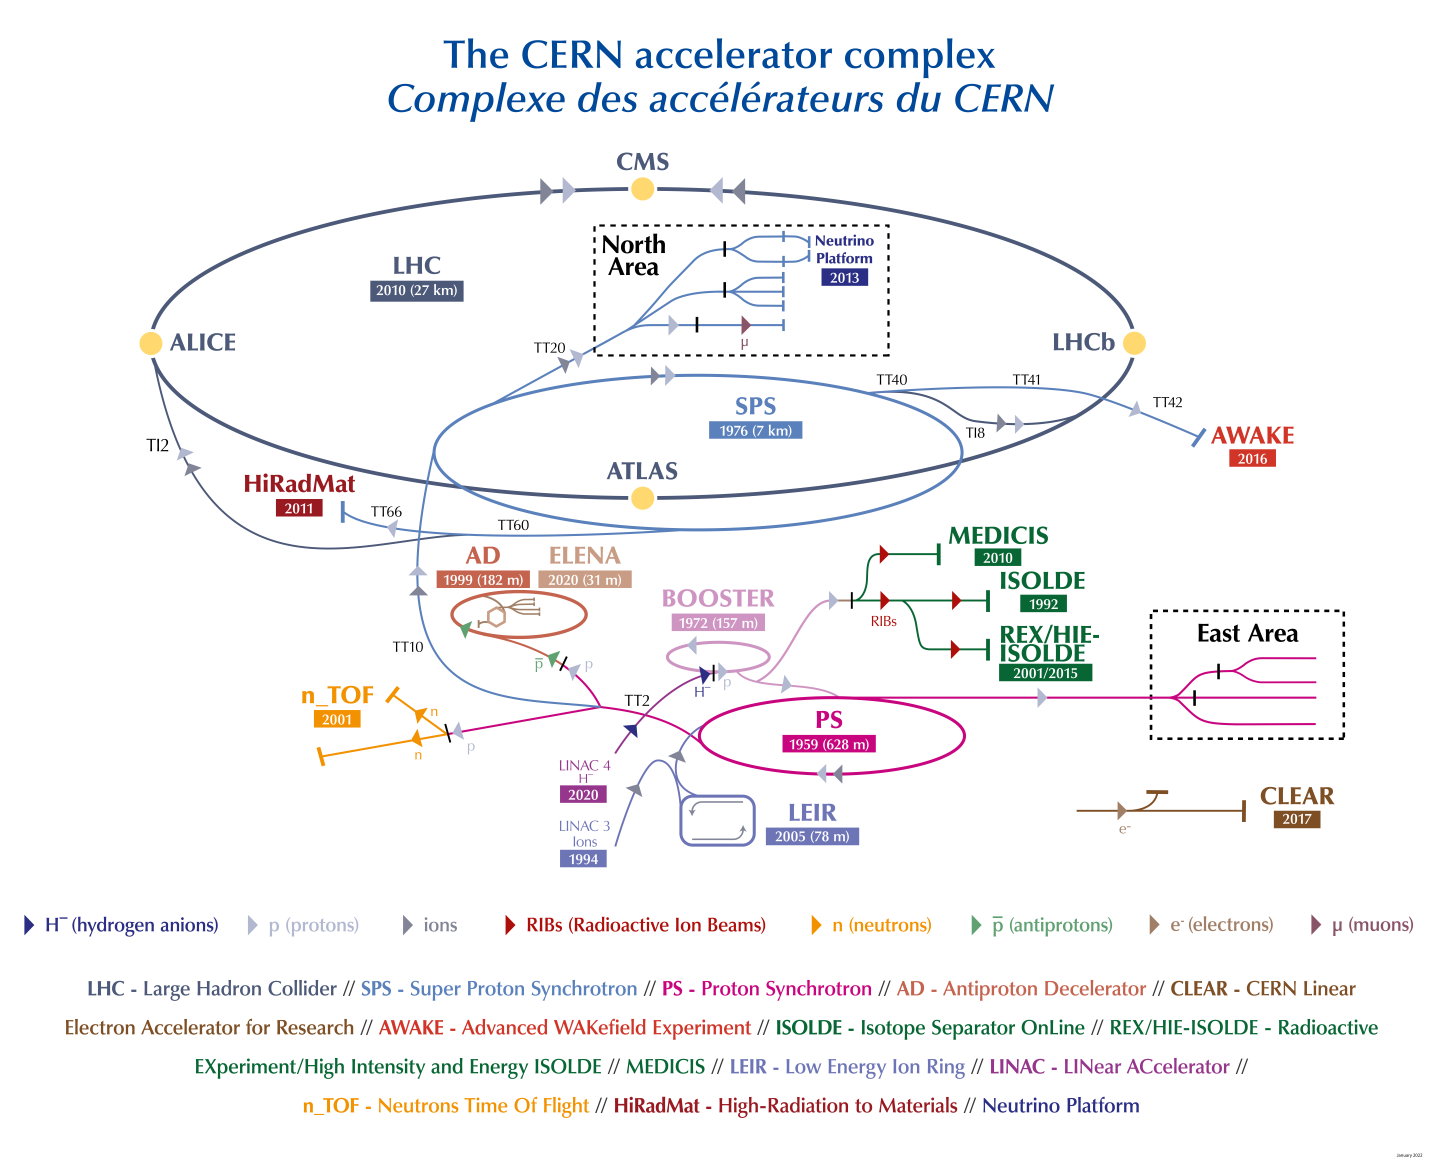
\includegraphics[width=0.7\textwidth]{accelerator-complex}
        \end{centering}
    \end{figure}
\end{frame}
\begin{frame}
    \frametitle{Протонный синхротрон}
    \begin{figure}
        \begin{centering}
            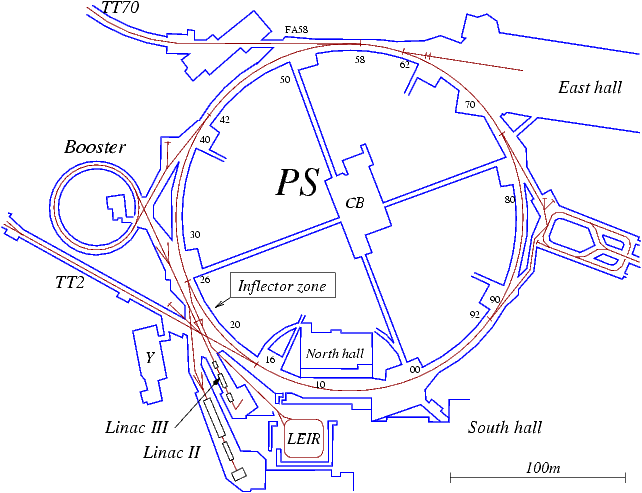
\includegraphics[width=0.7\textwidth]{ps}
        \end{centering}
    \end{figure}
\end{frame}
\begin{frame}
    \frametitle{Супер протон-антипротонный синхротрон}
    \begin{figure}
        \begin{centering}
            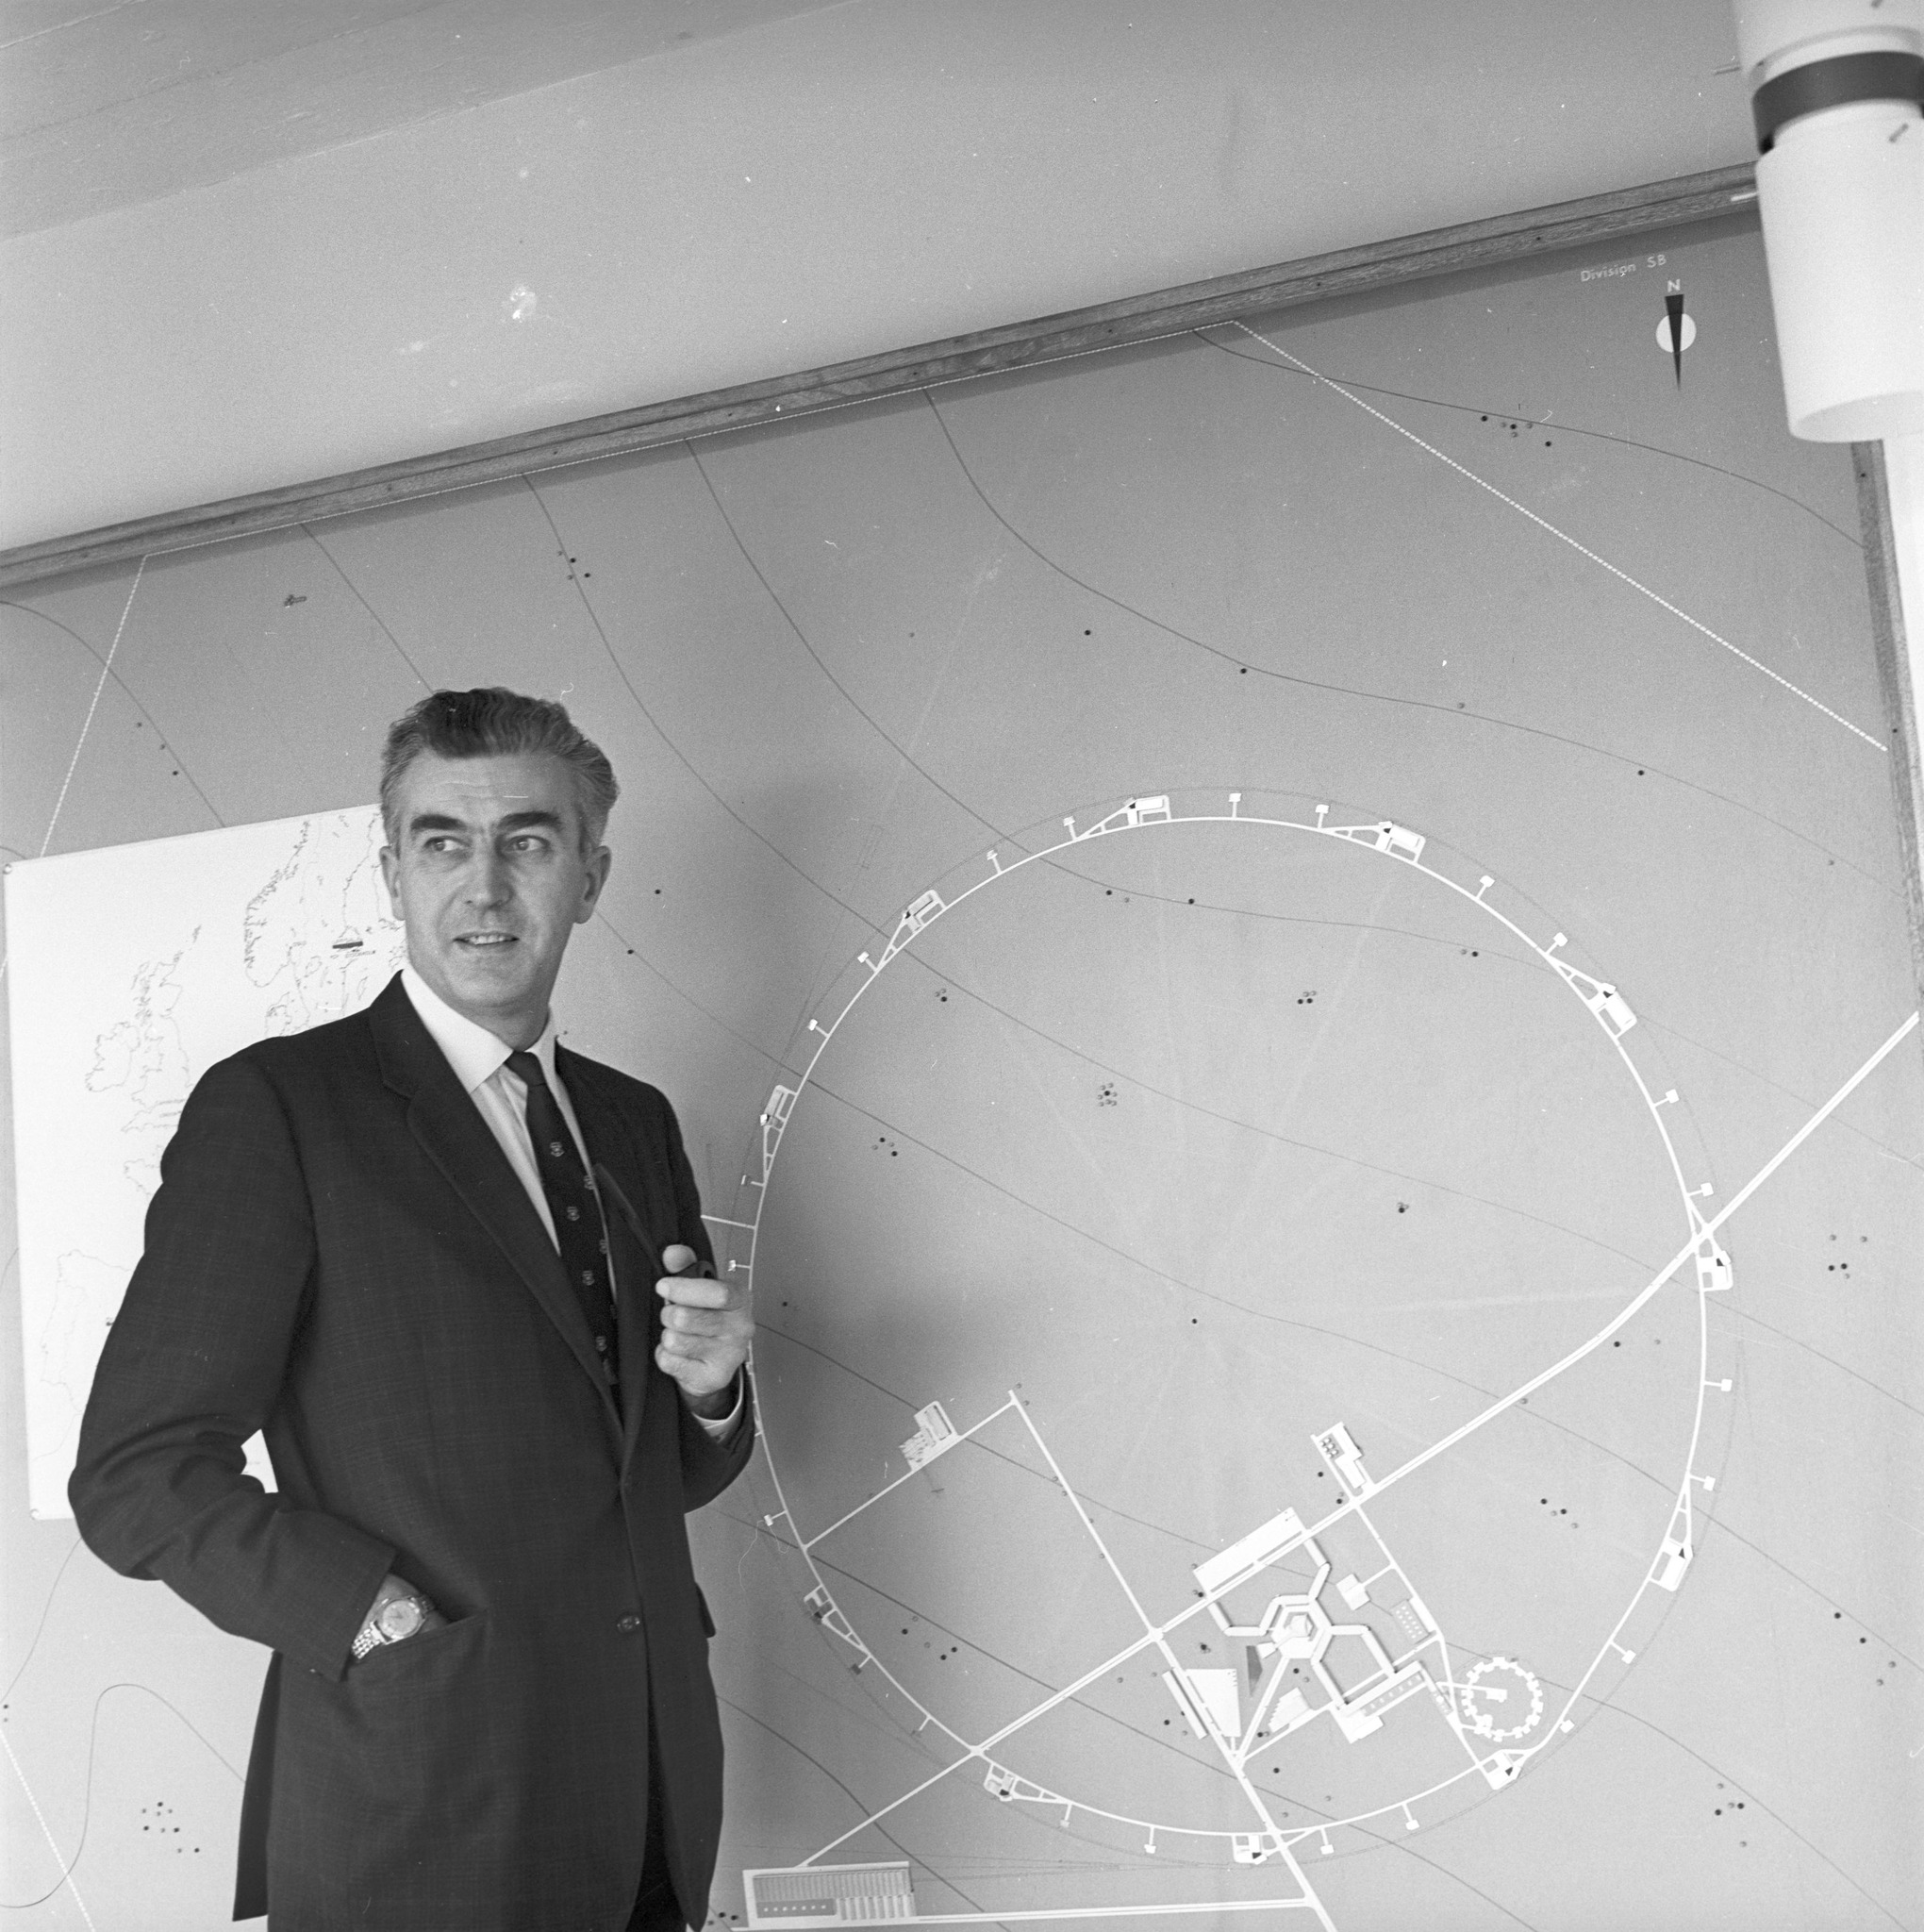
\includegraphics[width=0.5\textwidth]{spps}
        \end{centering}
    \end{figure}
\end{frame}
\begin{frame}
    \frametitle{Большой адронный коллайдер}
    \begin{figure}
        \begin{centering}
            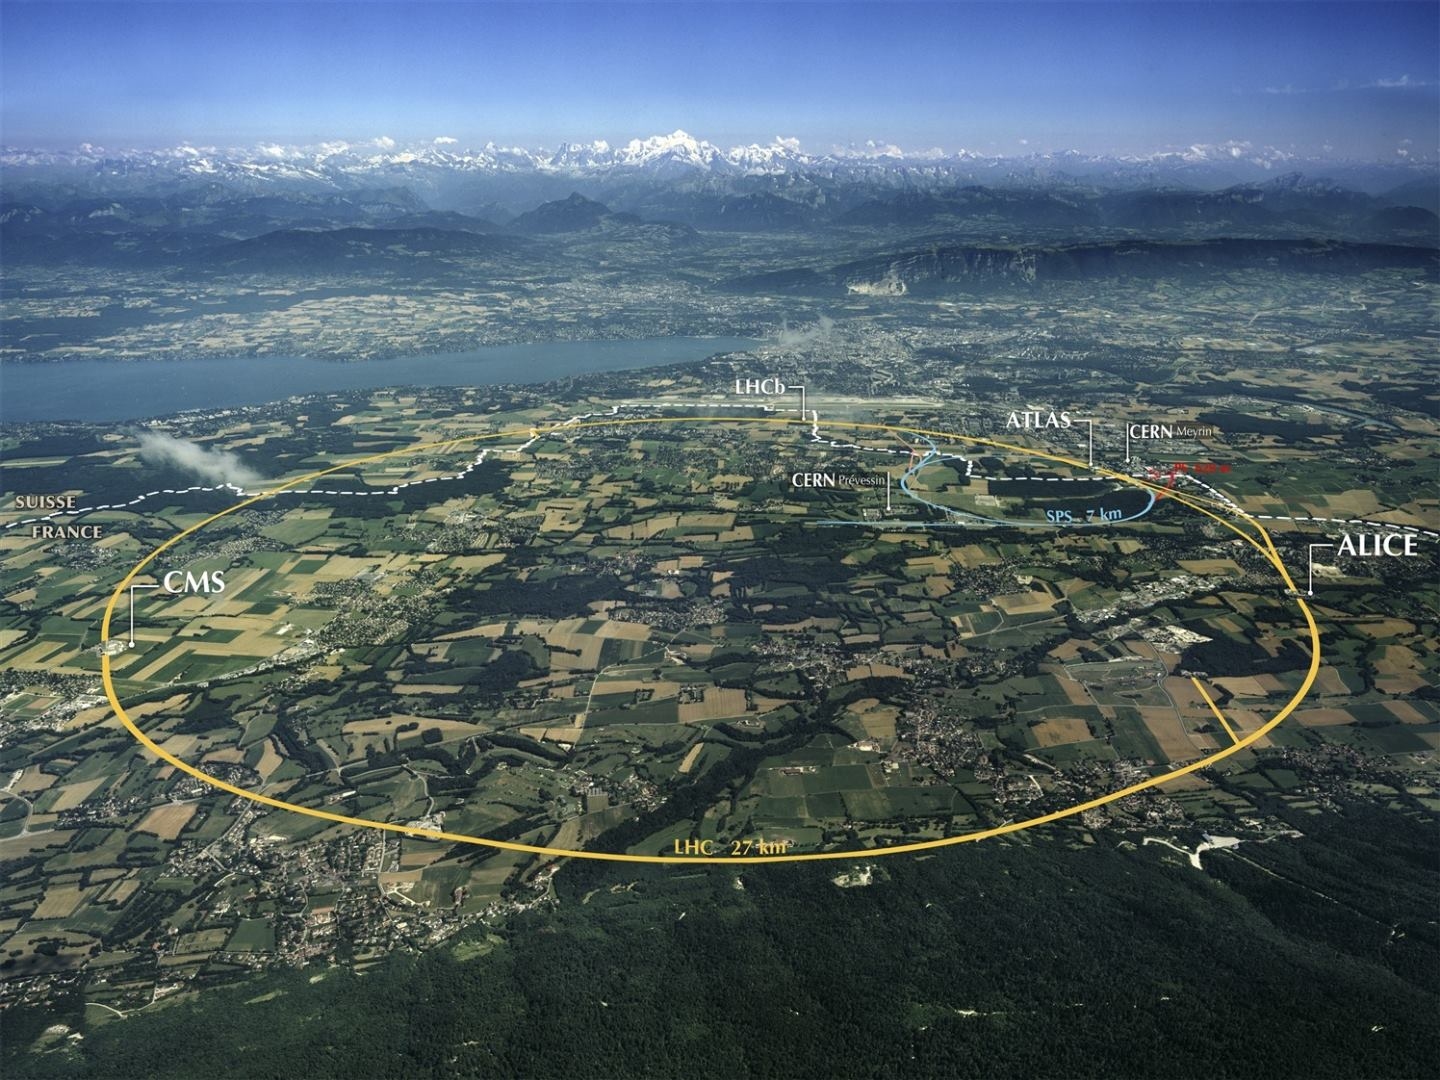
\includegraphics[width=0.7\textwidth]{lhc}
        \end{centering}
    \end{figure}
\end{frame}
\begin{frame}
    \frametitle{FCC: коллайдер XXI века}
    \begin{figure}
        \begin{centering}
            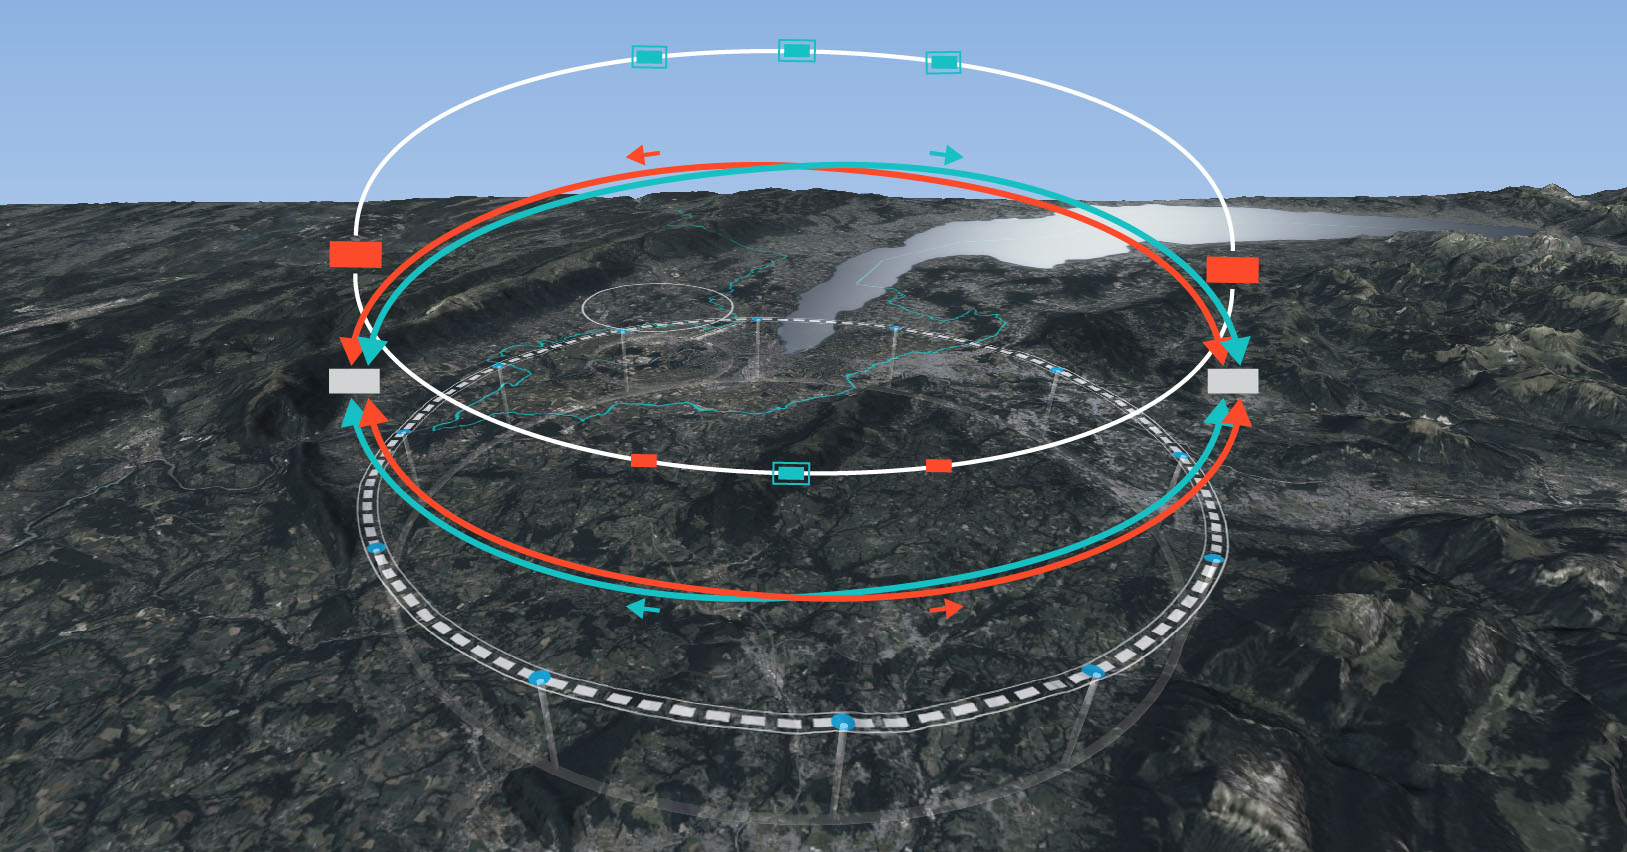
\includegraphics[width=0.7\textwidth]{fcc}
        \end{centering}
    \end{figure}
\end{frame}
